%%%%%%%%%%%%%%%%%%%%%%%%%%%%%%%%%%%%%%%%%%%%%%%%%%%%%%%%%%%%%%%
%% OXFORD THESIS TEMPLATE

% Use this template to produce a standard thesis that meets the Oxford University requirements for DPhil submission
%
% Originally by Keith A. Gillow (gillow@maths.ox.ac.uk), 1997
% Modified by Sam Evans (sam@samuelevansresearch.org), 2007
% Modified by John McManigle (john@oxfordechoes.com), 2015
%
% This version Copyright (c) 2015-2017 John McManigle
%
% Broad permissions are granted to use, modify, and distribute this software
% as specified in the MIT License included in this distribution's LICENSE file.
%

% I've (John) tried to comment this file extensively, so read through it to see how to use the various options.  Remember
% that in LaTeX, any line starting with a % is NOT executed.  Several places below, you have a choice of which line to use
% out of multiple options (eg draft vs final, for PDF vs for binding, etc.)  When you pick one, add a % to the beginning of
% the lines you don't want.


%%%%% CHOOSE PAGE LAYOUT
% The most common choices should be below.  You can also do other things, like replacing "a4paper" with "letterpaper", etc.

% This one will format for two-sided binding (ie left and right pages have mirror margins; blank pages inserted where needed):
\documentclass[a4paper,twoside]{ociamthesis}
% This one will format for one-sided binding (ie left margin > right margin; no extra blank pages):
%\documentclass[a4paper]{ociamthesis}
% This one will format for PDF output (ie equal margins, no extra blank pages):
%\documentclass[a4paper,nobind]{ociamthesis} 



%%%%% SELECT YOUR DRAFT OPTIONS
% Three options going on here; use in any combination.  But remember to turn the first two off before
% generating a PDF to send to the printer!

% This adds a "DRAFT" footer to every normal page.  (The first page of each chapter is not a "normal" page.)
\fancyfoot[C]{\emph{DRAFT Printed on \today}}  

% This highlights (in blue) corrections marked with (for words) \mccorrect{blah} or (for whole
% paragraphs) \begin{mccorrection} . . . \end{mccorrection}.  This can be useful for sending a PDF of
% your corrected thesis to your examiners for review.  Turn it off, and the blue disappears.
\correctionstrue


%%%%% BIBLIOGRAPHY SETUP
% Note that your bibliography will require some tweaking depending on your department, preferred format, etc.
% The options included below are just very basic "sciencey" and "humanitiesey" options to get started.
% If you've not used LaTeX before, I recommend reading a little about biblatex/biber and getting started with it.
% If you're already a LaTeX pro and are used to natbib or something, modify as necessary.
% Either way, you'll have to choose and configure an appropriate bibliography format...

% The science-type option: numerical in-text citation with references in order of appearance.
\usepackage[style=numeric-comp, sorting=none, backend=biber, doi=false, isbn=false]{biblatex}
\newcommand*{\bibtitle}{References}

% The humanities-type option: author-year in-text citation with an alphabetical works cited.
%\usepackage[style=authoryear, sorting=nyt, backend=biber, maxcitenames=2, useprefix, doi=false, isbn=false]{biblatex}
%\newcommand*{\bibtitle}{Works Cited}

% This makes the bibliography left-aligned (not 'justified') and slightly smaller font.
\renewcommand*{\bibfont}{\raggedright\small}

% Change this to the name of your .bib file (usually exported from a citation manager like Zotero or EndNote).
\addbibresource{references.bib}


% Uncomment this if you want equation numbers per section (2.3.12), instead of per chapter (2.18):
%\numberwithin{equation}{subsection}



%%%%% THESIS / TITLE PAGE INFORMATION
% Everybody needs to complete the following:
\title{Attosecond light: the laser-plasma surface interaction}
\author{Robin Timmis}
\college{Your College}

% Master's candidates who require the alternate title page (with candidate number and word count)
% must also un-comment and complete the following three lines:
%\masterssubmissiontrue
%\candidateno{933516}
%\wordcount{28,815}

% Uncomment the following line if your degree also includes exams (eg most masters):
%\renewcommand{\submittedtext}{Submitted in partial completion of the}
% Your full degree name.  (But remember that DPhils aren't "in" anything.  They're just DPhils.)
\degree{Doctor of Philosophy}
% Term and year of submission, or date if your board requires (eg most masters)
\degreedate{Michaelmas 2014}


%%%%% YOUR OWN PERSONAL MACROS
% This is a good place to dump your own LaTeX macros as they come up.
\usepackage[nolist]{acronym}
\usepackage{siunitx}


% To make text superscripts shortcuts
	\renewcommand{\th}{\textsuperscript{th}} % ex: I won 4\th place
	\newcommand{\nd}{\textsuperscript{nd}}
	\renewcommand{\st}{\textsuperscript{st}}
	\newcommand{\rd}{\textsuperscript{rd}}

%%%%% THE ACTUAL DOCUMENT STARTS HERE
\begin{document}



%%%%% CHOOSE YOUR LINE SPACING HERE
% This is the official option.  Use it for your submission copy and library copy:
\setlength{\textbaselineskip}{22pt plus2pt}
% This is closer spacing (about 1.5-spaced) that you might prefer for your personal copies:
%\setlength{\textbaselineskip}{18pt plus2pt minus1pt}

% You can set the spacing here for the roman-numbered pages (acknowledgements, table of contents, etc.)
\setlength{\frontmatterbaselineskip}{17pt plus1pt minus1pt}

% Leave this line alone; it gets things started for the real document.
\setlength{\baselineskip}{\textbaselineskip}


%%%%% CHOOSE YOUR SECTION NUMBERING DEPTH HERE
% You have two choices.  First, how far down are sections numbered?  (Below that, they're named but
% don't get numbers.)  Second, what level of section appears in the table of contents?  These don't have
% to match: you can have numbered sections that don't show up in the ToC, or unnumbered sections that
% do.  Throughout, 0 = chapter; 1 = section; 2 = subsection; 3 = subsubsection, 4 = paragraph...

% The level that gets a number:
\setcounter{secnumdepth}{2}
% The level that shows up in the ToC:
\setcounter{tocdepth}{2}


%%%%% ABSTRACT SEPARATE
% This is used to create the separate, one-page abstract that you are required to hand into the Exam
% Schools.  You can comment it out to generate a PDF for printing or whatnot.
\begin{abstractseparate}
	% Your abstract text goes here.  Check your departmental regulations, but generally this should be less than 300 words.  See the beginning of Chapter~\ref{ch:2-litreview} for more.

The commissioning of multi-petawatt class laser facilities around the world is gathering pace. One of the primary motivations for these investments is the acceleration of high-quality, low-emittance electron bunches. Here we explore the interaction of a high-intensity femtosecond laser pulse with a mass-limited dense target to produce MeV attosecond electron bunches in transmission and confirm with three-dimensional simulation that such bunches have low emittance and nano-Coulomb charge. We then perform a large parameter scan from non-relativistic laser intensities to the laser-QED regime and from the critical plasma density to beyond solid density to demonstrate that the electron bunch energies and the laser pulse energy absorption into the plasma can be quantitatively described via the Zero Vector Potential mechanism. These results have wide-ranging implications for future particle accelerator science and associated technologies.

Laser peak powers rise inexorably higher, enabling the study of increasingly exotic high energy density plasmas. This thesis explores one such phenomenon, that of the interaction between a relativistic laser pulse and a solid density plasma. The laser pulse is reflected but both the reflected radiation and the electron bunches that induce the interaction have fascinating properties

Electron bunches 


, including attosecond duration. Through the application of theory, simulation and experiment, this thesis strives to extend our understanding of this field and thus direct towards potential applications for these sources, primarily as a diagnostic tool. 

 % Create an abstract.tex file in the 'text' folder for your abstract.
\end{abstractseparate}


% JEM: Pages are roman numbered from here, though page numbers are invisible until ToC.  This is in
% keeping with most typesetting conventions.
\begin{romanpages}

% Title page is created here
\maketitle

%%%%% DEDICATION -- If you'd like one, un-comment the following.
%\begin{dedication}
%This thesis is dedicated to\\
%someone\\
%for some special reason\\
%\end{dedication}

%%%%% ACKNOWLEDGEMENTS -- Nothing to do here except comment out if you don't want it.
\begin{acknowledgements}
 	\subsection*{Personal}

\subsection*{Institutional}

The author thanks the Norreys Research Group, Prof. Philip Burrows and Dr. Qingsong Feng for useful discussions, the SMILEI consortium and the ARCHER2 support team. The authors also acknowledge the support of AWE plc, UKRI-EPSRC and the Oxford-Berman Graduate Scholarship program. This work used the ARCHER2 UK National Supercomputing Service (https://www.archer2.ac.uk) under project e674 of URKI-EPSRC grant no. EP/R029148/1 and UKRI-STFC grant no. ST/V001655/1.
\end{acknowledgements}

%%%%% ABSTRACT -- Nothing to do here except comment out if you don't want it.
\begin{abstract}
	% Your abstract text goes here.  Check your departmental regulations, but generally this should be less than 300 words.  See the beginning of Chapter~\ref{ch:2-litreview} for more.

The commissioning of multi-petawatt class laser facilities around the world is gathering pace. One of the primary motivations for these investments is the acceleration of high-quality, low-emittance electron bunches. Here we explore the interaction of a high-intensity femtosecond laser pulse with a mass-limited dense target to produce MeV attosecond electron bunches in transmission and confirm with three-dimensional simulation that such bunches have low emittance and nano-Coulomb charge. We then perform a large parameter scan from non-relativistic laser intensities to the laser-QED regime and from the critical plasma density to beyond solid density to demonstrate that the electron bunch energies and the laser pulse energy absorption into the plasma can be quantitatively described via the Zero Vector Potential mechanism. These results have wide-ranging implications for future particle accelerator science and associated technologies.

Laser peak powers rise inexorably higher, enabling the study of increasingly exotic high energy density plasmas. This thesis explores one such phenomenon, that of the interaction between a relativistic laser pulse and a solid density plasma. The laser pulse is reflected but both the reflected radiation and the electron bunches that induce the interaction have fascinating properties

Electron bunches 


, including attosecond duration. Through the application of theory, simulation and experiment, this thesis strives to extend our understanding of this field and thus direct towards potential applications for these sources, primarily as a diagnostic tool. 


\end{abstract}

%%%%% MINI TABLES
% This lays the groundwork for per-chapter, mini tables of contents.  Comment the following line
% (and remove \minitoc from the chapter files) if you don't want this.  Un-comment either of the
% next two lines if you want a per-chapter list of figures or tables.
\dominitoc % include a mini table of contents
%\dominilof  % include a mini list of figures
%\dominilot  % include a mini list of tables

% This aligns the bottom of the text of each page.  It generally makes things look better.
\flushbottom

% This is where the whole-document ToC appears:
\tableofcontents

\listoffigures
	\mtcaddchapter
% \mtcaddchapter is needed when adding a non-chapter (but chapter-like) entity to avoid confusing minitoc

% Uncomment to generate a list of tables:
%\listoftables
%	\mtcaddchapter

%%%%% LIST OF ABBREVIATIONS
% This example includes a list of abbreviations.  Look at text/abbreviations.tex to see how that file is
% formatted.  The template can handle any kind of list though, so this might be a good place for a
% glossary, etc.
% First parameter can be changed eg to "Glossary" or something.
% Second parameter is the max length of bold terms.
\begin{mclistof}{A List of Symbols and Abbreviations}{3.2cm}

\item[$e$] Absolute charge of an electron = \qty{1.602e-19}{C}
\item[$\epsilon_0$] Permittivity of free space = \qty{8.854e-12}{F.m^{-1}}
\item[$\lambda_D$]Debye length $\equiv \sqrt{\frac{\epsilon_0KT_e}{n_ee^2}}$
\item[$n_e$] Plasma electron number density as a function of position
\item[$n_i$] Plasma ion number density as a function of position
\item[$T_e$] Plasma electron temperature
\item[$Z$] Ion charge state in units of $e$

\item[1D, 2D, 3D] One-, two- or three-dimension(al)

\item[Otter] One of the finest of water mammals.

\item[Hedgehog] Quite a nice prickly friend.

\begin{acronym}
	\acro{1D}{one-dimension}
	\acro{2D}{two-dimensions}
	\acro{3D}{three-dimensions}
	\acro{FDTD}{Finite Difference Time Domain}
	\acro{HHG}{High Harmonic Generation}
	\acro{QED}{Quantum Electro-Dynamics}
	\acro{PIC}{Particle-In-Cell}
	\acro{ZVP}{Zero Vector Potential}
\end{acronym}

\end{mclistof} 


% The Roman pages, like the Roman Empire, must come to its inevitable close.
\end{romanpages}


%%%%% CHAPTERS
% Add or remove any chapters you'd like here, by file name (excluding '.tex'):
\flushbottom
\chapter{\label{ch:1-intro}Introduction} 

\minitoc

% TODO 
%{A plan}


%sections to include
% Start with the laser and our entrance into the multi-petawatt regime with no signs of stopping - ref 40 in Alex Savin's thesis - it looks like that is saying huge growth in laser power check that and maybe write in the thesis but don't include the figure. Also, include a description of CPA and OPCPA
%intense lasers and absorption mechanisms?? yes for sure but don't do all those just below ZVP
%Frames of reference - lab, sim, ablating front surface of plasma

% What is the story? Based on the first section by Alex after the abstract
%Plasma is ubiquitous in our known universe and plasma provides us with huge opportunities as a tool to improve our lives
%Simulataneously our ability to understand physics has been aided by an explosion in computing power (Peter HEDP paper)
%In this thesis we discuss some of the opportunities that relativistic laser plasma physics offers us with solid density targets - note that note about solids v gases at this point. 
%Perhaps even before the debye length, define what we mean by the temperature of the plasma.

%An unused statement about ion immobility
%Assume for now that the ion-electron mass ratio is infinite, that is to say, the ions are approximately immobile for the timescales under consideration, generally true for a fair few relativistic laser pulse cycles (In later sections the mobility of plasma ions will prove very important but for now this is ignored.).
% I should also discuss ionisation and laser surface plasma interaction./

\section{High-energy-density physics}
We sit on the verge of the exascale revolution, in both computing resources \cite{kotheExascaleComputingUnited2019} and laser power. With rapid adoption of the pioneering advancements of Chirped Pulse Amplification (CPA) by Strickland and Mourou \cite{stricklandCompressionAmplifiedChirped1985} and of Optical Parametric Chirped Pulse Amplification \cite{rossOpticalParametricChirped2000}, multi-petawatt facilities have been commissioned and built across the globe and plans for sub-exawatt facilities are now underway. Figure \ref{fig:intro_lasersystems} details the parameter space accessible by current and proposed facilities \cite{stricklandCompressionAmplifiedChirped1985, fourmauxPedestalCleaningHigh2011, wang085PWLaser2017, tiscarenoOhioStateUniversity2020, sung42PW202017, rossGenerationTerawattPulses2000, yangMultiterawattLaserSystem2002, witte2006source, stoecklHighEnergyPetawattProject2006, lozhkarevCompact56Petawatt2007, herrmannGenerationSubthreecycle162009, andriukaitis90GWPeak2011, zhaoGeneration120GW2013, hoppsOverviewLaserSystems2013, hoppsOverviewLaserSystems2013, thire10MJ5cycle2015, yinHighefficiencyOpticalParametric2016, galesExtremeLightInfrastructure2018, OMEGAFacility, renCompactDoublepassRaman2008, lanciaExperimentalEvidenceShort2010, lanciaSignaturesSelfSimilarRegime2016, marquesJouleLevelHighEfficiencyEnergy2019, thebergeTunableUltrashortLaser2006, trushinSub10fsSupercontinuumRadiation2007, ohIntenseTerahertzGeneration2013, horioGenerationSub17Fs2014, takahashiGeneration10uJCoherent2002, goulielmakisSingleCycleNonlinearOptics2008, skantzakisCoherentContinuumExtreme2009, ferrariHighenergyIsolatedAttosecond2010, takahashiAttosecondNonlinearOptics2013, popmintchevUltravioletSurpriseEfficient2015, nomuraAttosecondPhaseLocking2009, bierbachGeneration10Relativistic2012, heisslerMultimJHarmonicEmission2015, yeungExperimentalObservationAttosecond2017, jahnIntenseIsolatedAttosecond2019, rusEfficientHighbrightnessSoftxray1997, sebbanFullCharacterizationHighgain2000, rusMultimillijouleHighlyCoherent2002, zeitounHighintensityHighlyCoherent2004, wangHighBrightnessInjectionSeededSoftXRayLaser2006, rohringerAtomicInnershellXray2012, ayvazyanFirstOperationFreeelectron2006, ackermannOperationFreeelectronLaser2007, emmaFirstLasingOperation2010, FlashFreeElectronLaser, FlashFreeElectronLaser, FELIXLaboratoryOverview, FELIXLaboratoryOverview, FELIXLaboratoryOverview, kneipObservationSynchrotronRadiation2008, kneipBrightSpatiallyCoherent2010, juEnhancementXraysGenerated2012, chenBrightBetatronXray2013, wangQuasimonoenergeticLaserplasmaAcceleration2013, coleLaserwakefieldAcceleratorsHard2015, wenzQuantitativeXrayPhasecontrast2015, taphuocAllopticalComptonGammaray2012, chenMeVEnergyRaysInverse2013, tsaiCompactTunableCompton2015, polyanskiyPicosecondPulseAmplification2011, haberbergerFifteenTerawattPicosecond2010, glowniaAmplification193nmFemtosecond1992, kandoEnhancementPhotonNumber2009, obenschainHighenergyKryptonFluoride2015, trinesSimulationsEfficientRaman2011, trinesSimulationsEfficientRaman2011, kawanakaConceptualDesignSubexawatt2016, tajimaMarriage20keVSuperconducting2018}, clearly, there is no indication of wavering interest or support for the field of \ac{HED} physics. 
\begin{figure}
	\centering
	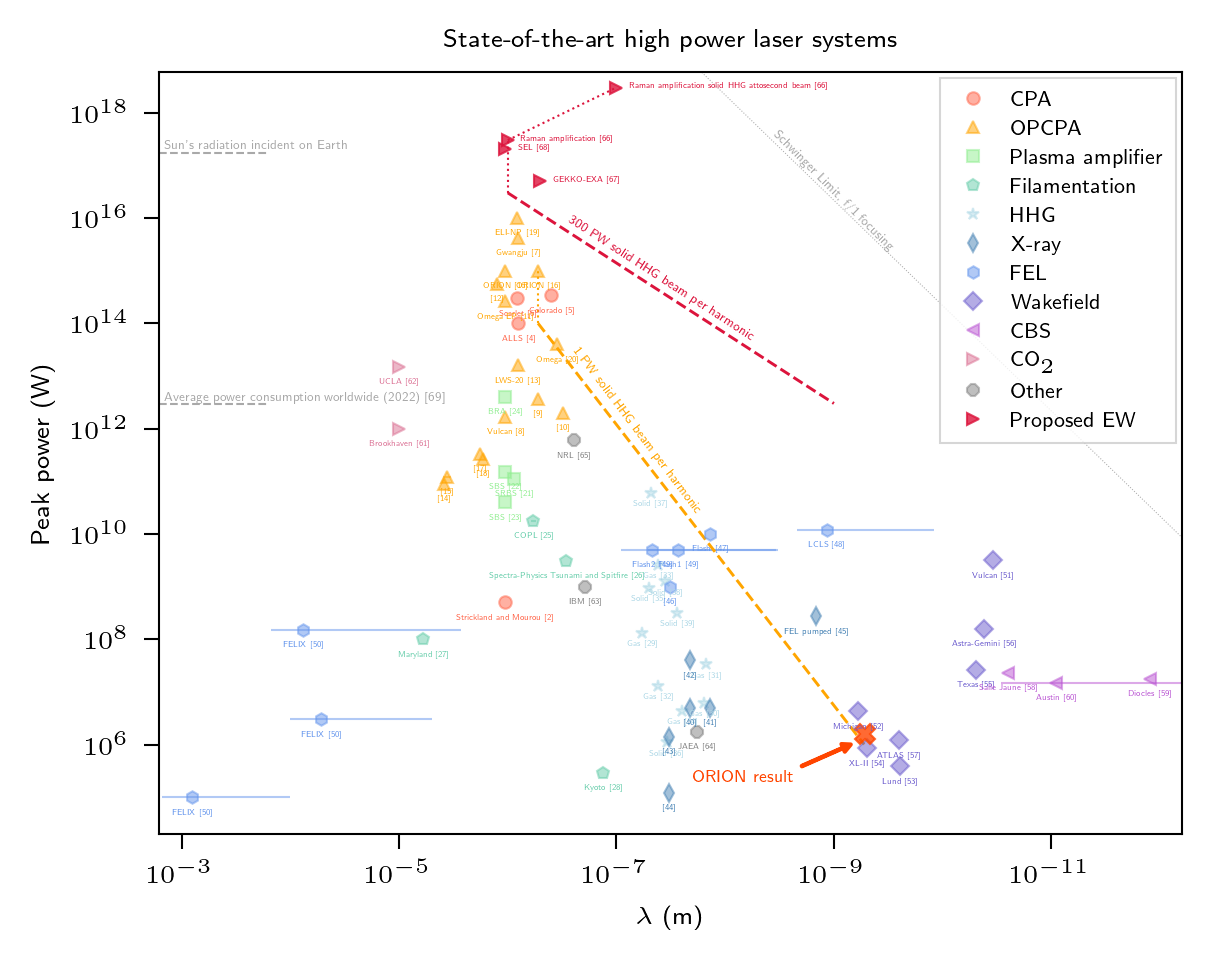
\includegraphics[width=\linewidth]{figures/intro/laser_systems}
	\caption[Laser systems across the globe, both commissioned, planned and theorised. theorised.]{A by no means exhaustive plot of high power light producing facilities from across the globe, both commissioned, planned and theorised \cite{stricklandCompressionAmplifiedChirped1985, fourmauxPedestalCleaningHigh2011, wang085PWLaser2017, tiscarenoOhioStateUniversity2020, sung42PW202017, rossGenerationTerawattPulses2000, yangMultiterawattLaserSystem2002, witte2006source, stoecklHighEnergyPetawattProject2006, lozhkarevCompact56Petawatt2007, herrmannGenerationSubthreecycle162009, andriukaitis90GWPeak2011, zhaoGeneration120GW2013, hoppsOverviewLaserSystems2013, hoppsOverviewLaserSystems2013, thire10MJ5cycle2015, yinHighefficiencyOpticalParametric2016, galesExtremeLightInfrastructure2018, OMEGAFacility, renCompactDoublepassRaman2008, lanciaExperimentalEvidenceShort2010, lanciaSignaturesSelfSimilarRegime2016, marquesJouleLevelHighEfficiencyEnergy2019, thebergeTunableUltrashortLaser2006, trushinSub10fsSupercontinuumRadiation2007, ohIntenseTerahertzGeneration2013, horioGenerationSub17Fs2014, takahashiGeneration10uJCoherent2002, goulielmakisSingleCycleNonlinearOptics2008, skantzakisCoherentContinuumExtreme2009, ferrariHighenergyIsolatedAttosecond2010, takahashiAttosecondNonlinearOptics2013, popmintchevUltravioletSurpriseEfficient2015, nomuraAttosecondPhaseLocking2009, bierbachGeneration10Relativistic2012, heisslerMultimJHarmonicEmission2015, yeungExperimentalObservationAttosecond2017, jahnIntenseIsolatedAttosecond2019, rusEfficientHighbrightnessSoftxray1997, sebbanFullCharacterizationHighgain2000, rusMultimillijouleHighlyCoherent2002, zeitounHighintensityHighlyCoherent2004, wangHighBrightnessInjectionSeededSoftXRayLaser2006, rohringerAtomicInnershellXray2012, ayvazyanFirstOperationFreeelectron2006, ackermannOperationFreeelectronLaser2007, emmaFirstLasingOperation2010, FlashFreeElectronLaser, FlashFreeElectronLaser, FELIXLaboratoryOverview, FELIXLaboratoryOverview, FELIXLaboratoryOverview, kneipObservationSynchrotronRadiation2008, kneipBrightSpatiallyCoherent2010, juEnhancementXraysGenerated2012, chenBrightBetatronXray2013, wangQuasimonoenergeticLaserplasmaAcceleration2013, coleLaserwakefieldAcceleratorsHard2015, wenzQuantitativeXrayPhasecontrast2015, taphuocAllopticalComptonGammaray2012, chenMeVEnergyRaysInverse2013, tsaiCompactTunableCompton2015, polyanskiyPicosecondPulseAmplification2011, haberbergerFifteenTerawattPicosecond2010, glowniaAmplification193nmFemtosecond1992, kandoEnhancementPhotonNumber2009, obenschainHighenergyKryptonFluoride2015, trinesSimulationsEfficientRaman2011, trinesSimulationsEfficientRaman2011, kawanakaConceptualDesignSubexawatt2016, tajimaMarriage20keVSuperconducting2018, NetElectricityConsumption, umstadterRelativisticLaserPlasma2003, dollarEnhancedLaserAbsorption2017} to provide an overview of the parameter space currently and soon to be accessible. The experimental result obtained at the ORION laser facility \cite{hoppsOverviewLaserSystems2013} is included, and will be discussed in detail in chapter \ref{ch:3-orion}. The dashed orange line is from the relevant theoretical model. The red dashed line marks the parameter space attainable via the methods discussed in this thesis when coupled with a sub-etawatt laser pulse. Such a beamline would provide intensities in the water window many orders of magnitude beyond that currently available from state-of-the-art facilities. }
	\label{fig:intro_lasersystems}
\end{figure}

\ac{HED} physics is the laboratory study of the behaviour of matter with a pressure above \qty{10}{GPa}, approximately one million atmospheres, and containing free electrons not confined to a solid state \cite{drakeFocusHighEnergy2014}, typically in the plasma state of matter. \ac{HED} conditions are found for a vast range of densities and temperatures (from zero to a million million Kelvin) and operating in both the quantum and relativistic realms. The applications are equally diverse, including but not limited to inertial confinement fusion, particle acceleration for scientific or medical purposes and light sources as diagnostic tools. Ubiquitous in the natural universe, beyond our solar system, all that can be observed in the sky is radiation emitted from \ac{HED} plasmas \cite{chenIntroductionPlasmaPhysics2016}.

Independently, the field of attosecond physics has flourished \cite{krauszAttosecondPhysics2009}. By irradiating gas targets with mildly ionising laser pulse intensities, pulses of attosecond radiation, composed of high-order harmonics of the laser, have been generated. Recognised by the 2023 Nobel Prize for Physics, the research of Agostini, Krausz and Huillier has revealed the inner workings of atoms and molecules, tracking fundamental electronic dynamics \cite{ElectronilluminatingLaserPulses2023}. At the intersection of HED and attosecond physics, there is another course for the generation of harmonics with the potential to produce brighter and shorter pulses than those of the laser-gas interaction. This thesis concerns itself with that interaction, that of a high-power short-pulse laser incident on a flat solid target. Through the processes here discussed, state-of-the-art 10 PW laser facilities such as ELI-np \cite{galesExtremeLightInfrastructure2018} can produce electron bunches and light pulses of exceptional charge and brightness, and of attosecond duration, thus uncovering new avenues for attosecond resolution diagnostics and for probing vacuum non-linearities. 

Seemingly counter-intuitively, as the laser power increases, via relativistic effects and for particular initial conditions, greater coherency in electron dynamics can be observed and signals are amplified. Before delving into this fascinating phenomenon, the remainder of this chapter provides some of the relevant background information. Chapter \ref{ch:2-zvp} introduces the \ac{ZVP} model of attosecond absorption to describe this laser-solid interaction. Chapter \ref{ch:3-orion} focuses instead on the reflected radiation and its high harmonic content, specifically with regard to the measurement of X-ray harmonics on the March 2023 ORION experiment. This chapter accessed a moderately different regime to that of \ac{ZVP}. Chapter \ref{ch:4-gemini} brings together both absorption and reflection in the ZVP regime, detailing the upcoming GEMINI PW experiment. Finally, Chapter \ref{ch:5-summary} summarises the body of work covered by this thesis and discusses potential future work.

% TODO add an extra line on computing power

\section{Electromagnetism fundamentals}
The spatiotemporal propagation of electric $\mathbf{E}(t,\mathbf{x})$ and magnetic $\mathbf{B}(t,\mathbf{x})$ fields must satisfy Maxwell's equations \cite{chenIntroductionPlasmaPhysics2016}
\begin{subequations}
	\label{eq:intro-maxwell}
	\begin{align}
		\nabla \cdot \mathbf{B} &= 0, \label{eq:intro-B0} \\
		\nabla \cdot \mathbf{E} &= \frac{\rho}{\epsilon_0},\label{eq:intro-E0} \\
		\nabla \times \mathbf{B} &= \mu_0 \mathbf{J} + \mu_0 \epsilon_0 \partial_t \mathbf{E},\label{eq:intro-B1} \\
		\nabla \times \mathbf{E} &=-\partial_t \mathbf{B}. \label{eq:intro-E1}
	\end{align}
\end{subequations}
Here, $\epsilon_0 = \qty{8.85e-12}{F.m^{-1}}$ and $\mu_0 = \qty{1.26e-6}{N.A^{-2}}$ are the vacuum permittivity and permeability respectively and $\rho(t,\mathbf{x})$ and $\mathbf{J}(t,\mathbf{x})$ the total charge and current densities of the charged particles present in the system. 

A particle with charge $q$ and velocity $\mathbf{v}$ in the presence of electromagnetic fields experiences the Lorentz force,
\begin{equation}\label{eq:intro-Lorentz_force}
	\mathbf{F}_\mathrm{L} = q(\mathbf{E} + \mathbf{v} \times \mathbf{B}).
\end{equation}

The electromagnetic fields can be obtained from the scalar, $\phi$, and vector, $\mathbf{A}$, potentials as  \cite{steaneRelativityMadeRelatively2012}
\begin{equation}
	\mathbf{E} = -\nabla \phi - \partial_t \mathbf{A},
\end{equation}
\begin{equation}
	\mathbf{B} = \nabla \times \mathbf{A}.
\end{equation}

\subsubsection{The Vlasov-Maxwell system of equations}
A collisionless and fully ionised plasma is fully described in the kinetic description by the Vlasov-Maxwell system of equations \cite{derouillatSmileiCollaborativeOpensource2018}. Each plasma species, $s$, of particles with mass $m_s$ and charge $q_s$ is represented by its distribution function $f_s(t,\mathbf{x},\mathbf{p})$ at time $t$, position $\mathbf{x}$ and momentum $\mathbf{p} = m_s \gamma \mathbf{v}$. The distribution satisfies the Vlasov equation, that is,
\begin{equation}\label{eq:intro-vlasov}
	(\partial_t + \frac{\mathbf{p}}{m_s\gamma} \cdot \nabla + \mathbf{F}_\mathrm{L} \cdot \nabla_\mathbf{p})f_s = 0,
\end{equation}
where $\mathbf{F}_\mathrm{L}$ is the Lorentz force given in equation \ref{eq:intro-Lorentz_force}. The electric $\mathbf{E}(t,\mathbf{x})$ and magnetic $\mathbf{B}(t,\mathbf{x})$ fields that generate the force must satisfy Maxwell's Equations (Equations \ref{eq:intro-maxwell}).

This self-consistent system of equations describes the dynamics of plasma particles within electromagnetic fields. The particles modify the fields via their charge and current densities,
\begin{equation}\ref{eq:intro-rho}
	\rho(t,\mathbf{x}) = \sum_s q_s \int \mathrm{d}^3pf_s(t,\mathbf{x},\mathbf{p}),
\end{equation}
and 
\begin{equation}\ref{eq:intro-J}
	\mathbf{J}(t,\mathbf{x}) = \sum_s q_s \int d^3\mathrm{p}\mathbf{v}f_s(t,\mathbf{x},\mathbf{p}),
\end{equation}
respectively.

\section{\label{sec:plasma_def}The definition of a classical plasma}
As outlined in F. Chen's definitive textbook `Introduction to Plasma Physics and Controlled Fusion' \cite{chenIntroductionPlasmaPhysics2016}, a plasma must fulfil three criteria, namely,
% TODO make a note that in a quantum plasma, one does not want lots of particles in the Debye sphere

\begin{enumerate}
	\item Ionisation: a plasma must consist of both charged and neutral particles. Of course, this alone cannot define a plasma, any gas will contain some degree of ionisation. Note, with reference to figure \ref{fig:intro_lasersystems} \cite{umstadterRelativisticLaserPlasma2003}, that upon incidence a modern high-power laser system will instantaneously fully ionise a target.
	\item Quasineutrality: while locally there can be (often extreme) electromagnetic forces and charge concentrations at work, over the length scales of the plasma, such forces are screened out and the plasma bulk remains net neutral in charge.
	\item Collective behaviour: unlike in a gas, where collisions dominate the dynamics, the particles in a plasma generate electromagnetic fields that interact at a distance. Thus a particle's motion depends not only on its immediate vicinity but on the surrounding plasma conditions. Indeed, it is often the so-called \textit{collisionless} plasmas, where collisions can be safely neglected, that are of most interest, as is the focus of this thesis.
\end{enumerate}

These conditions can be quantitatively defined by the Debye length, the plasma parameter and the plasma frequency as laid out in the following sections.

\subsection{\label{sec:debye_length}The Debye length}
The Debye length describes the extent to which a plasma can shield electromagnetic fields within and so remain quasineutral. Consider an infinitely extended plasma with a test charge placed at some point. What then is the scalar potential $\phi(\mathbf{x})$ around it? If the plasma had no kinetic energy, the charged particles would arrange themself immediately adjacent to the test charge and once this equilibrium state was reached there would be no electromagnetic fields present. More realistically, the plasma will have some temperature, likely a very large temperature, and so some particles will be able to escape the potential of the test charge and thus leak electromagnetic fields into the plasma bulk. Poisson's equation (equation \ref{eq:intro-E0} in the static case) reads
\begin{equation}\label{eq:poisson}
	\epsilon_0\nabla^2\phi = -e(Zn_\mathrm{i} - n_\mathrm{e}),
\end{equation}
where $\epsilon_0 = \qty{8.854e-12}{F.m^{-1}}$ is the permittivity of free space, $e = \qty{1.602e-19}{C}$ is the charge of an electron, $Z$ is the plasma ion charge in units of $e$ and $n_\mathrm{i}$ and $n_\mathrm{e}$ are the number densities of plasma ions and electrons respectively.

Since the electrons are significantly more mobile than the ions due to their lower mass, it is in general the electrons and not the ions that respond to the test charge and the ions can be assumed to provide a constant background of positive charge density.
If the number density of electrons follows a Boltzmann temperature distribution in the presence of a potential energy $-e\phi$, then
\begin{equation}\label{eq:nj_boltzmann}
	n_\mathrm{e}= n_{\mathrm{e},0}e^{e\phi/KT_\mathrm{e}},
\end{equation}
where $n_{\mathrm{e},0}$ is the electron number density far from the test charge, $n_\mathrm{i} = n_{\mathrm{e},0}/Z$, $K = \qty{1.38e-23}{J.K^{-1}}$ is the Boltzmann constant and $T_\mathrm{e}$ is the electron temperature in Kelvin. Note that in plasmas it is very common for different species to have differing temperatures depending on the mechanism for energy absorption and the timescales for collisions compared to the timescale of the study.

Substituting equation \ref{eq:nj_boltzmann} into equation \ref{eq:poisson} and Taylor expanding the exponential term in the limit that the plasma is weakly coupled ($e\phi << KT_\mathrm{e}$), 
\begin{equation}\label{eq:poisson_debye2}
	\nabla^2\phi = \frac{\phi}{\lambda_\mathrm{D}^2},
\end{equation}
where
\begin{equation}\label{eq:debye}
	\lambda_\mathrm{D} \equiv \sqrt{\frac{\epsilon_0KT_\mathrm{e}}{n_\mathrm{e}e^2}},
\end{equation}
is the \textit{Debye length} and describes the thickness of the charge sheath surrounding the test charge. For quasineutrality to hold for the plasma bulk, its spatial dimensions, $L$, must extend beyond a few Debye lengths, \textit{i.e.}
\begin{equation}
	L \gg \lambda_D.
\end{equation}

\subsection{\label{sec:plasma_parameter}The plasma parameter}
In order for the derivation of section \ref{sec:debye_length} to be statistically valid, there must be a large number of charged particles within the shielding sheath. The number of particles within the \textit{Debye sphere} is
\begin{equation}\label{eq:plasma_parameter}
	N_\mathrm{D} = \frac{4}{3}\pi\lambda_\mathrm{D}^3n,
\end{equation}
where, $N_\mathrm{D}$ is the \textit{plasma parameter}. Note that, as discussed already, in most cases it is most suitable to choose the number density $n$ to be the number density of electrons, $n_\mathrm{e}$. To ensure the plasma is suitably ionised (criterion 1) and that the plasma engages in collective behaviour (criterion 3),
\begin{equation}\label{eq:plasma_parameter_condition}
	N_\mathrm{D} \ggg 1.
\end{equation}

\subsection{\label{sec:plasma_frequency}Collisionality and the plasma frequency}
Collective behaviour depends not only on the ability for large numbers of particles to interact via electromagnetic forces but also that these forces dominate over collisions in describing particle trajectories. Taking $\omega$ as the typical frequency of plasma oscillations and $\tau$ as the average time between collisions, for a plasma (as opposed to a gas)
\begin{equation}\label{eq:plasma_frequency_condition}
	\omega\tau > 1
\end{equation}
is required. It now remains to determine what is the typical frequency of collisions in a given plasma. While the types of plasma waves and their associated frequencies of oscillation are multitudinous, the characteristic frequency, the \textit{plasma frequency}, $\omega_\mathrm{p}$, naturally arises from the most straightforward. It describes the response of electrons to charge imbalances within an infinite uniform plasma at rest in the absence of magnetic fields or temperature fluctuations. As in Section \ref{sec:debye_length}, the ions provide a constant background of positive charge.

Consider a semi-infinite plasma existing for $x>0$, with electron density $n_\mathrm{e}$ and ion density $n_\mathrm{e}/Z$ of charge state $Z$\footnote{This description has direct relevance to the Zero Vector Potential mechanism which will be made clear in Chapter \ref{ch:2-zvp}.}. Suppose the electron fluid is displaced by some perfectly isotropic force into the plasma bulk a distance $(\Delta x) \hat{\mathbf{x}}$ as in Figure \ref{fig:introplasmafrequency}. 
\begin{figure}
	\centering
	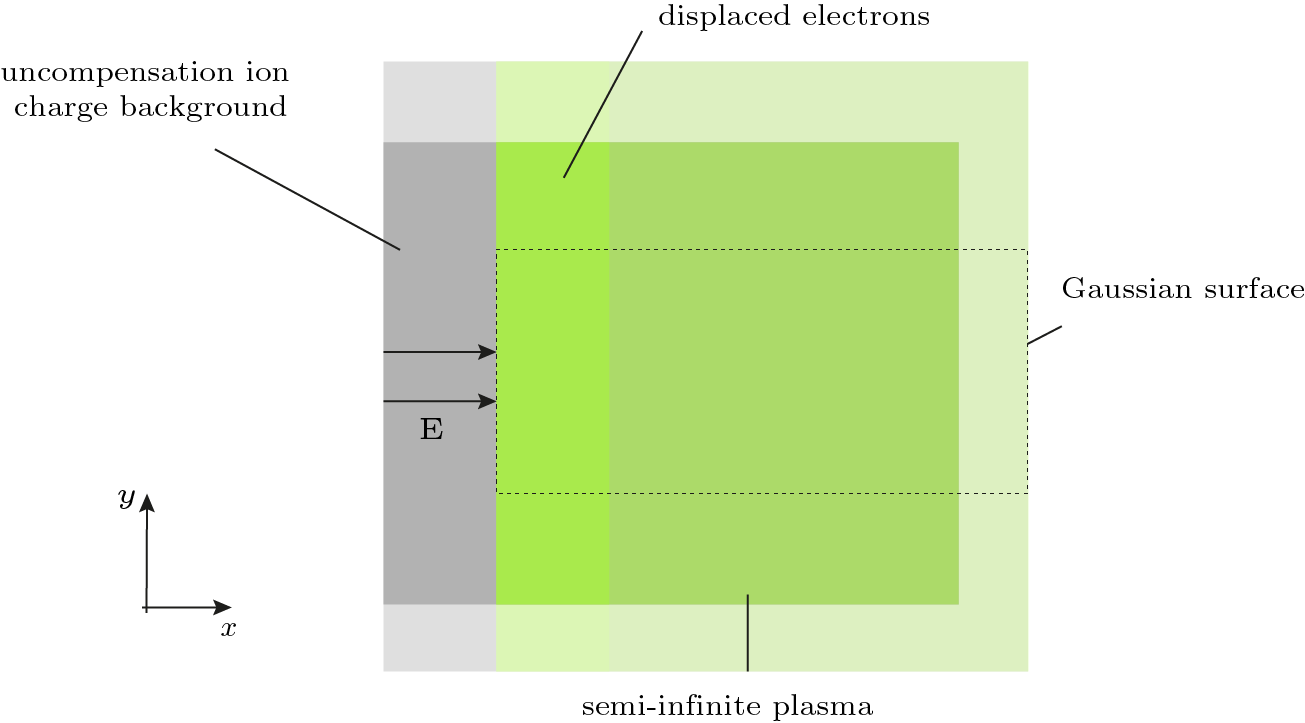
\includegraphics[width=0.7\linewidth]{figures/intro/intro_plasma_frequency}
	\caption[A diagram to illustrate the derivation of plasma frequency.]{\textbf{A diagram to illustrate the derivation of plasma frequency.} The electrons of a semi-infinite plasma are displaced inwards by some external force leaving in their wake an uncompensated space charge of `immobile' positive ions. By constructing a Gaussian surface along the dashed line, the electric field associated with the positive space charge can be calculated from Gauss' Law.}
	\label{fig:introplasmafrequency}
\end{figure}
The total charge of displaced electrons within a surface area of $\sigma$ is 
\begin{equation}\label{eq:intro_Q}
	Q = -en_\mathrm{e}\sigma\Delta x.
\end{equation}
Applying the integral form of Gauss' law (from equation \ref{eq:intro-E0}) to the surface described in Figure \ref{fig:introplasmafrequency}, the uncompensated charge leads to 
\begin{equation}\label{eq:intro_E}
	-\sigma E\hat{\mathbf{x}}= \frac{Q}{\epsilon_0}\hat{\mathbf{x}} = -\frac{en_\mathrm{e}\sigma\Delta x}{\epsilon_0}\hat{\mathbf{x}}
\end{equation}
at the plasma surface. By the Lorentz force, Equation \ref{eq:intro-Lorentz_force}, the displaced electrons will experience a restoring force, $-eE\hat{\mathbf{x}}$, perpendicular to the surface due to the electron-ion charge imbalance. The equation of motion for electrons on that surface is therefore
\begin{equation}\label{eq:intro_sho}
	m_e\frac{\mathrm{d}^2\Delta x}{\mathrm{d}t^2} = -eE = -\frac{e^2n_\mathrm{e}}{\epsilon_0}\Delta x.
\end{equation}
Equation \ref{eq:intro_sho} clearly describes a simple harmonic oscillator with a characteristic frequency given by the plasma frequency,
\begin{equation}
	\omega_\mathrm{p} = \sqrt{\frac{e^2n_\mathrm{e}}{m_\mathrm{e} \epsilon_0}}.
\end{equation}

% TODO Scheck's notes cover that the collisionality condition is always satisfied for a classical plasma (Archie Bott to send the notes)

\section{The Lawson-Woodward theorem}\label{sec:intro-lawson_woodward}
The Lawson-Woodward theorem states that there can be no net electron energy gain from laser fields \cite{esareyPhysicsLaserdrivenPlasmabased2009}, quite at odds with one of the primary aspects of this thesis, that is, the acceleration of electrons. There are, however, several conditions that are frequently met, namely,
\begin{enumerate}
	\item The interaction region is infinite.
	\item The interaction occurs in a vacuum.
	\item The electron is ultra-relativistic ($v\approx c$) along the acceleration gradient.
	\item No electro- or magnetostatic fields are present.
	\item Non-linear effects are neglected.
\end{enumerate}
Several of these apply to the various accelerations of electrons considered here. It is this final condition that is most damning to the application of the theorem. Throughout this thesis, the ultra-relativistic laser pulses under consideration ensure non-linear effects cannot be neglected. It is indeed such non-linearities that are of most interest.

\section{Laser-solid density plasma linear interaction}\label{sec:intro-lasersolidplasma_linear}
Consider small transverse electromagnetic waves propagating through a plasma. Linearising equation \ref{eq:intro-Lorentz_force} for a single plasma electron by assuming only small field variations and thus small velocity variation,
\begin{equation}\label{eq:intro-EOM_linear}
	m_\mathrm{e}  \dot{\mathbf{v}}_\mathrm{e} = -e\mathbf{E}.
\end{equation}
Combining the time derivative of Equation \ref{eq:intro-B1} and the curl of Equation \ref{eq:intro-E1},
\begin{equation}
	\nabla\times\nabla \times \mathbf{E}= - \mu_0 \dot{\mathbf{J} }- \mu_0\epsilon_0 \ddot{\mathbf{E}}.
\end{equation}
Considering only fast oscillations, such that ions are effectively immobile,
\begin{equation}
	\mathbf{J} = - n_\mathrm{e} e\mathbf{v}_\mathrm{e}
\end{equation}
and using the identity $\nabla\times\nabla \times \mathbf{E} = \nabla(\nabla\cdot \mathbf{E}) - \nabla^2\mathbf{E}$,
\begin{equation}
	\nabla(\nabla\cdot \mathbf{E}) - \nabla^2\mathbf{E} = -\frac{\mu_0 n_\mathrm{e} e^2}{m_\mathrm{e}} \mathbf{E}  - \mu_0 \epsilon_0 \ddot{\mathbf{E}}.
\end{equation} 
Assuming plane wave solutions of the form
\begin{equation}
	\mathbf{E} = \mathbf{E_0}e^{i(\mathbf{k}\cdot \mathbf{x}-\omega t)},
\end{equation}
where $\mathbf{k}$ is the wave-vector and $\omega$ the frequency of oscillations and noting the waves are transverse $\mathbf{k}\cdot \mathbf{E} = 0$,
\begin{equation}
	|\mathbf{k}|^2 \mathbf{E} = -\frac{\mu_0 n_\mathrm{e} e^2}{m_\mathrm{e}}\mathbf{E} + \mu_0\epsilon_0\omega^2\mathbf{E}
\end{equation}
and hence the dispersion relation for electromagnetic waves propagating in a plasma is
\begin{equation}\label{eq:intro-EM_dispersion}
	\omega^2  = c^2|\mathbf{k}|^2  + \omega_\mathrm{p}^2.
\end{equation}
Equation \ref{eq:intro-EM_dispersion} exhibits a \textit{cutoff} dependent on the plasma density via $\omega_\mathrm{p}$. The \textit{critical density}, $n_\mathrm{c}$, is defined as the density above which a laser pulse of frequency $\omega_\mathrm{L}$ cannot propagate through a plasma. This occurs for $\omega_\mathrm{L} = \omega_\mathrm{p}$, thus,
\begin{equation}
	n_\mathrm{c} = \frac{m_\mathrm{e}\epsilon_0 \omega_\mathrm{L}^2}{e^2}.
\end{equation}
As the plane wave has a spatial dependence $\sim \exp{(\mathbf{k}\cdot\mathbf{x})}$, if $n_\mathrm{e} > n_\mathrm{c}$, $\mathbf{k}$ is imaginary and the wave no longer propagates through the plasma and instead exponentially attenuates over a skin depth,
\begin{equation}
	\delta = \frac{1}{|\mathbf{k}|} = \frac{c}{\sqrt{\omega_\mathrm{p}^2 - \omega_\mathrm{L}^2}}
\end{equation}
and is reflected. For typical high-power lasers with wavelengths in the visible or near-infrared, fully ionised solids tend to have densities well above the critical density and thus produce plasma mirrors.

\section{Relativity}
Modern high-power lasers operate in the domain of relativistic mechanics and in general interactions are highly non-linear. It is useful to introduce some of the basic principles of relativity. There has been growing interest in the curvature of spacetime from relativistic lasers \cite{atongaGravitationalWavesHighpower2023}, however, this effect remains undetectable at present. Thus, throughout this thesis, the inner product of 4-tensors is defined using the Minkowski Metric \cite{steaneRelativityMadeRelatively2012}. 

Many useful quantities can be arranged into contravariant four-vectors that undergo a Lorentz transformation for a change of frame of reference \cite{steaneRelativityMadeRelatively2012}, specifically, 
\begin{equation}
	\mathbf{A}'^\mu =\Lambda_\mu^\nu \mathbf{A}^\mu,
\end{equation}
where $\Lambda^\mu_\nu$ is the appropriate Lorentz transformation, and primed symbols typically denote boosted frames of reference. Without loss of generality, the coordinate system can be defined such that the boosted frame travels along the $\mathbf{x}$-axis with respect to the initial frame. Thus, the Lorentz transformation is defined as
\begin{equation}\label{eq:zvp_lorentz}
	\Lambda_\mu^\nu = \begin{pmatrix}
		\gamma & -\beta\gamma & 0 & 0\\
		-\beta\gamma & \gamma & 0 & 0\\
		0 & 0& 1 & 0\\
		0 & 0 & 0 & 1
	\end{pmatrix}.
\end{equation}
Generally, a \textit{beta factor} is a normalised speed or velocity of an object,
\begin{equation}
	\beta = \frac{v}{c}, 
\end{equation}
here it refers to the frame velocity and its associated Lorentz or \textit{gamma factor} is
\begin{equation}
	\gamma = \frac{1}{\sqrt{1-\beta^2}}.
\end{equation}
Four-vectors relevant to this thesis are listed in Table \ref{tab:intro-four-vectors}.
%Many useful quantities can be arranged into contravariant four-vectors that undergo a Lorentz transformation for a change of frame of reference, those relevant to this thesis are: the four-displacement
%\begin{equation}
%	\mathbf{X}^\mu = (ct, \mathbf{x}),
%\end{equation}
%the four-potential
%\begin{equation}
%\mathbf{A}^\mu = \left(\frac{\phi}{c}, \mathbf{A}\right),
%\end{equation}
%the four-current density
%\begin{equation}
%	\mathbf{J}^\mu = (c\rho,\mathbf{J}),
%\end{equation}
%the four-wave vector
%\begin{equation}
%	\mathbf{K}^\mu = \left(\frac{\omega}{c}, \mathbf{k}\right)
%\end{equation}
%and the four-momentum of a particle
%\begin{equation}
%	\mathbf{P}^\mu = \left(\frac{U}{c}, \mathbf{p}\right),
%\end{equation}
%where $U = \gamma m c^2$ is the particle energy and $\mathbf{p} = \gamma m\mathbf{v}$ its three-momentum.
\begin{table}
	\begin{center}
		\begin{tabular}{llll}
			\hline \hline
			Symbol & Name & Components & Invariant \\
			\hline
			$\mathbf{X}^\mu$& 4-displacement & $(ct, \mathbf{x})$ & $-c^2\tau^2$  \\
			$\mathbf{A}^\mu$&4-potential  & $(\phi/c, \mathbf{A})$  &  \\
			$\mathbf{J}^\mu$& 4-current density & $(c\rho,\mathbf{J})$ & $-c^2\rho_0^2$ \\
			$\mathbf{K}^\mu$& 4-wave vector &$(\omega/c, \mathbf{K})$  &  \\
			$\mathbf{P}^\mu$& 4-momentum &  $(U/c, \mathbf{p})$& $-m^2c^2$ \\
			\hline \hline
		\end{tabular}
		\caption{\label{tab:intro-four-vectors} \textbf{Four-vectors of relevance to this thesis.} New parameters are the proper time, $\tau$, the proper charge density, $\rho_0$, energy, $U = \gamma m c^2$, three-momentum, $p = \gamma m\mathbf{v}$.}
	\end{center}
\end{table}
Transformations of electromagnetic fields under reference frame boosts are given in Appendix \ref{sec:app_lorentzEM}. Maxwell's equations are Lorentz covariant.
% TODO ensure all mentions of energy use U for bulk and T for individual

Focusing now on the 4-potential $\mathbf{A}^\mu$ and choosing the Lorenz gauge,
\begin{equation}
	\partial_\mu \mathbf{A}^\mu = \nabla \cdot \mathbf{A} + \frac{1}{c^2}\partial_t \phi = 0,
\end{equation}
then Maxwell's equations can be written
\begin{equation}\label{eq:intro-wave_equation}
	\partial_\nu \partial^\nu \mathbf{A}^\mu = -\frac{1}{c^2\epsilon_0}\mathbf{J}^\mu.
\end{equation}
Equation \ref{eq:intro-wave_equation} can be solved to yield 
\begin{equation}
	\mathbf{A}(\mathbf{x},t) = \frac{\mu_0}{4\pi} \int \frac{\mathbf{J}(\mathbf{x'},t_\mathrm{a})}{|\mathbf{x}-\mathbf{x}'|} \mathrm{d}^3\mathbf{x}',
\end{equation}
where $t_\mathrm{a} = t- |\mathbf{x}-\mathbf{x}'|/c$ is the advanced time. Hence, electromagnetic fields radiated from charged particles in motion can be calculated\footnote{Or even, as is performed in the full technical derivation relevant for the work of Chapter \ref{ch:3-orion}, electromagnetic fields can be described in terms of the future charge motions they will incite \cite{baevaHighHarmonicGeneration2008}.}.

% TODO I think this is a good spot for the relativistic Larmor frequency

\subsection{Ultra-relativistic similarity theory}
Consider a relativistically intense laser pulse normally incident on a collisionless plasma as in Figure \ref{fig:introplasmafrequency}. Again neglect ion motion. The electron distribution is fully described by the Vlasov equation (Equation \ref{eq:intro-vlasov}) with the self-consistent electric and magnetic fields satisfying Maxwell's equations (Equations \ref{eq:intro-maxwell}). Suppose the incident laser pulse has an initial vector potential 
\begin{equation}
	\mathbf{A}(t=0) = \mathbf{a}((y^2+z^2)/R^2,x/c\tau)\cos k_\mathrm{L}x.
\end{equation}
This envelope form for the potential, $\mathbf{a}((y^2+z^2)/R^2,x/c\tau)$, is sensible provided $k_\mathrm{L}R \gg 1$ and $\omega_\mathrm{L}\tau \gg 1$, where $R$ is the focal spot radius and $\tau$ the pulse duration. For fixed laser envelope, the laser-plasma dynamics depend on just four dimensionless variables:  the normalised focal spot size, $k_\mathrm{L} R$, the normalised pulse duration, $\omega_\mathrm{L}\tau$, the normalised laser vector potential amplitude
\begin{equation}
	a = \mathrm{max}\left|\frac{e \mathbf{A} }{m_\mathrm{e} c^2 }\right|,
\end{equation}
in terms of the peak laser electric field amplitude $\mathbf{E}_\mathrm{L}$,
\begin{equation}
	a_0 = \frac{e|\mathbf{E}_\mathrm{L}|}{m_\mathrm{e} c\omega_\mathrm{L}},
\end{equation}
and the normalised plasma density
\begin{equation}
	\bar{n}_\mathrm{e} = \frac{n_\mathrm{e}}{n_\mathrm{c}}.
\end{equation}
By normalising the system of equations and combining these last two expressions into the \textit{relativistic similarity parameter},
\begin{equation}
	S = \frac{\bar{n}_\mathrm{e}}{a_0},
\end{equation}
it is possible to show that in the ultra-relativistic limit ($a_0 \gg 1$), the dynamics of the system are similar for constant $S$ \cite{gordienkoScalingsUltrarelativisticLaser2005} with plasma electrons following similar trajectories where 
\begin{equation}\label{eq:intro-p_similarity}
	\mathbf{p} \sim a_0.
\end{equation}
There is also a more physical meaning to the $S$ parameter. Consider again Section \ref{sec:intro-lasersolidplasma_linear} on the propagation of linear electromagnetic waves through a plasma but now for the case of an ultra-relativistic laser pulse. For an electron rotating in an electromagnetic field,
\begin{equation}
	\mathbf{F}_\perp = \gamma m_e \mathbf{a}_\perp,
\end{equation}
where $ \mathbf{a}_\perp$ is the acceleration perpendicular to the motion and thus the response of the electrons is reduced by a factor of $\gamma$. While some find the \textit{relativistic mass} correction to be somewhat unhelpful nomenclature for the phenomenon \cite{steaneRelativityMadeRelatively2012}, it has nevertheless become commonplace within the literature of relativistic plasma physics \cite{umstadterRelativisticLaserPlasma2003}. Turning the handle, one finds that the relativistic plasma frequency is
\begin{equation}
	\omega_\mathrm{p}^\mathrm{rel} = \sqrt{\frac{e^2n_\mathrm{e}}{\gamma m_\mathrm{e} \epsilon_0}}.
\end{equation}
Using equation \ref{eq:intro-p_similarity}, and taking $v \approx c$, then $\gamma \approx a_0$ and the normalised relativistic cutoff density is simply $S$. Thus, the ultra-relativistic similarity parameter is simply a measure of the overdensity of a plasma once relativistic corrections have been applied, \textit{i.e.} for $S>1$, a laser pulse will be reflected, however for $\bar{n}_\mathrm{e} > 1$ and $S <1$, one enters the regime of relativistically self-induced transparency \cite{ereminRelativisticSelfInducedTransparency2010}. It is now possible to define the parameter space of interest in this thesis: relativistic laser-plasma surface interactions occur for $a_0 \gg 1$ and $S > 1$.

\subsection{Relativistic lasers and plasmas}
The descriptor \textit{relativistic} is applied liberally in this thesis. When applied to electromagnetic fields or laser pulses it refers to 
\begin{equation}
	a_0 \ge 1.
\end{equation}
When applied to particles, their Lorentz factors are
\begin{equation}
	\gamma = \frac{1}{\sqrt{1-\beta^2}} \ge 2,
\end{equation}
corresponding to a speed, $u \ge 0.87 c$. \textit{Ultra-relativistic} implies these quantities are much larger than the conditions provided. A relativistic laser pulse will accelerate electrons to relativistic velocities in a fraction of a laser pulse cycle. Consider an electron in the presence of a uniform electric field of magnitude $a_0 = 100$, an intensity accessible by current state-of-the-art laser facilities. The work done on that particle by the field is 
\begin{equation}
	T = (\gamma -1)m_\mathrm{e}c^2 = \int \mathbf{E}\cdot \mathrm{d} \mathbf{x},
\end{equation}
The field will accelerate an electron to relativistic velocities in a distance less than 1 \% of a corresponding laser pulse wavelength. It is reasonable therefore to assume the interaction is instantaneously relativistic.

Upon entrance to the relativistic regime, the motion of an electron fundamentally changes. Consider Equation \ref{eq:intro-Lorentz_force}. For non-relativistic laser pulses, the magnetic field component can be neglected and the electron simply oscillates along the electric field vector direction. Once electron velocities approach $c$, this approximation is no longer valid. Electrons are rotated in the magnetic field and accelerated along the laser propagation direction. In a plasma, this enables inwards compression of the surface, leading to laser-induced hole boring \cite{wilksAbsorptionUltraIntenseLaser1992}.

\subsection{Conservation of generalised transverse momentum}\label{sec:intro_conservation-generalised-mometum}
Consider a holonomic system of $N$ relativistic particles under the influence of electromagnetic forces. A particle $j$ with charge $e_j$ and mass $m_j$ experiences a scalar potential,
\begin{equation}
	V_{j} = e_j(\phi - \mathbf{A} \cdot \mathbf{v}_{j})
\end{equation}
and hence the system is described by the Lagrangian \cite{goldsteinClassicalMechanics2013}
\begin{equation}
	\mathcal{L} = \sum^N_{j=1}\left( - m_jc^2\sqrt{1-\beta^2_\mathrm{j}} - e_j(\phi - \mathbf{A} \cdot \mathbf{v}_j) \right),
\end{equation}
The generalised momentum corresponding to coordinate $x_j$ is
\begin{equation}
	p_{j,x} = \frac{\partial L}{\partial \dot{x}_j} = \frac{m_j\dot{x}_j }{\gamma_j}+ e_jA_x,
\end{equation}
describing both the linear mechanical momentum and the momentum of the electromagnetic field. Via Noether's theorem, if $L$ is independent of $x_j$, \textit{i.e.} spatially homogeneous along $x$ for particle $j$, then 
\begin{equation}\label{eq:intro-transverse_momentum_differential_equation}
	\dot{p}_{j,x} = 0
\end{equation}
since
\begin{equation}
	\frac{\mathrm{d}}{\mathrm{d}t}\left(\frac{\partial L}{\partial \dot{x}_j}\right) = \frac{\partial L}{\partial x_j}.
\end{equation}

Taking the Lorenz gauge, consider a linearly polarised Gaussian laser pulse, with an axis of polarisation along $x$ incident on a solid target at rest. Then $A_x$ is approximately constant along $x$ near the beam centre\footnote{Constant relative to the scale of typical electron trajectories in such an interaction.}. Integrating Equation \ref{eq:intro-transverse_momentum_differential_equation}, fully constraining the gauge by setting the potential to zero initially, and noting that there is no linear momentum at the target, the generalised transverse momentum conservation equation for an electron in the laser field is
\begin{equation}\label{eq:intro-transverse_momentum_conservation_no_initial_momentum}
	p_\mathrm{T} = eA,
\end{equation}
where $p_\mathrm{T}$ is the electron momentum along the polarisation axis of the laser pulse and $A$ is the laser pulse 3-vector potential amplitude. As a sanity check, this expression complies with the ultra-relativistic similarity result of Equation \ref{eq:intro-p_similarity}.
% TODO note that setting the boundary conditions is the final requirement to fix the gauge in the Lorenz gauge formalism.

Note that this is only valid provided the electron does not radiate along the direction of polarisation as discussed by Sokolov \textit{et al} \cite{sokolovDynamicsEmittingElectrons2009}. The implications of \textit{Radiation Reaction }are discussed in the following section.

\section{QED effects}
% TODO cite Schwinger limit
Next-generation laser facilities will enable the testing of decades-old theoretical predictions of \ac{SF-QED}. Already Fedeli \textit{et al} have shown in simulations that current PW-class laser facilities can access this regime using an all-optical set-up based on laser-solid surface interactions \cite{fedeliProbingStrongfieldQED2020}. The Schwinger Limit $E_\mathrm{S} = \qty{1.32e18}{V.m^{-1}}$ is the field intensity at which the vacuum non-linearity can produce real particles. If by some means an electron can be directed towards a plane electromagnetic wave, by consideration of the Lorentz transformations of electromagnetic fields (equations \ref{eq:app-maxwell_transformation}), it is possible that provided the electron is sufficiently relativistic, in its own reference frame it will `see' electromagnetic fields intense enough to access such vacuum non-linearities. The first two frontiers of SF-QED that will be accessed are Radiation Reaction and multi-photon Breit-Wheeler electron pair production. Brief introductions to these phenomena are now presented.

\subsection{High-energy photon emission and radiation reaction}
When a charged particle undergoes an acceleration, it emits electromagnetic radiation. If the electromagnetic field is sufficiently strong, \textit{i.e.} approaching the Schwinger Limit in the rest frame of the particle, then a non-negligible fraction of the particle momentum can be transferred to the emitted high energy photon, substantially impacting the dynamics of the accelerated particle. This back reaction is known as \ac{RR}.

Smilei (detailed in the following section) implements the process of high-energy photon emission as Inverse Compton Scattering on the basis of several assumptions \cite{nielQuantumClassicalModeling2018}, namely,
\begin{enumerate}
	\item Radiating particles are ultra-relativistic and therefore radiation is emitted in the direction of travel of the particle.
	\item The field varies slowly over the timescale of photon emission, this is the \textit{locally-constant field approximation} and requires ultra-relativistic field strengths;
	\item but they are small with respect to the Schwinger Limit, specifically requiring the invariants $\sqrt{c^2\mathbf{B^2} + \mathbf{E}^2}$ and $\sqrt{c\mathbf{B}\cdot\mathbf{E}} < E_\mathrm{S}$.
	\item Real particles radiate independently of their neighbours, this requires the emitted wavelength to be shorter than the typical inter-particle spacing.
\end{enumerate}
Provided such conditions hold, the rate of photon emission depends on two invariants \cite{ritusQuantumEffectsInteraction1985}, the electron quantum parameter
\begin{equation}
	\chi = \frac{\gamma}{E_\mathrm{S}}\sqrt{(\mathbf{E} + \mathbf{v}\times\mathbf{B})^2- (\mathbf{v}\cdot\mathbf{E})^2/c^2},
\end{equation}
where $\mathbf{v}$ is the electron velocity and the emitted photon quantum parameter
\begin{equation}\label{eq:intro-photonchi}
	\chi_\gamma = \frac{\gamma_\gamma}{E_\mathrm{S}}\sqrt{(\mathbf{E}_\perp + \mathbf{c}\times\mathbf{B})^2- (\mathbf{c}\cdot\mathbf{E})^2/c^2},
\end{equation}
where $\gamma_\gamma$ is the normalised photon energy $=\hbar \omega_\gamma /m_\mathrm{e}c^2$. The exact relationship is complex and in the fully quantum domain ($\chi > 1$), is it not practical to solve the integrations required for all particles. Instead, values are extracted from precalculated tables and supplied to a Monte Carlo algorithm. 

\subsection{Multi-photon Breit-Wheeler pair production}
Multi-photon Breit-Wheeler pair production, also known as non-linear Breit-Wheeler is the decay of a high energy photon, typically produced via \ac{RR}, into an electron-positron pair in the presence of a strong electromagnetic field, explicitly,
\begin{equation}
	\gamma + n\omega \to e^- + e^+.
\end{equation}
The strength of the effect is dependent on the Lorentz invariant photon quantum parameter, Equation \ref{eq:intro-photonchi}. In a constant electric field, the rate of pair production increases rapidly up to $\chi_\gamma \approx 10$ at which point it saturates and slowly reduces.

% TODO \textbf{Perhaps include Feynmann diagrams, see what Savin did.}

\section{Simulating the interaction}
Modelling laser-plasma interactions is a notoriously challenging endeavour. Due to the complexity of the many-bodied systems involved (a fully ionised centimetre cubed block of plastic contains on the order of $10^23$ particles) and the stochasticity of particle motion, it is frequently impossible to construct models \textit{ab initio}. Instead, hydrodynamic simulation codes such as HYADES \cite{larsenHYADESPlasmaHydrodynamics1994} and FLASH \cite{fryxellFLASHAdaptiveMesh2000} and Particle-In-Cell simulation codes such as Smilei \cite{derouillatSmileiCollaborativeOpensource2018}, Osiris \cite{fonsecaOSIRISThreeDimensionalFully2002} and EPOCH \cite{bennett2017users} are used to construct phenomenological models and to direct experimentation. 

\subsection{Supercomputing resources}\label{sec:intro-archer}
Modern \ac{HPC} systems are poised to enter the exascale regime ($> 10^{18}$ Floating Point Operations Per Second). With limited improvements in microprocessor technologies, such power is achieved through massive parallelisation across processing units. Able to study the dynamics of billions of macroparticles, PIC codes test the limits of modern supercomputing architectures. ARCHER2, the UK's national supercomputer, came online in November 2021, with it delivering over ten times the resources of its predecessor (ARCHER) \cite{ARCHER2}. An HPE Cray EX supercomputing system with a peak performance estimated at \qty{28}{Pflops.s^{-1}} across 5860 nodes each with dual AMD EPYCTM 7742 64-core processor for a total of 750,080 cores, ARCHER2 was able to supply the resources required to run the costly PIC simulations for this research. The substantially cheaper HYADES simulations were performed on the Rutherford Appleton Laboratory's SCARF \ac{HPC} cluster \cite{SCARFOverview}.

\subsection{Particle-In-Cell codes}

\subsubsection{Discretisation of the Vlasov-Maxwell equations}
Finding numerical solutions to the Vlasov-Maxwell equations is no straightforward. While codes exist that are capable, such as Valis \cite{sircombeVALISSplitconservativeScheme2009}, the requirement of high resolution in both position and momentum is exceedingly costly and the use of such codes is limited with respect to their size, duration and number of spatial dimensions. A more tractable approach is to discretise the distribution function into $N_s$ \textit{quasi-particles}\footnote{Originally introduced by Langdon and Birdsall as \textit{clouds} \cite{langdonTheoryPlasmaSimulation1970}.}. These are often referred to as \textit{macro-particles} in practice and typically represent a large number of real particles, such that
\begin{equation}
	f_s(t,\mathbf{x},\mathbf{p}) = \sum^{N_s}_{p=1} w_p S(\mathbf{x}-\mathbf{x}_p(t))\delta (\mathbf{p}-\mathbf{p}_p(t)),
\end{equation}
where $w_p$ is the quasi-particle's weight, $\mathbf{x}_p$ and $\mathbf{p}_p$ are its position and momentum respectively, $\delta$ is the Dirac-delta distribution and $S(\mathbf{x})$ the shape-function chosen to represent the spatial extent of the quasi-particle. The Vlasov equation is then integrated along the continuous trajectories of quasi-particles while Maxwell's equations are solved on a discrete spatial grid of \textit{cells}. Such a code is aptly named a \textit{Particle-In-Cell} (PIC) code. A schematic of the standard PIC code algorithm is presented in Figure \ref{fig:intropiccycle-01}. 
\begin{figure}
	\centering
	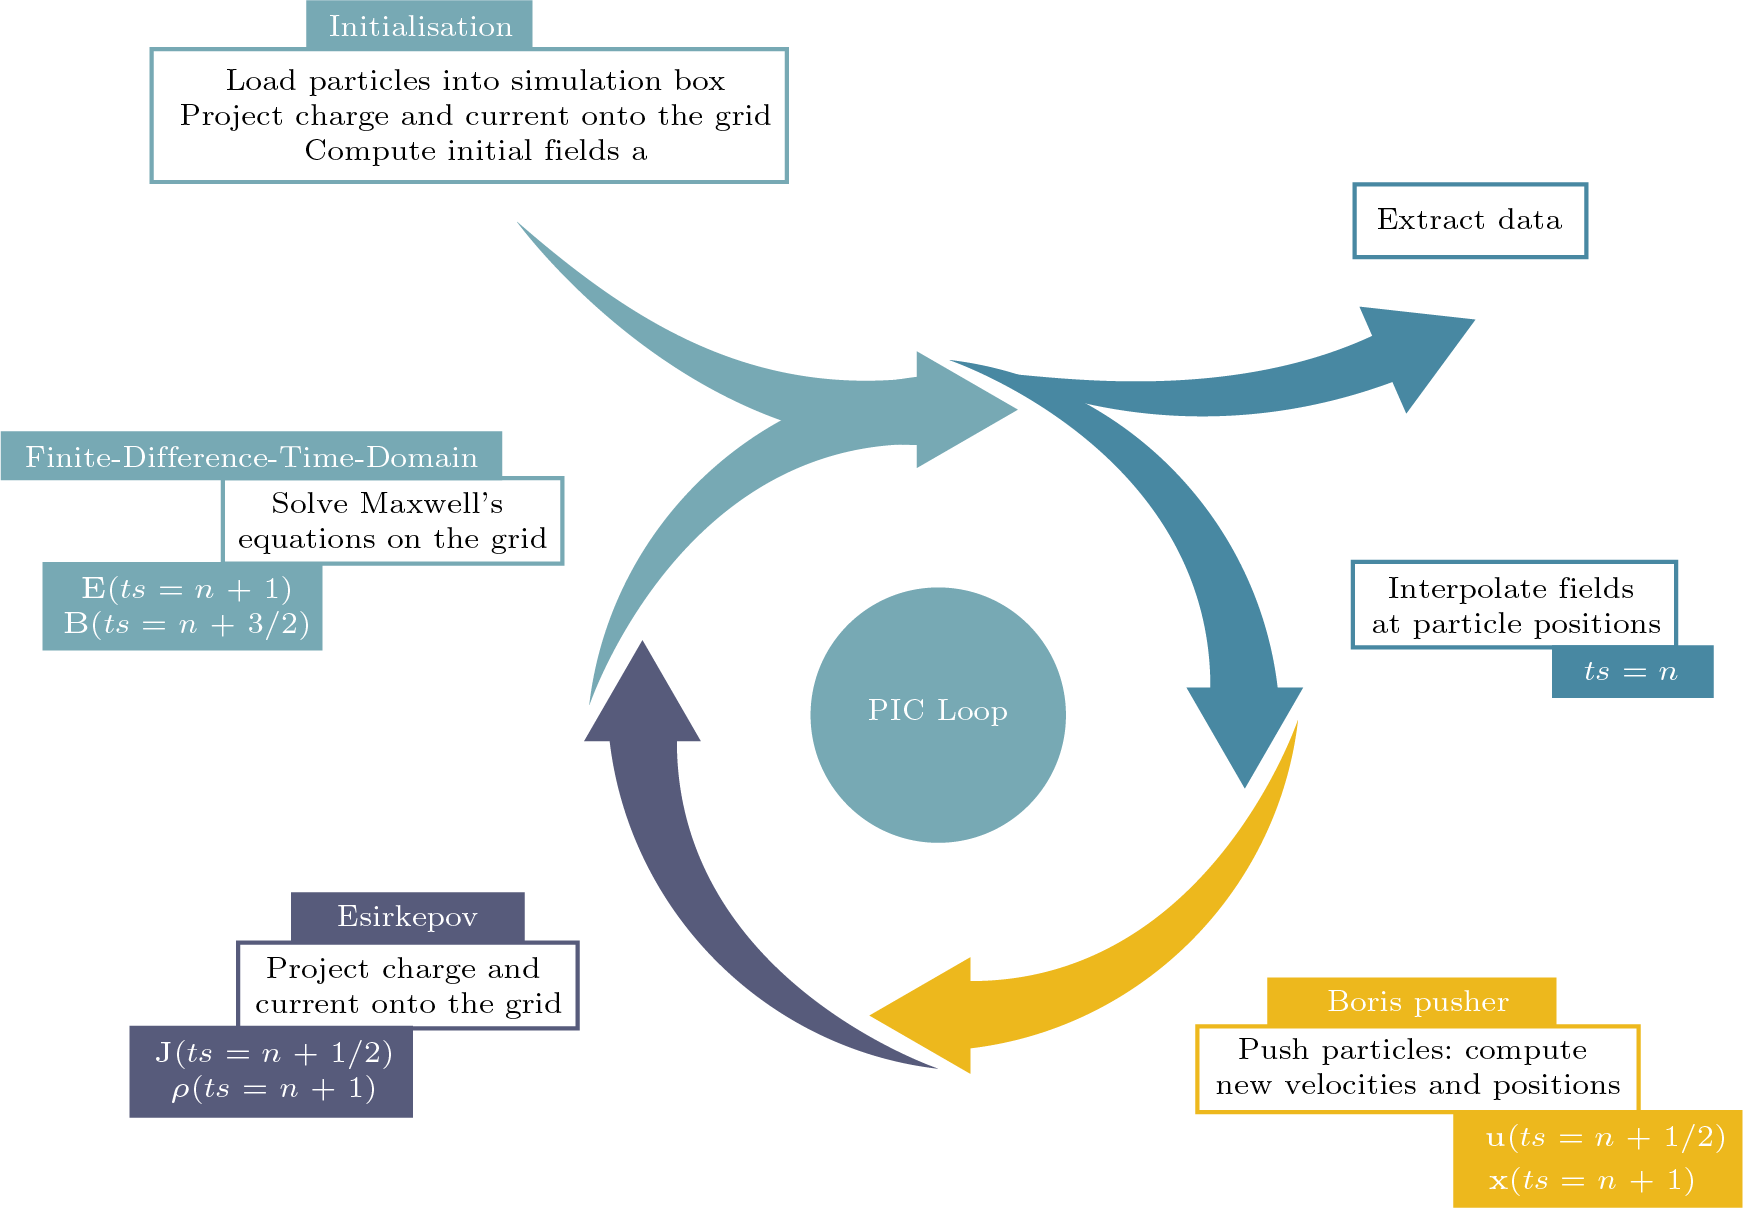
\includegraphics[width=\linewidth]{figures/intro/intro_PIC_cycle}
	\caption[A schematic of the PIC code loop and the algorithms performed.]{A schematic of the PIC code loop and the algorithms performed from time step, $ts$, from $n$ to $n+1$.}
	\label{fig:intropiccycle-01}
\end{figure}
After particle and field initialisation, fields are interpolated at particle positions. The well-established momentum-conserving \textit{Boris pusher} algorithm computes the new macro-particle velocities and positions \cite{borisRelativisticPlasmaSimulationoptimization1970}. Particles are advanced in time using a \textit{leap-frog }scheme, where positions are defined at integer, $n$, time steps and momenta at half-integer, $n + 1/2$. The charge conserving Esirkepov algorithm \cite{esirkepovExactChargeConservation2001} projects the new charge and current densities onto the grid to then solve Maxwell's equations using the Finite-Difference-Time-Domain approach \cite{tafloveComputationalElectromagneticsFiniteDifference2005}. To ensure space and time centring of the electromagnetic field derivatives in Maxwell's equations, electric and magnetic fields are discretised on the staggered \textit{Yee grid} as represented in Figure \ref{fig:introyeegrid}. 
\begin{figure}
	\centering
	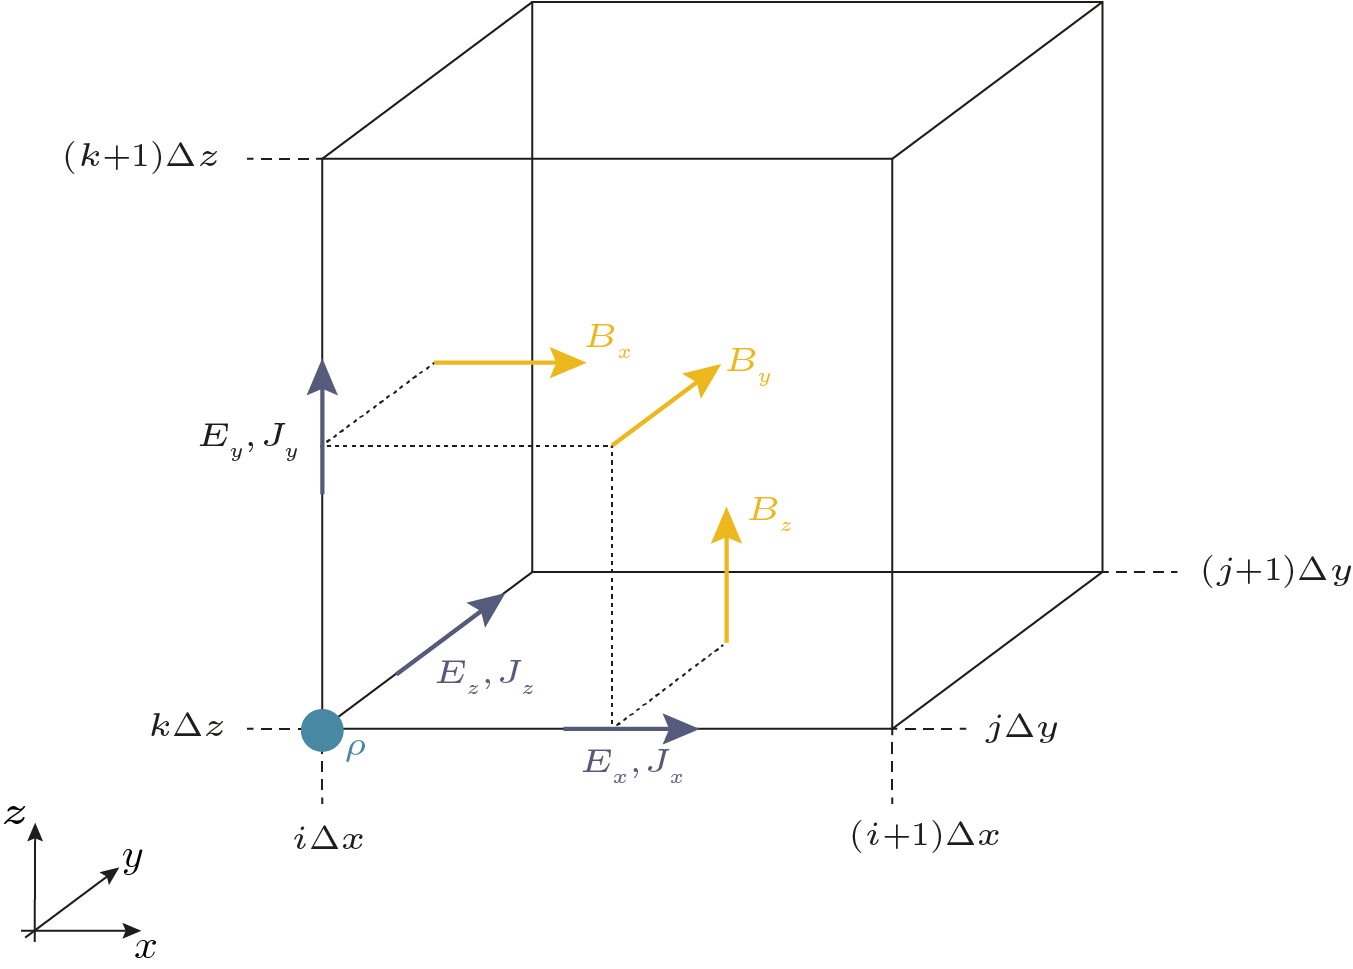
\includegraphics[width=0.7\linewidth]{figures/intro/intro_yee_grid}
	\caption[A representation of the staggered Yee grid.]{\textbf{A representation of the staggered 3D Yee grid.} For the cell at $(i\Delta x, j\Delta y, k\Delta z)$ for spatial centring of the curl operations, including the locations where all system properties are defined.}
	\label{fig:introyeegrid}
\end{figure}
with electric fields defined at integer time steps and magnetic fields at half-integer time steps.

\subsubsection{Smilei}
Smilei (for Simulating Matter Irradiated by Light at Extreme Intensities) is a modern, collaborative, massively parallel, fully relativistic and open source plasma physics PIC code and the major workhorse for this thesis\footnote{At points benchmarks against the EPOCH and Osiris PIC codes were performed.}. 
Produced at École Polytechnique, Paris \cite{derouillatSmileiCollaborativeOpensource2018}, its recent development was motivated by the recent advancements of multi-petawatt facilities both globally and locally with the completion in 2020 of the 10 PW Apollon laser facility and by the availability of supercomputing power which has `skyrocketed' in recent years \cite{derouillatSmileiCollaborativeOpensource2018}. The 3D \ac{PIC} simulations examined in this thesis demanded the parallelisation of almost 20 \% of the computing resources available on the ARCHER2 supercomputer.

\subsubsection{Reference units}
Given the broad range of magnitudes linked to multi-petawatt and femtosecond laser pulses, solid density plasmas, micrometre wavelengths, and attosecond electron bunches, it becomes significantly more convenient to transform them into dimensionless and normalised values. Smilei operates in such units. This normalisation is not chosen \textit{a priori}, instead results can be scaled by an arbitrary reference angular frequency. This is extremely useful when working with boosted frames of reference. As this thesis focuses on the interaction of a laser pulse with plasma, the laser pulse angular frequency, $\omega_\mathrm{L}$ is set as the frequency of reference. A list of the most common normalisations is provided in Table \ref{tab:intro-normalisations}.

\begin{table}
	\begin{center}
		\begin{tabular}{ccc}
			\hline \hline
			Units of & SI units & Normalisation \\
			\hline
			velocity & \unit{m.s^{-1}} & $c$ \\
			charge & C & $e$ \\
			mass & kg & $m_\mathrm{e}$ \\
			momentum & \unit{kg.m.s^{-1}} & $m_\mathrm{e}c$ \\
			energy/temperature & J & $m_\mathrm{e}c^2$ \\
			time & s & $\omega^{-1}_\mathrm{L}$ \\
			length & m & $c/\omega_\mathrm{L}$ \\
			number density & \unit{m^{-3}} & $n_\mathrm{c}$ \\
			electric field & \unit{V.m^{-1}} & $m_\mathrm{e}c\omega_\mathrm{L}/e$ \\
			\hline \hline
		\end{tabular}
		\caption{\label{tab:intro-normalisations} \textbf{Smilei normalisations for common quantities.} The laser angular frequency $\omega_\mathrm{L}$ is set at the reference angular frequency.}
	\end{center}
\end{table}

\subsubsection{Simulation parameters}\label{sec:intro-general_simulation_paramers}
\textit{Silver-M$\ddot{u}$ller} boundary conditions, chosen for the simulation box edges \cite{barucqAsymptoticBehaviorSolutions1997}, absorb and inject electromagnetic waves and particles. There can be non-physical reflection of electromagnetic waves at such boundaries leading to some error.

The quasi-particle shape function $S(\mathbf{x})$ determines the projection of particle charge onto the grid. It is symmetric in all dimensions with respect to $\mathbf{x}$ and extends over $n$ cells of width $\Delta x$ in each direction where $n$ is the interpolation order. It can be written as a product across $D$ dimensions,
\begin{equation}
	S(\mathbf{x}) = \Pi^D_{\mu = 1}s^{(n)}(x^\mu).
\end{equation}
Smilei implements orders 2, 3 and 4, the explicit shape functions are
\begin{subequations}
	\begin{align}
		s^2 (n) &= \begin{cases}
			\frac{1}{\Delta x}\left(1-\left|\frac{x}{\Delta x}\right| \right)  & \text{if } |x| \le \Delta x, \\
			0  & \text{otherwise,}
		\end{cases} \\
		s^3(n) &= \begin{cases}
			\frac{3}{4\Delta x}\left(1-\frac{4}{3}\left(\frac{x}{\Delta x}\right)^2 \right)  & \text{if } |x| \le \frac{1}{2}\Delta x, \\
			\frac{9}{8\Delta x}\left(1-\frac{2}{3}\left|\frac{x}{\Delta x}\right| \right)^2  & \text{if } \frac{1}{2}\Delta x <|x| \le \frac{3}{2} \Delta x, \\
			0  & \text{otherwise,}
		\end{cases}  \\
		s^4(n) &= \begin{cases}
			\frac{2}{3 \Delta x}\left( 1-\frac{3}{2}\left(\frac{x}{\Delta x}\right)^2 + \frac{3}{4}\left| \frac{x}{\Delta x}\right| ^3 \right)  & \text{if } |x| \le \Delta x, \\
			\frac{4}{3 \Delta x}\left(1-\frac{1}{2}\left|\frac{x}{\Delta x}\right| ^3 \right)  & \text{if } \Delta x <|x| \le 2\Delta x, \\
			0  & \text{otherwise.}
		\end{cases} 
	\end{align}
\end{subequations}

While the correct implementation of collisions in PIC codes remains an open problem \cite{Collisions}, Smilei has implemented relativistic binary collisions between macroparticles using a Monte-Carlo-based scheme \cite{perezImprovedModelingRelativistic2012}. The aforementioned QED processes of Inverse Compton scattering and non-linear Breit-Wheeler pair production are included using the built-in Smilei packages \cite{derouillatSmileiCollaborativeOpensource2018}. These processes can lead to cascades of many particles being added to the simulations. Macroparticle merging can increase simulation efficiency and reduce the memory footprint. Smilei implements such a scheme, inspired by that designed by Vranic \textit{et al} \cite{vranicParticleMergingAlgorithm2015}, that is computationally efficient and conserves energy, momentum and charge within a cell. While Smilei contains modules to handle ionisation, these are deemed unnecessary for the laser intensities considered in this thesis, as highlighted by Figure \ref{fig:intro_lasersystems}.

\subsubsection{Parallelisation in practice}
In the following discussion, where differences in language occur, objects are given their ARCHER2 (Smilei) names. The Smilei simulation box consists of a grid of cells as in Figure \ref{fig:introsmileiparallelisation}.
\begin{figure}
	\centering
	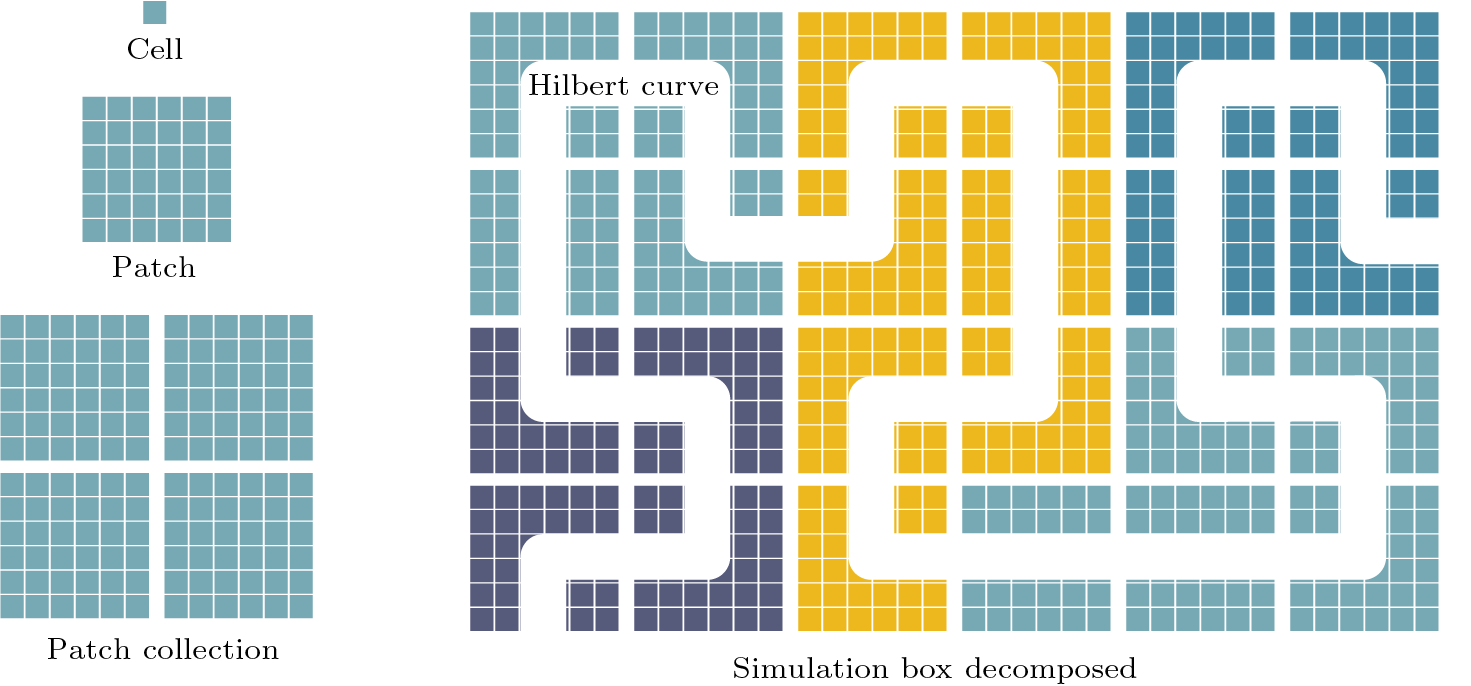
\includegraphics[width=1\linewidth]{figures/intro/intro_smilei_parallelisation}
	\caption[Smilei simulation box decomposition into cells, patches and MPI patch collections.]{\textbf{Smilei simulation box decomposition into cells, patches and MPI patch collections.} Cells are grouped into patches, patches are grouped into MPI patch collections. These collections are assigned patches contiguously along the Hilbert curve.}
	\label{fig:introsmileiparallelisation}
\end{figure}
The box is decomposed into \textit{patches} consisting of many cells. Patches are arranged into \textit{MPI patch collections} assigned contiguously along a Hilbert curve.

Archer consists of many \textit{CPUs (cores)} that can each perform computational tasks. CPUs are grouped into \textit{nodes}. Memory is shared within a node such that all CPUs (cores) in a node can operate on the same data. When optimised, ARCHER2’s memory in each node is split into 8 \textit{sockets}. These 8 sockets each perform a \textit{task (MPI process)}. Each task (MPI process) has 16 CPUs (cores) assigned that each perform a \textit{thread}. A thread is a sequence of instructions from the program.

Each task (MPI process) handles one \textit{MPI patch collection}. Threads work through patches. Figure \ref{fig:introsmileiparallelisationcomplex} represents this division of labour.
\begin{figure}
	\centering
	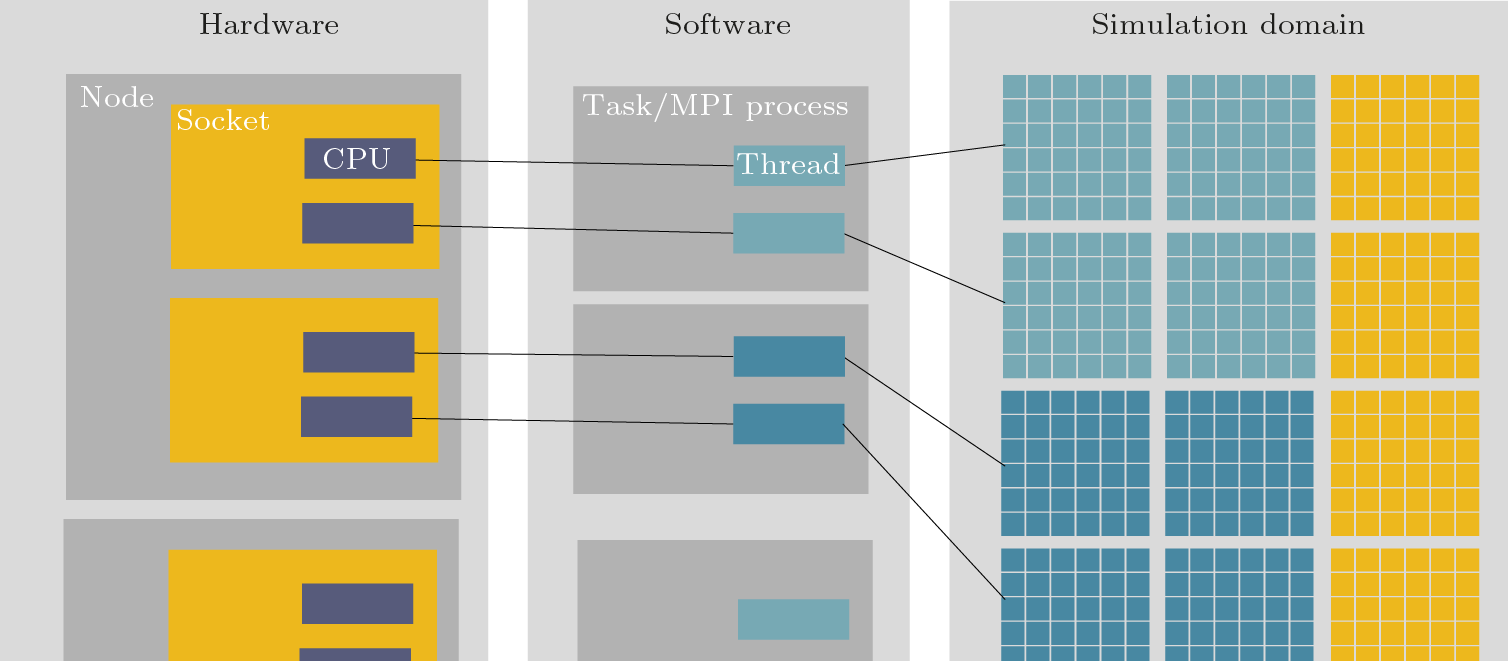
\includegraphics[width=1\linewidth]{figures/intro/intro_smilei_parallelisation_complex}
	\caption[Representation of the interaction of the ARCHER2 hardware and software components when running Smilei.]{\textbf{Representation of the interaction of the ARCHER2 hardware and software components when running Smilei. Each CPU is assigned a thread, each task is carried out by one socket. A task tackles one MPI patch collection with threads working through patches.}}
		\label{fig:introsmileiparallelisationcomplex}
\end{figure}
Threads do not need to wait for other threads in their process to tackle new patches in their MPI patch collection. This is a form of local \textit{dynamic load balancing}. If an MPI patch collection is overloaded, a patch is offloaded to a contiguous MPI patch collection.

There are several considerations for simulation optimisation. Tasks (MPI processes) should always be assigned more patches than threads. To apply the Hilbert curve, the number of patches in each dimension must be a power of 2. The fewer cells in a patch, the more efficient the load balancing, however, the cost of synchronisation between patches increases, although generally the gain in efficiency from load balancing by increasing patch number will win out at later times with increasing efficiency for increased frequency of load balancing \cite{derouillatSmileiCollaborativeOpensource2018}. Note that smaller patches are preferable when there are small regions with large numbers of particles, as in laser-solid surface interactions, however, the minimum patch size is dependent on the shape function of the macro-particles.

\subsubsection{Sources of error inherent to PIC codes}
Despite their relatively intuitive interpretation, PIC codes are famously finickety and prone to errors, most notably that of numerical self heating\footnote{Standard PIC code algorithms are charge and momentum conserving but not energy conserving \cite{derouillatSmileiCollaborativeOpensource2018}.}.

To ensure stability, or at least to minimise instability, there are several conditions which must be met. Naturally, the time step, $\Delta t$, and cell size ($\Delta x$x$\Delta y$x$\Delta z$) must adequately capture all interesting features of a given simulation. Typically such features are plasma wave oscillations,
\begin{equation}
	\Delta t \omega_\mathrm{p} \ll 1,
\end{equation} 
and laser pulse electromagnetic field oscillations or higher order harmonics of the laser pulse if that is of interest, for the $n$th harmonic
\begin{equation}
	\Delta t\omega_\mathrm{L}n \ll 1.
\end{equation} 
Note this also ensures that macroparticles are smaller than the wavelengths of the system, a requirement to ensure they mimic real particles \cite{okudaCollisionsPlasmaFiniteSize1970}. Relativistic PIC codes must satisfy the much-acclaimed \cite{demouraCourantFriedrichsLewy2013} Courant-Friedrichs-Lewy condition,
\begin{equation}
	\frac{1}{c\Delta t} > \sqrt{\frac{1}{(\Delta x)^2}+\frac{1}{(\Delta y)^2}+\frac{1}{(\Delta z)^2}},
\end{equation}
thus preventing light and relativistic particles from crossing a cell in one timestep and generating numerical Cerenkov radiation \cite{birdsall2004plasma}. As with real plasmas and real particles, to avoid numerical charge fluctuation and ensure the collective behaviour of macroparticles,
\begin{equation}
	\frac{4}{3}\pi\lambda_\mathrm{D}^3n_\mathrm{macro} = N_\mathrm{D,macro} \ggg 1,
\end{equation}
where $n_\mathrm{macro}$ is the macroparticle density \cite{birdsall2004plasma}. To avoid numerical heating, the cell size must resolve the Debye length,
\begin{equation}
	\frac{\lambda_\mathrm{D}}{\Delta x} \ge 1,
\end{equation}
failure to do so may cause plasma self-heating until the Debye length matches the cell size \cite{birdsall2004plasma}. Interestingly, Brackbill \textit{et al} \cite{brackbillEnergyMomentumConservation2016} observed in their simulations that setting $\lambda_\mathrm{D}/\Delta x =1$ was most effective at reducing spurious heating. Arber \textit{et al} \cite{arberContemporaryParticleincellApproach2015} performed extensive simulations exploring this instability. If the Debye length is not resolved, after an initial period of rapid self-heating, the temperature increases linearly and can be modelled as
\begin{equation}\label{eq:intro-selfheating}
	\frac{\mathrm{d} T_\mathrm{eV}}{\mathrm{d}t_\mathrm{ps}} = \alpha_\mathrm{H} \frac{n^{3/2}_{23} \Delta x^2_\mathrm{nm}}{N_\mathrm{ppc}},
\end{equation}
where $T_\mathrm{eV}$ is the temperature in electron volts, $t_\mathrm{ps}$ is the time in picoseconds, $n$ is the plasma electron number density in units of $10^{23}$ \unit{cm^{-3}}, $\Delta x_\mathrm{nm}$ is the cell size in nanometres and $N_\mathrm{ppc}$ is the number of macroparticles per cell with $\alpha_\mathrm{H}$, the heating coefficient, determined from simulation. For a top-hat macroparticle shape function, they observed $\alpha_\mathrm{H} = 3000$ with an order of magnitude reduction for every increase in order of the shape function. Further improvements were also noted from the use of current smoothing techniques. Note that the heating curves are roughly self-similar at all points and thus while Equation \ref{eq:intro-selfheating} was established in the linear regime only, its scalings remain useful for simulation comparison at all times.

The final instability that shall be discussed is the \textit{finite grid instability}. This is the aliasing error associated with particle properties being deposited at grid points. Is most catastrophic for cold drifting plasmas and depends on the \textit{beam Debye length},
\begin{equation}
	B = \frac{u}{\omega_\mathrm{p} \Delta x},
\end{equation}
where $u$ is the beam speed. While their theory predicts stability for $B > 0.25$, Brackbill \textit{et al} \cite{brackbillEnergyMomentumConservation2016} observed instability growth for all beam temperatures in their simulations, although they found the percentage error is a small fraction for $B>10$.

\subsection{Hydrodynamic codes}
A hydrodynamic code approximates the plasma distribution as a fluid. This is achieved by taking the velocity moments of the distribution function, $f_s$ for fluid species $s$. Similar to the charge and current density calculations of Section \ref{sec:ch1-vlasov}, the first three return the number density of particles
\begin{equation}
	n_s = \int f_s \mathrm{d}\mathbf{v},
\end{equation}
the fluid velocity, $\mathbf{u}_s$ and momentum,
\begin{equation}
	\mathbf{p_s} = m_sn_s\mathbf{u}_s = \int f_s \mathbf{v}\mathrm{d}\mathbf{v},
\end{equation}
and the pressure tensor
\begin{equation}
	P_s = m_s\int f_s (\mathbf{v}-\mathbf{u}_s)(\mathbf{v}-\mathbf{u}_s)\mathrm{d}\mathbf{v}.
\end{equation}
The fluid equations that govern the evolution of these quantities can be extracted from the Vlasov equation, Equation \ref{eq:intro-vlasov} by taking the appropriate moments \footnote{Of course, these equations can also be derived by first principles by considering the dynamics of a fluid element \cite{chenIntroductionPlasmaPhysics2016}}. Likewise  producing the continuity equation
\begin{equation}
	\frac{\partial n_s}{\partial t} + \nabla \cdot (n_s \mathbf{u}_s) = 0,
\end{equation}
for conservation of particle number and the equation of motion
\begin{equation}\label{eq:intro_eom_fluid}
	m_sn_s\left(\frac{\partial \mathbf{u}_s}{\partial t} + (\mathbf{u}_s\cdot \nabla) \mathbf{u}_s \right) = q_sn_s(\mathbf{E}+\mathbf{u}_s \times \mathbf{B}) - \nabla \cdot P_s
\end{equation}
for conservation of momentum. This equation is analogous to the Navier-Stokes equation for standard fluids except for the addition of the electromagnetic fields. The viscosity term is collected within the pressure tensor \cite{chenIntroductionPlasmaPhysics2016}.

Here lies a problem. The presence of the pressure tensor in Equation \ref{eq:intro_eom_fluid} prevents the closure of the system of equations. Taking the second moment of the Vlasov equation to obtain the energy transport equation would then contain the third moment of the distribution function, presenting the same issue. Instead, a \textit{closure relation} is introduced, enabling the construction of a self-contained theory using a finite number of moments.

HYADES is a 1D three fluid (electrons, ions and radiation) radiative hydrodynamic code \cite{larsenHYADESPlasmaHydrodynamics1994} and is the code of choice in this thesis. The equations of mass and energy transport are solved in a Lagrangian coordinate system, \textit{i.e.}, unlike strictly Eulerian PIC codes, the mesh defining regions of the simulation moves with the plasma it describes. To complete the system up to the second moment, the \textit{equation of state}, describing pressure in terms of the temperature and density of the system, and the heat transfer equation are added. 

%TODO justification for the Vlasov equation
% This are some good notes on this http://www.pmaweb.caltech.edu/Courses/ph136/yr2012/1222.3.K.pdf
% Also see here https://www2.mps.mpg.de/solar-system-school/lectures/space_plasma_physics_2007/Lecture_6.pdf
% Actual full derivation is given here: https://www.ucolick.org/~enrico/ast111/material_files/kinetic.pdf

The reduction of dimensionality achieved through this approximation dramatically reduces the computational cost of the simulation. However, much of this thesis relies on the precise velocity distribution of particles. Naturally, such a code cannot model these phenomena and the primary tool is the PIC code.

% TODO There are some additional equations on HYADES in that 1994 paper that might be useful to include

\section{Generating the interaction}
Two experiments are discussed in this thesis, one on ORION, and one planned on GEMINI. Their typical beam parameters are presented in Table \ref{tab:laser_params}.
\begin{table}[]
	\centering
	\begin{tabular}{lccc}
		\hline \hline
		Parameter                & \multicolumn{2}{c}{ORION} & GEMINI \\ 
		Beamlines                & SP1         & SP2         & N \& S  \\ \hline
		Power (PW)               & 0.5         & 1           & 0.5    \\
		Energy (J)               & 200         & 500         & 12     \\
		Wavelength (nm)          & 527         & 1053        & 800    \\
		Parabola, $f/\#$ & $f/3$        & $f/3$        & $f/2$      \\
		Focal spot FWHM ($\mu$m) & < 20        & < 10        & 2      \\
		Duration (fs)            & 500         & 500         & 40     \\
		Shot rate                & 5/day       & 5/day       & 3/min  \\
		Peak $a_0$ (approx)      & 10          & 30          & 24    \\ \hline \hline
	\end{tabular}
	\caption{\textbf{The ORION and GEMINI petawatt class short pulse beamlines for comparison.} The GEMINI North (N) and South (S) beamlines are equivalent.}
	\label{tab:laser_params}
\end{table}
The GEMINI-PW laser facility of the \ac{CLF} at Harwell Campus, Oxfordshire is a petawatt class facility consisting of two 30 fs beams, \ac{N} and \ac{S}, each delivering a maximum focused intensity of \qty{2e21}{W.cm^{-2}} at a repetition rate of 0.05 Hz. The commissioning of such high-frequency facilities has ushered in a paradigm shift in high-power laser physics experimentation with the entry of statistically significant results.

The ORION laser facility of AWE, Aldermaston is the UK's most powerful laser system with two short pulse beamlines, SP1 and SP2 and ten `long pulse' beams. The ORION SP1 beamline is produced by passing the SP2 beamline through two frequency doubling crystals creating two equivalent beamlets that are then superimposed at the target. The double beamlet structure at the near-field is imaged in Figure \ref{fig:oriondoublebeamletsnearfield}.
\begin{figure}
	\centering
	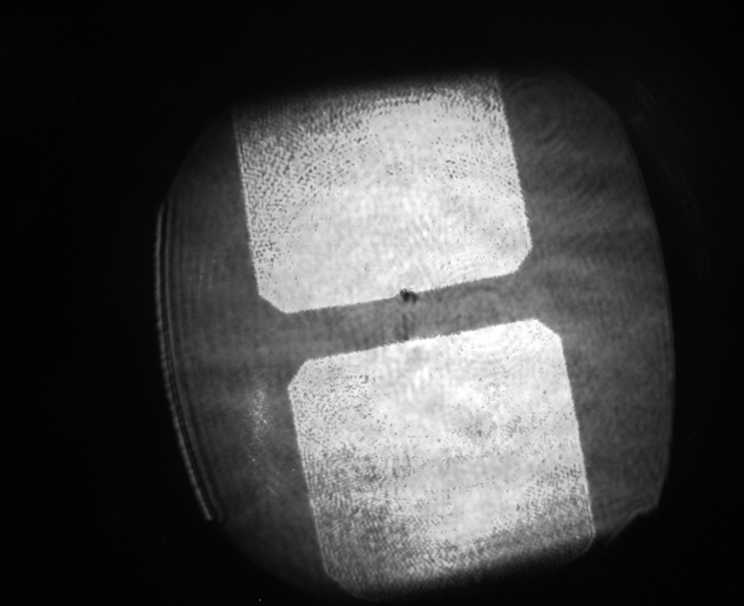
\includegraphics[width=0.5\linewidth]{figures/orion/orion_doublebeamlets_near_field}
	\caption[Image of the ORION SP1 double beamlet structure in the near-field.]{\textbf{Image of the ORION SP1 double beamlet structure in the near-field.} The two beamlets are then superimposed on the target.}
	\label{fig:oriondoublebeamletsnearfield}
\end{figure}

Laser contrast is a major concern for the interaction discussed in this thesis. There is always some spurious signal arriving before the main pulse of interest. In high-power laser systems, this \textit{prepulse} can be itself of ionising intensities, dramatically altering the initial conditions of the system. Generally, the prepulse preheats the plasma leading to expansion. This is catastrophic if one's aim is to interact a laser with a solid density plasma.

The ORION SP2 beamline temporal intensity envelope can be modelled as
\begin{equation}\label{eq:orion_SP2_temporal}
	I_\mathrm{SP2} \sim (I_{0 \ \mathrm{p}}\sech(t/t_\mathrm{p})^2 + I_{0 \ \mathrm{pp}}e^{-(t/t_\mathrm{pp})^2} + I_{0 \ \mathrm{ps}}e^{-\mathrm{abs}(t)/t_\mathrm{ps}} + I_{0 \ \mathrm{ns}}e^{-(t/t_\mathrm{ns})^8}),
\end{equation}
where the constants are detailed in Table \ref{tab:orion_pedestals} \cite{dhillierModelORIONContrast2022}.
\begin{table}[]
	\centering
	\begin{tabular}{lcc}
		\hline\hline
		Pedestal, $i$                & $I_{0 \ i}$ & $t_i$  \\ \hline
		Main pulse, p                & 1           & 0.2 ps \\
		Picosecond pump residual, pp & $10^{-3}$   & 3 ps   \\
		Picosecond pedestal, ps      & \num{5e-5}  & 8 ps   \\
		Nanosecond pedestal, ns      & $10^{-11}$  & 3 ns  \\ \hline \hline
	\end{tabular}
	\caption{\textbf{The native ORION SP2 pulse and prepulse pedestal constants as defined in Equation \ref{eq:orion_SP2_temporal}.}}
	\label{tab:orion_pedestals}
\end{table}
The picosecond pump residual arises from parametric fluorescence in the ps OPA, the picosecond pedestal from scatter in the stretchers and noise on the OPA pump laser and the nanosecond pedestal from parametric fluorescence from the nanosecond OPAs. The `long' duration of the prepulse precludes the use of PIC codes. It is here that the hydrodynamic codes can be more appropriate.
% TODO understand the above, perhaps add more comments
The SP1 temporal intensity profile is
\begin{equation}
	I_\mathrm{SP1} \sim (I_\mathrm{SP2}^2 + I_\mathrm{SP2} \times 10^{-8}).
\end{equation}
The second term arises from limitations in the harmonic separation system. The frequency doubling mechanism is not 100 \% efficient, \textit{i.e.} some of SP2 beamline remains and must be filtered out. The main pulse of the GEMINI beamlines is more appropriately modelled as a Gaussian.
% TODO add a plot of the Gemini contrast
% TODO return to this section once I have read ORION chapter and figured out how I am going to do contrast.


A \ac{PM} is an effective and now standardised tool for the improvement of laser contrast. These single-use optics initially have an \ac{AR} coating of reflectivity $R_1$. As the incident laser fluence passes the damage threshold of the optic, reflecting plasma forms on the front surface. The optic is `switched on' with a reflectivity $R_2$. The \ac{PM} therefore improves the contrast by a factor $R_2/R_1$. There is a balancing act in choosing the peak intensity on the \ac{PM}. Too early and the PM will switch on before the arrival of the main pulse. Too low and there is not enough plasma at the surface at the arrival of the main pulse and $R_2$ is lowered. A peak intensity around \qty{1e16}{W.cm^{-2}} is best \cite{caiTimeresolvedMeasurementsReflectivity2009}. PMs also act as a low-pass spatial filter, improving the quality of the focal spot on target \cite{doumyCompleteCharacterizationPlasma2004}. The use of PMs before the main target ensure the required conditions for a relativistic laser pulse to produce a \ac{RPM}, the main focus of this thesis.

\section{Summary}
This chapter has introduced the field of HED physics. The basic equations that govern the system have been supplied and some simple derivations performed to describe the dynamics of particles in this regime. Details have been given of both suitable simulation codes and laser systems that enable the modelling and generation of the interaction of interest in this thesis. It is now time to present that interaction.
\chapter{\label{ch:2-zvp}The Zero Vector Potential Absorption Mechanism}

\minitoc

\section{Introduction}
Of primary interest in this thesis is the interaction of a relativistically intense short pulse laser interacting with a solid density plasma target with a sharp density gradient. Now is presented the Zero Vector Potential mechanism of attosecond absorption of laser pulse energy, proposed by \textit{Baeva et al} \cite{baevaTheoryHighorderHarmonic2006} and later developed by \textit{Savin et al} \cite{savinAttosecondscaleAbsorptionExtreme2017,savinEnergyAbsorptionLaserQED2019}. Laser energy absorption in dense plasmas was first proposed by Wilks and Kruer \cite{wilksAbsorptionUltraIntenseLaser1992}, a ponderomotive mechanism where plasma electrons are heated directly by the laser pulse via the so-called $\mathbf{J}\times \mathbf{B}$ force.

%At some point I should briefly chat about other absorption models (I think at the end of the intro - this will also include the stuff above. - Then I will start this chapter by talking about the case where JxB does not apply. ALso in the intro specify that for an overdense plasma, the laser does not propagate and must be reflected and hence we are generally talking about a laser-plasma surface interaction and the implications thereof.) Before this point I also want to discuss preplasmas.

This thesis focuses on the so-called `post-ponderomotive' regime where the frequency of the plasma oscillations ($\omega_p \sim \sqrt{n_e}$) are greater than the $\mathbf{J}\times \mathbf{B}$ induced plasma electron oscillations at $2\omega_L$. The plasma electrons are then fast enough to compensate the ponderomotive pressure of the laser pulse with the formation of electrostatic fields between electrons and ions and so respond adiabatically to the $\mathbf{J}\times \mathbf{B}$ force. Hence plasma electrons cannot be heated directly by the laser pulse. Note that this requires a sufficiently steep density gradient around the relativistic critical density surface (where $S=1$) to shift the main interaction to a region where this condition on the overdensity is satisfied. In this case the ponderomotive pressure of the laser compresses the electrons at the front surface of the plasma and so shifts the laser-plasma surface interaction to plasma densities well beyond the relativistic critical density, leaving behind a positive space charge. This electron-ion charge separation leads to the formation of a \textit{pseudo-capacitor} electrostatic field.


Interestingly working through the condition between $\omega_p$ and $\omega_L$ in normalised units suggests the criterion for this regime is $S > 4$, slightly more constraining than $S>1$ as is typically stated \cite{savinModellingLaserPlasmaInteractions2019}.

% at some point I must be explicitely clear about why this conditoin ad my sims with S=1 are compatible. This above criterion on S is associated with the bunch electrons. For S=1 we observe great compression of the target surface enabling us to enter the regime where the bunch S>4 whilst the bulk remains at S=1. Can thsi also be used to explain the energy absorption in phase one (bunch formation) ? Eneryg can be absorbed by JxB until the bunch density goes above some value???



[Come back to this and write up stuff about actaully it being the relativistc frequncy and critical density surfaces that matter and how this does indeed put a stricter condition on the bulk S value]

So we have entered a regime of adiabaticity where the plasma skin layer is confined within a potential well consisting of the ponderomotive pressure and the Coulomb potential. Consider a relativistic linearly polarised laser pulse obliquely incident, with an angle of incidence of $\theta$, on a semi-infinite plasma, existing for $x>0$. The Hamiltonian of a single electron confined within the potential well \cite{goldsteinClassicalMechanics2013} is
\begin{equation}\label{eq:hamiltonian_general}
	\mathcal{H} = c\sqrt{m^2_ec^2 + |\mathbf{p}|^2} - e\Phi.
\end{equation}
Here the first term is the electron energy, $U$, extracted from the invariant of the relativistic 4-momentum of the electron, $\mathbf{P^\mu} = (U/c, \mathbf{p})$,
\begin{equation}
	\mathbf{P^\mu \cdot P_\mu} = \frac{U^2}{c^2} - |\mathbf{p}|^2 = m^2c^2.
\end{equation}
Note that while there has been growing interest in the curvature of spacetime by relativistic lasers [cite edward here], for modern high power lasers this effect is small and not relevant for this thesis. Throughout the inner product of 4-vectors is defined with the Minkowski Metric. [find alex citation on pg 89 of thesis]

The second term of equation \ref{eq:hamiltonian_general} describes the contribution to the electron's energy from the electrostatic potential of the pseudo-capacitor. Decomposing the electron's 3-momentum into orthogonal components: $p_\mathrm{prop}$, along the laser propagation direction, $p_\mathrm{pol}$, along the polarisation axis of the laser pulse and $p_\perp$, perpendicular to both, two simplifications can be made. Firstly, by canonical conservation of transverse momentum, $p_\mathrm{pol} = eA$, where $A$ is the laser vector potential. Secondly, in the case of a $p$-polarised laser pulse (the known optimum for ZVP electron bunch generation), the forces at play confine the electron trajectory to the  $p_\mathrm{prop}$-$p_\mathrm{pol}$ plane and the interaction geometry is in essence \ac{2D}.

[include a diagram alluding to this?-it is basically since B is out of the plane and all other E fields are in the plane, also perhaps provide a foot not here to explain how incidentally this all provides a succinct explanation of why p is better?]

Explicitly, the Hamiltonian is now
\begin{equation}\label{eq:hamiltonian_specific}
	\mathcal{H} = c\sqrt{m^2_ec^2 + p^2_\mathrm{prop} + e^2A^2} - e\Phi.
\end{equation}
From equation \ref{eq:hamiltonian_specific} it is clear that should the vector potential pass through zero, one of the walls of the potential well is suppressed, allowing electrons in the in the skin layer to escape the plasma, breaking adiabaticity. The necessity of vector potential zeros for this violent reconstruction of the plasma surface led Baeva et al \cite{baevaZeroVectorPotential2011} to coin the term `Zero Vector Potential' mechanism to describe this process. Indeed, while in standard calculations a laser pulse will exponentially decay within a skin layer without passing through zero, Baeva et al \cite{baevaZeroVectorPotential2011} were able to demonstrate in \ac{PIC} simulations that for this regime, zeros are able to propagate through the skin layer of the plasma. The explanation for this difference in mechanics relies on a Doppler shift in the laser field due to the relativistic motion of the ablating plasma surface, and the mathematical formalism of this process proceeds as follows.

[I think before this point it would be good to enter in the language of electron bunches or sheaths - I will continue the dicussion assuming this concept has been introduced].

As the \ac{ZVP} mechanism is a relativistic phenomenon, it is essential to consider the laser pulse propagating through a relativistically ablating electron bunch (i.e. with some component of its velocity anti-parallel to the laser pulse propagation direction). Transforming to the rest frame of the ablating front, beyond the relativistic critical density surface, the vector potential of the laser pulse will be an evanescent wave, at the spatial centre of the laser pulse, it can be described simply by
\begin{equation}
	\mathbf{A}'_\mathrm{L}(t',r') = A'_0\cos(\omega'_\mathrm{L}t')\exp(-r'/\delta')\hat{\mathbf{r}}'_\mathrm{pol}= A'_\mathrm{L}\hat{\mathbf{r}}'_\mathrm{pol},
\end{equation}
where the primed symbols indicate that these quantities are measured in the rest frame of the expanding front, $A'_0$ is the vector potential amplitude and $\omega'_\mathrm{L}$ is the frequency of the laser pulse, $r'$ is the propagation distance of the laser into the plasma, $\delta'$ is the skin depth and $\hat{\mathbf{r}}'_\mathrm{pol}$ a unit vector defining the polarisation direction of the laser pulse. Un-primed coordinates will indicate the lab frame measurements.

[For sure include a diagram of this]

While in previous demonstrations of the vector potential zeros, it was assumed that the ablation occurs normal to plasma surface, it is now known that this ablation occurs in the specular reflection direction and it is necessary to confirm that zeros are still predicted. Consider a p-polarised laser pulse confined to the $x$-$y$ plane incident with an angle of incidence $\theta$ on an ablating overdense plasma expanding with velocity $-v_f\hat{\mathbf{x}}$ in the lab frame, as in figure \ref{fig:zvp_ablatingfront}.
% TODO: \usepackage{graphicx} required
\begin{figure}
	\centering
	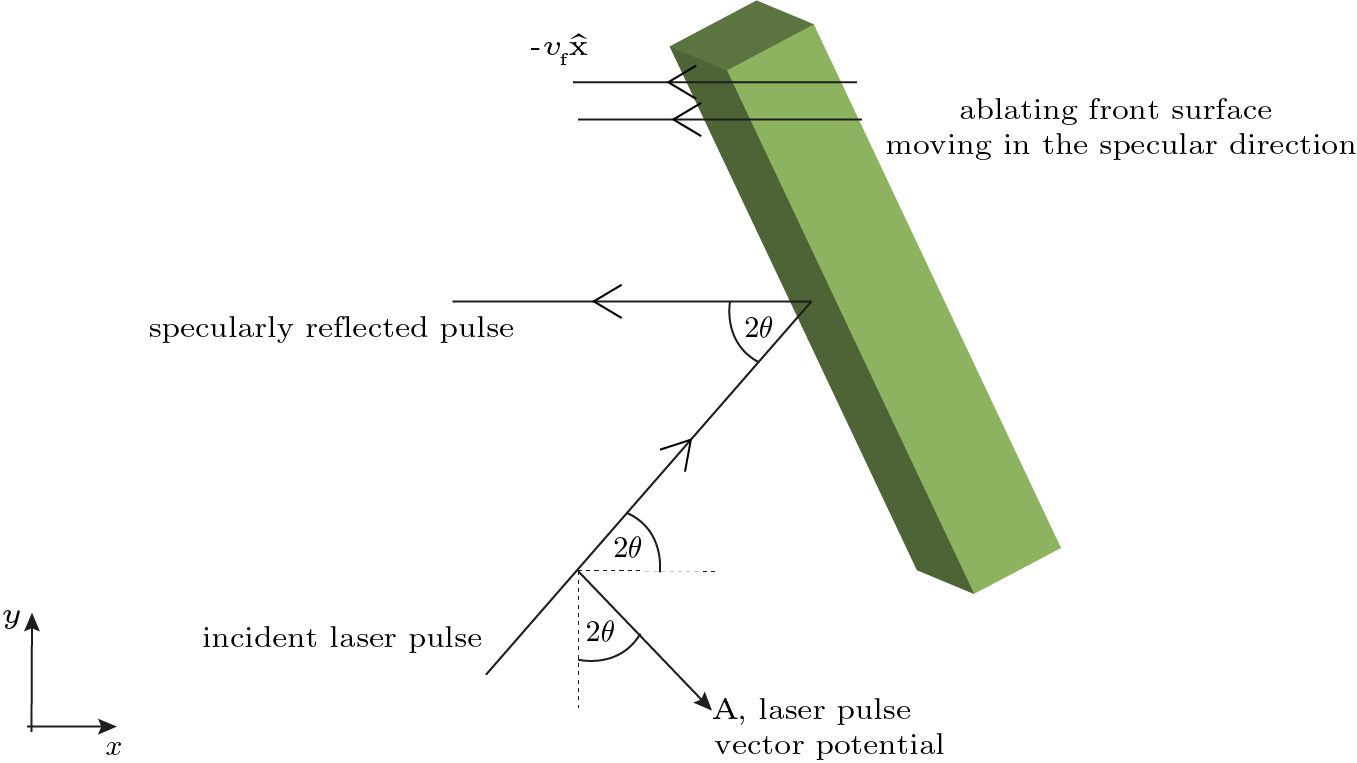
\includegraphics[width=0.7\linewidth]{figures/zvp/zvp_ablating_front}
	\caption{Diagram of a $p$-polarised laser pulse incident on an ablating overdense plasma. The laser is incident obliquely at an angle of $\theta$ and is reflected specularly. The plasma ablates specularly also. The interaction geometry is confined to a 2D plane.}
	\label{fig:zvp_ablatingfront}
\end{figure}
The direction of polarisation is
\begin{equation}
	\hat{\mathbf{r}}_\mathrm{pol} = \hat{\mathbf{x}}\sin{2\theta} - \hat{\mathbf{y}}\cos{2\theta}
\end{equation}
and the velocity of the rest frame of the ablating front relative to the lab frame is $-v_f\hat{\mathbf{x}}$.

Applying the Lorentz transformation to the electromagnetic 4-potential,
\begin{equation}
	\mathbf{A}_\mu = (\phi/c,\mathbf{A}),
\end{equation}
explicitly,
\begin{equation}
	\mathbf{A}'_\mu = \Lambda^\mu_\nu \mathbf{A}_\nu,
\end{equation}
where $\Lambda^\mu_\nu$, the Lorentz transform in this geometry is
\begin{equation}\label{eq:zvp_lorentz}
	\Lambda^\mu_\nu = \begin{pmatrix}
			\gamma & -\beta\gamma & 0 & 0\\
			-\beta\gamma & \gamma & 0 & 0\\
			0 & 0& 1 & 0\\
			0 & 0 & 0 & 1
	\end{pmatrix}
\end{equation}
and here $\beta = -v_\mathrm{f}/c$, $\gamma = 1/\sqrt{1-\beta^2}$. Immediately from the $y$-coordinate transformation,
\begin{equation}\label{eq:zvp_lorentz_y}
	A'_\mathrm{L}\cos{2\theta'} = A_\mathrm{L}\cos{2\theta}.
\end{equation}
Applying the headlight effect for a source moving at an angle $2\theta$ to the boosted frame,
\begin{equation}
	\cos{(2\theta')} = \frac{\cos{(2\theta)}-\beta}{1 - \beta\cos{(2\theta)}}
\end{equation}
and rearranging equation \ref{eq:zvp_lorentz_y}, the vector potential in the lab frame is
\begin{equation}\label{eq:zvp_labA}
	A_\mathrm{L} = \frac{1-\beta \sec{(2\theta)}}{1 - \beta\cos{(2\theta)}} A'_0\cos{(\omega'_L t')}\exp{(-r'/\delta')}.
\end{equation}
Writing the boosted frame space-time coordinates in terms of the lab frame coordinates,
\begin{equation}
	ct' = \gamma(ct-\beta x),
\end{equation}
\begin{equation}
	x' = \gamma(x-\beta ct),
\end{equation}
yields
\begin{equation}\label{eq:zvp_labAfull}
	A_\mathrm{L} =  A_0\cos{(\omega_L t - kx)}\exp{\left(-\frac{\sqrt{(x-\beta ct)^2+(y/\gamma)^2}}{\delta}\right)},
\end{equation}
where
\begin{equation}
	A_0 = \frac{1-\beta \sec{(2\theta)}}{1 - \beta\cos{(2\theta)}}A'_0,
\end{equation}
\begin{equation}
	\omega_L = \gamma \omega'_L,
\end{equation}
\begin{equation}
	k = \frac{\beta \gamma\omega'_L}{c},
\end{equation}
\begin{equation}
	\delta = \frac{\delta'}{\gamma}.
\end{equation}
The oscillatory term in equation \ref{eq:zvp_labAfull} demonstrates the propagation of vector potential zeros within the plasma target. From the structure of this term it would appear that these zeros are expelled from the plasma along the specular direction at a speed (recall beta is negative - change this earlier in the theory so that that negative sign is more explicit in the result.)
\begin{equation}
	v_\phi = \frac{\omega_L}{k} = \frac{c}{\beta} = -\frac{c^2}{v_\mathrm{f}}.
\end{equation}
Could also discuss here about how relativistic similarity theory derives that zeros move at speed c but how that cannot be valid since then we would always have infinitely thin radiation pulses, unless there is an extended range of zero? I suppose there is some radiation happening around the peak? Good questions..
One remaining consideration is we require that the zero gets through the whole electron bunch which is generally at very high density but is also very thin, in a way is this skin depth not what precisely determines the bunch width? The bunch will be compressed until the skin depth goes to zero across it perhaps? Things to think about.


Qualitatively, and in summary, for sufficiently intense laser pulses, electrons on the radiated surface of a solid target are accelerated by the laser to relativistic velocities at a fraction of a laser pulse cycle and therefore electrons both follow similar trajectories and are able to respond adiabatically to the $\mathbf{J}\times \mathbf{B}$ force of the laser pulse. They therefore form a high charge density thin coherent electron sheath on the front surface of the plasma but displaced inwards from the immobile ions (ions are approximately immobile on the timescale of a laser pulse cycle) via the ponderomotive pressure of the laser. This charge separation generates a longitudinal electrostatic pseudocapacitor field that confines electrons to a potential well on the front surface of the plasma, preventing further propagation of the electron bunch into the plasma bulk. When the zero of the vector potential passes through the electron bunch, the ponderomotive pressure instantaneously vanishes and electrons are ejected specularly from the target, copropagating with the zeroes and gaining energy as they discharge the pseudocapacitor field. Coherent sychrotron emission occurs concurrently. The electron bunch is then rotated by the laser pulse and launched into the bulk at high energy.


SOmething to think about: which comes first? electron bunch acceleration across pseudo capacitor or zeros?
Laser accelerates electorns in laser propagation direction , however cannot propagate further into the plasma so only get motion parallel to surface, once potentail well disrupted, accleration is perp to surface so combined, electrons travel in specular direction.
So actually what we are saying is the zeros will go in whatever direction the surface ablates in, but the surface will move in a direction dependent on the components of electron 


\subsubsection{The headlight effect}\label{sec:zvp_headlight}
This most likely goes in the appendix. But storing here for now.

The headlight effect describes the beaming of an isotropically emitting source travelling at some velocity relative to an observer. Consider the geometry of figure \ref{fig:zvp_ablatingfront} with the source (the laser pulse) travelling at an angle $2\theta$ to the observer (in this case, the ablating front). A photon with energy $E$ emitted from the rest frame of the source (in this case the lab frame) has a 4-momentum
\begin{equation}
	\mathbf{P}_\mu = \left(\frac{E}{c},\frac{E}{c}\cos{2\theta},\frac{E}{c}\sin{2\theta}\right).
\end{equation}
As the interaction geometry is confined to a 2D plane,  the $z$-component can be safely neglected. Applying the lorentz boost of equation \ref{eq:zvp_lorentz},
\begin{equation}
	\begin{split}
		\frac{E'}{c} = \gamma \left( \frac{E}{c} - \beta \frac{E}{c}\cos{2\theta}\right) \\
		\frac{E'}{c}\cos{2\theta'} = \gamma \left( \frac{E}{c}\cos{2\theta} - \beta \frac{E}{c}\right).
	\end{split}
\end{equation}
Solving these equations for the angle in the boosted frame,
\begin{equation}
	\cos{2\theta'} = \frac{\cos{2\theta} - \beta}{1-\beta\cos{2\theta}}.
\end{equation}

\subsubsection{Conservation of generalised transverse momentum}\label{sec_app_conservation-generalised-mometum}
This should most likely go in the appendix/ before ZVP Hamiltonian discussion.

Whilst it is commonly stated within the field of laser-solid interactions, it would appear that some nuance/detail is missing from the discussion which in turn shrouds the \ac{ZVP} mechanism in confusion.

Consider a holonomic system of N relativistic particles under the influence of electromagnetic forces. A particle $j$ with charge $e_j$ and mass $m_\mathrm{j}$ experiences a scalar potential,
\begin{equation}
	U_{j} = e_j(\Phi - \mathbf{A} \cdot \mathbf{v}_{j})
\end{equation}
and hence the system is described by the Lagrangian
\begin{equation}
	L = \sum^N_{j=1}\left( - m_\mathrm{j}c^2\sqrt{1-\beta^2_\mathrm{j}} - e_j(\Phi - \mathbf{A} \cdot \mathbf{v}_\mathrm{j}) \right),
\end{equation}
where $\beta^2 = \mathbf{v}_\mathrm{j}\cdot\mathbf{v}_\mathrm{j} /c^2$ \cite{goldsteinClassicalMechanics2013}.
The generalised momentum corresponding to coordinate $x_j$ is
\begin{equation}
	p_{j,x} = \frac{\partial L}{\partial \dot{x}_j} = m_j\dot{x}_j + e_jA_x,
\end{equation}
explicitely, the generalised momentum describes both the linear mechanical momentum and the momentum of the electromagnetic field. Via Noether's theorem, if $L$ is independent of $x_j$, \textit{i.e.} spatially homogeneous along $x$ for particle $j$, then 
\begin{equation}
	\dot{p}_{j,x} = 0.
\end{equation}
Considering a p-polarised Gaussian laser pulse, axis of polarisation along $x$, $A_x$ will be approximately constant. Integrating and noting that initially there is no linear or electromagnetic momentum, the generalised transverse momentum conservation equation for an electron at the plasma-vacuum boundary is obtained, namely,
\begin{equation}
	p_\mathrm{T} = eA,
\end{equation}
where $p_mathrm{T}$ is the electron momentum along the polarisation axis of the laser pulse. and $A$ its vector potential.

Note that this is only valid provided the radiating electron does not radiate along the direction of $\mathbf{A}$ as discussed by Sokolov \textit{et al} \cite{sokolovDynamicsEmittingElectrons2009}. But we do know this radiation is specular so this is true for normal incidence but not specular?? Really need to consider what the EM fields are in the surface from combined Incident and reflected.
The implications of this should maybe be considered?? Also note that this is only true for gaussian pulses with spatial profiles $\gg$ than electron trajectories (\textit{i.e.} twice the relativistic larmor radius).

\subsection{ZVP electron bunch energies}\label{sec:zvp_energies_derivation}
In \cite{baevaZeroVectorPotential2011}, Baeva \textit{et al} propose energy scalings for electron bunches produced in the \ac{ZVP} regime as a function of the laser intensity and plasma density, finding that one of the key statements of similarity theory ($p \sim a_0 S^x$, where $x$ is some integer value, THIS NEEDS A CITE I THINK IT APPEARS IN BAEVAS ORIGINAL HHG PAPER) holds for the \ac{ZVP} mechanism. Later this was then extended to \ac{3D} by Savin \textit{et al} \cite{savinAttosecondscaleAbsorptionExtreme2017}. What follows is that discussion with a more close consideration of the both consequences and constants of proportionality.

(Pherhaps I should redo this discussion condering infinitessimal areas of the plasma surface to show how variation can exist across the surface) Defo do this! And say that provided the variation is small, rel to what though? the surface remains approximately flat -> that is totally not true

Consider again the semi-infinite block of plasma proposed in figure \ref{fig:zvp_ablatingfront}, normally irradiated by a laser pulse with wavelength $\lambda_\mathrm{L}$ and peak electric field, $E_\mathrm{L}$. It is now the ponderomotive pressure of the laser that displaces the electron fluid. Consider ust one laser cycle. The electron surface moves inwards until the pressure exerted by the peak instantaneous ponderomotive pressure of the laser pulse cycle,
\begin{equation}
	\mathbf{P}_\mathrm{L} = \epsilon_0 E^2_\mathrm{L} \hat{\mathbf{x}} = \epsilon_0 \left(\frac{a_0\omega_\mathrm{L}m_\mathrm{e}c}{e}\right)^2 \hat{\mathbf{x}}
\end{equation}
is equal and opposite to the pressure exerted by the pseudo-capacitor field,
\begin{equation}
	\mathbf{P}_\mathrm{C} = \frac{QE}{\sigma} \hat{\mathbf{x}}= -\frac{(en_\mathrm{e}\Delta x)^2}{\epsilon_0}\hat{\mathbf{x}}
\end{equation} 
using equations \ref{eq:intro_Q} and \ref{eq:intro_E}. Equating the magnitudes of $\mathbf{P}_\mathrm{L}$ and $\mathbf{P}_\mathrm{C}$, the maximum displacement inwards of electrons is
\begin{equation}\label{eq:zvp_dx}
	\Delta x \hat{\mathbf{x}} = \frac{c}{\omega_\mathrm{L}}\frac{a_0}{\bar{n}_\mathrm{e}}\hat{\mathbf{x}}  = \frac{1}{kS}\hat{\mathbf{x}},
\end{equation}
where $k$ is the wave-vector of the laser pulse. Correspondingly,
\begin{equation}\label{eq:zvp_E}
	E = \frac{en_\mathrm{e}}{\epsilon_0}\Delta x = \frac{\omega_\mathrm{L}cm_\mathrm{e}a_0}{e} = E_\mathrm{L}.
\end{equation}
Applying the results of equations \ref{eq:zvp_dx} and \ref{eq:zvp_E}, when the ponderomotive pressure vanishes and the electron bunch is launched across the pseudo-capacitor, the relativistic kinetic energy gained by a single electron is
\begin{equation}\label{eq:zvp_T}
	T =  \int \mathbf{F}\cdot\mathrm{d}\mathbf{s} = \int^0_{\Delta x} -eEdx = \int^0_{\Delta x}-\frac{en_\mathrm{e}x}{\epsilon_0}dx = \frac{1}{2}m_\mathrm{e}c^2\frac{a^2_0}{\bar{n}_\mathrm{e}}
\end{equation}
or an electron gamma factor,
\begin{equation}
	\gamma = \frac{1}{\sqrt{1-\beta^2}} = 1 + \frac{a_0^2}{2\bar{n}_\mathrm{e}}.
\end{equation}
Assuming all displaced electrons are captured by the pseudo-capacitor field and launched as a coherent bunch, the total kinetic energy of the electron bunch is
\begin{equation}\label{eq:zvp_U}
	U_\mathrm{ZVP} = n_\mathrm{e}\sigma\Delta x T = \frac{\sigma n_\mathrm{e}}{k}\times m_\mathrm{e}c^2 \frac{a^3_0}{\bar{n}_\mathrm{e}}.
\end{equation}
It is now interesting to compare equation \ref{eq:zvp_U} to the laser energy deposited upon the plasma surface and therefore consider what fraction of the laser energy can be absorbed via the \ac{ZVP} mechanism. Using $E = E_\mathrm{L}$, \ref{eq:zvp_U} can be rewritten as
\begin{equation}
	U_\mathrm{ZVP} = \frac{1}{2\omega_\mathrm{L} S}\sigma c \epsilon_0 E^2_\mathrm{L}.
\end{equation}
For the case of normal incidence, bunches are produced at a frequency of $2\omega_\mathrm{L}$, naturally following the frequncy of the $\mathbf{J}\times \mathbf{B}$ force. Assuming a sinusoidal plane wave incident with surface area $\sigma$, the energy absorbed in half a laser cycle is
\begin{equation}
	 U_\mathrm{L,1/2} = \sigma \frac{T}{2}\langle I_\mathrm{L}\rangle = \frac{2\pi}{4\omega_\mathrm{L}}\sigma c\epsilon_0E^2_\mathrm{L}.
\end{equation}
Hence,
\begin{equation}
	\eta_\mathrm{ZVP} = \frac{U_\mathrm{ZVP}}{U_\mathrm{L,1/2}} = \frac{1}{\pi S}.
\end{equation}
Interestingly, this new analytical result predicts the trend observed by A. Savin \cite{savinModellingLaserPlasmaInteractions2019} in \ac{PIC} simulations both in magnitude and in scaling. Indeed, A. Savin demonstrated 
\begin{equation}
	\eta_\mathrm{ZVP} \sim S^{-1.000(3)},
\end{equation}
however, this result led A. Savin to conclude increasing $S$ increases the energy in the reflected \ac{HHG} beam thus increasing high harmonic efficiency, seemingly in tension with the vast majority of the work on this regime [CITE CITE CITE]. The resolution arises from the follwoing: there are two distinct conversion efficiencies which describe the reflected harmonic spectrum: the conversion efficiency into the whole reflected beam and the conversion efficiency into individual harmonics. While the total conversion into the reflected beam decreases for decreasing $S$, the slope of the harmonic spectrum also decreases and therefore while A. Savin is absolutely correct, the imporant parameter (the slope of the harmonic spectra) follows the opposite trend.

Indeed high X-ray harmonic efficiency neccesitates high inefficiencies in the production of ZVP electron bunches as higher energy bunches produce more coherent reflected radiation, a caveat not often considered in the quest for higher-order harmonics.


[Side note for my reference: bunch is made and at peak compression at peak of laser pulse. then laser field oscillates,inside the bunch they experience an a0 = 0(? maybe) outside there is a minimum in the field, then the bunch is rotated back when it hits the next peak of the laser pulse (ie a0=0? outside plasma?) the upshot of this is I can then say there is a distance of lambda/2 between bunch peak displacement and radiation point and since peak displacement = 1/kS, for all S, the pseudocapacitor has been completely discharged and therefore there has been the maximum energy gain before HHG production - important for electron bunch gamma factor discusion.]


Next up: the unification of RES and ZVP.

\subsection{ZVP bunches oblique incidence scaling and internal bunch structure}
This section is inspired by \cite{gonoskovUltrarelativisticNanoplasmonicsRoute2011} and \cite{vincentiOpticalPropertiesRelativistic2014} supplementary material but different where I believe they have gone wrong to generalise the \ac{ZVP} mechanism energy scalings.

The below section needs cleaning up of minus signs etc, take the convention laser propagates in the positive direction therefore drift of electrons and ions in frame with normal incidence is in negative direction.

As has previously been stated, if the plasma-vacuum boundary is sufficiently steep, the plasma electrons will respond adiabatically to the laser pulse and arrange themselves to form a pseudocapacitor longitudinal electric field $E_\mathrm{C}$ at the plasma surface. At all points in this adiabatic phase, the surface electrons will be in a quasi-static equilibrium \textit{i.e.} there will be a balance between the electromagnetic forces on them. Consider again a laser pulse incident on a solid density plasma existing for $x>0$ at angle $\theta$. Transforming to the reference frame where the laser is incident normally (quantities in this frame are indicated by the primed symbol), the electron and ion bulk plasma species are now streaming with a velocity $\mathbf{v}_\mathrm{d} = -c \sin\theta \hat{\mathbf{y}}$.  From the Lorentz force law along the longitudinal direction ($\hat{\mathbf{x}}$), for a displacement of the electron fluid $x'_\mathrm{e}$ (one assumes that the expression for a single electron at the surface describes the surface as via relativity all electrons follow similar trajectories), travelling at speed $\mathbf{v'}$
\begin{equation}\label{eq:zvp_eq}
	-e(\mathbf{v'}(x'_\mathrm{e})\times (\mathbf{B}'_\mathrm{L}(x'_\mathrm{e}) + \mathbf{B}'_\mathrm{i}(x'_\mathrm{e}))\cdot \hat{\mathbf{x}} + E'_\mathrm{C}(x'_\mathrm{e}) )= 0,
\end{equation}
where 
\begin{equation}\label{eq:zvp_Bl}
	B'_\mathrm{L} = \frac{m_\mathrm{e} \omega'_\mathrm{L}a_0\sin(\omega'_\mathrm{L}t'-k'x'_\mathrm{e})}{e} \hat{\mathbf{z}}
\end{equation}
and $B_\mathrm{i}$ originates from the uncompensated ion current, $\mathbf{J_\mathrm{i}} =  Zen'_\mathrm{i}(x'_\mathrm{e}) \mathbf{v}_\mathrm{d}$, where the electron fluid has been displaced. As before, from equation \ref{eq:intro_E},
\begin{equation}\label{eq:zvp_Ec}
	E'_\mathrm{C} = \frac{en'_\mathrm{e}x'_\mathrm{e}}{\epsilon_0}.
\end{equation}
Note that there is no contribution to the laser magnetic field here from the reflected laser pulse since the assumption is that during this pushing phase all laser pulse energy is converted into electrostatic potential energy, this is supported by the attosecond duration of the reflected harmonic beam (\textit{i.e.} it is not produced during this phase). Maxwell-Ampère's Law states
\begin{equation}\label{eq:zvp_maxwellampere}
	\nabla \times \mathbf{B} = \mu_0 \mathbf{J}.
\end{equation}
Noting that by symmetry there can be no variation in the magnetic field with $y'$ or $z'$ it becomes clear that
\begin{equation}\label{eq:zvp_BiJi}
	-\frac{\mathrm{d}(\mathbf{B}'_\mathrm{i})_{z'}}{\mathrm{d} x'} = \mu_0 (\mathbf{J}_\mathrm{i})_{y'}.
\end{equation}
Integrating equation \ref{eq:zvp_BiJi} from $-\infty$ to $x'_\mathrm{e}$, noting that $\mathbf{B}_\mathrm{i} = 0$ at infinity and assuming a constant density profile $n'_\mathrm{i}$ for $x>0$,
\begin{equation}\label{eq:zvp_Bi}
	\mathbf{B}'_\mathrm{i}(x'_\mathrm{e}) = \mu_0 en'_\mathrm{e}x'_\mathrm{e}c\sin(\theta)\hat{\mathbf{z}}.
\end{equation}
Using equations \ref{eq:zvp_Bl}, \ref{eq:zvp_Ec} and \ref{eq:zvp_Bi} and making the very reasonable approximation that the relativistic electrons on the surface move at speed $v'_y \approx \pm c$ at peak displacement ($x'_\mathrm{e} = x'_\mathrm{p}$), \ref{eq:zvp_eq} can be written as
\begin{equation}
	-e\left(\pm c\left(\pm\frac{m_\mathrm{e}\omega'_\mathrm{L}a_0}{e} + \mu_0 en'_\mathrm{e} x'_\mathrm{p}c\sin\theta\right)+\frac{en'_\mathrm{e}x'_\mathrm{p}}{\epsilon_0}\right) = 0.
\end{equation}
Note that to be in the laser pushing phase the first term must be negative, corresponding to $\mathbf{v'}$ and $\mathbf{B}'_\mathrm{L}$ having the opposite sign, hence,
\begin{equation}
	 c\left(-\frac{m_\mathrm{e}\omega'_\mathrm{L}a_0}{e} \pm \mu_0 en'_\mathrm{e} x'_\mathrm{p}c\sin\theta\right)+\frac{en'_\mathrm{e}x'_\mathrm{p}}{\epsilon_0} = 0,
\end{equation}
where here the $\pm$ tracks the sign of $\mathbf{v}'$. After some maniputation, one arrives at
\begin{equation}
	x'_\mathrm{p} = \frac{1}{k'S' (1\pm \sin\theta)}.
\end{equation}
Transforming back to the lab frame, naturally,
\begin{equation}
	x_\mathrm{p} = \frac{1}{kS(1\pm \sin\theta)}.
\end{equation}
Already this is quite a result, reducing to equation \ref{eq:zvp_dx} for $\theta =0$ and predicting the suppression and enhancement of the two surface oscillations per laser puse cycle. Explicitely, for a laser pulse propagating at $y = x\tan\theta$, the peak displacement of the electron surface is enhanced for $\mathbf{B}_\mathrm{L}$ in the $+\hat{\mathbf{z}}$-direction and suppressed for $\mathbf{B}_\mathrm{L}$ in the $-\hat{\mathbf{z}}$-direction.

Consider now acceleration of the electron bunch across the pseudocapacitor field in the boosted frame,
\begin{equation}\label{eq:zvp_Tp}
	T' = \int \mathbf{F}'\cdot \mathrm{d} \mathbf{s}' = \int^0_{x'_\mathrm{p}} -eE'_\mathrm{C}(x'_\mathrm{e}) \mathrm{d}x'_\mathrm{e} =  \frac{en'_\mathrm{e}(x'_\mathrm{p})^2}{2\epsilon_0}=\frac{1}{2}m_\mathrm{e}c^2\frac{a^2_0}{\bar{n}'_\mathrm{e}(1\pm \sin\theta)^2}.
\end{equation}
Again, transforming back to the lab frame, noting the gain in energy from crossing the pseudo-capacitor 


The linearity of four-vectors ensures 
\begin{equation}
	\mathbf{\Delta P}^\mathrm{\mu} = (\frac{\Delta E}{c}, \mathbf{\Delta p})
\end{equation}
is also a four-vector. The Lorentz transform for change in energy is thus
\begin{equation}
	\Delta E = \gamma \left(\Delta E' - \frac{\mathbf{v}_\mathrm{d}}{c}\cdot \mathbf{\Delta p'}\right),
\end{equation}
where 
\begin{equation}\label{eq:zvp_gamma}
	\gamma = \frac{1}{\sqrt{1+\sin^2\theta}} = \frac{1}{\cos\theta}.
\end{equation}
Hence for energy gain $\Delta E' = T'$ in the boosted frame (where $\Delta p_y = 0$),
\begin{equation}
	T = \gamma T'.
\end{equation}
Using equations \ref{eq:zvp_Tp} and \ref{eq:zvp_gamma} and recalling $\bar{n}_\mathrm{e} = \bar{n}'_\mathrm{e}/\gamma$,
\begin{equation}\label{eq:zvp_Tzvp_theta}
	T =m_\mathrm{e}c^2 \frac{a_0}{2S(1\pm\sin\theta)^2}
\end{equation}
Nb this could have simply been established in the lab frame and considering F.ds which is just the same[The electron bunch then accelerates across the pseudo-capacitor in the specular direction, the force ] maybe put this derivation in appendix.

Also note that when doing this transformation, T is the energy gained but there is another term in the momentum from the transform, since now $v_y = c\sin\theta$. This is unrelated to the energy gain from crossing the pseudo capacitor. There is no explanation of where this energy comes from, just that in order for the bunch to travel in the -x direction in the boosted frame - not sure what real explanation there is for this to occur, also confusion here since is this actually contained within the gamma expression or not, im lost come back to this. Maybe actualyl this is fine. We jsut take the gamma factor associated with the py gain ($=\sec\theta$ - corresponding to a gamma of 1.4 at 45 degrees) and add the delta gamma from the pseudo capacitor and that should be fine.

Another note: this dependence on theta ($1\pm \sin\theta$) can be explained as an increase due to the electric field having a component acting either in or out from the plasma surface either assisting or counteracting the magnetic field.

Idea: Can one use an external constant magnetic field to obtain the same results for normal incidence?

Also need to go back through this section and make clear which gamma is which in this section

Therefore, as with peak displacement, the energy gained by the electron bunch via the ZVP mechanism is suppressed in one half cycle and enhanced in the second.

While this model would suggest an optimal angle for electron energy and therefore \ac{HHG} of $\pi/2$, if $\theta > \pi/4$, then, if the relativistic electron bunch is travelling at $c$ along the specular reflection direction, the subsequent laser peak amplitude will never `catch up' with the electron bunch, and electrons will escape through the antinodes (?) of the electric field [CITE KRUSHELNICK PAPER GRAZING INCIDENCE ELECTRONS], generating high charge electron bunches in reflection, but decreasing \ac{HHG efficiency}.

Finally, moving on to the calculation of total bunch energy as a function of $\theta$. Since the total number of electrons in the accelerating bunch must be invariant,
\begin{equation}\label{eq:zvp_Uzvp_theta}
	U_\mathrm{ZVP}(\theta) = n_\mathrm{e}\sigma\Delta x T(\theta) =  \frac{\sigma n_\mathrm{e}}{k}\times m_\mathrm{e}c^2\frac{a_0}{2S^2(1\pm \sin\theta)^3}.
\end{equation}
What we can see from this is this enables a larger fraction of the laser energy to be absorbed at high $S$ pushing the currently experimentally accessible regime into the most efficient regime.

I want to move on, but return to this section and sort out the following. 


Another concern: peter showed me sims that suggested that increasing S incerased the suppressed oscillations more RELATIVE to the main oscilisations, perhaps need to look at the internal bunch structure?

Also see if can do a second order calculation through the electron bunch to see if can calculate its structure.



Big note:
The highest electron gamma factors comes from those electrons at the very front surface who are accelerated before high density is reached and quasistatic equilibrium reached (there are therefore very few of them), these few electrons do not satisfy ZVP relation for energy, instead 
ponderomotvie + ZVP which at most would be twice the predicted gamma which is quite some difference HOWEVER for all experiments so far, ZVP energy gain is small since S large so ponderomotive is more sensible.



Earlier write something along the lines of explaining while ZVP absorption does represent laser energy absorption, bulk heating occurs rather indirectly.

\section{Defining characteristics of the ZVP mechanism}
In her original paper, T. Baeva \textit{et al} \cite{baevaZeroVectorPotential2011} outlined 6 defining characteristics of the \ac{ZVP} mechanism, namely,
\begin{enumerate}
	\item The existance of vector potential zeros moving through the skin layer in the laboratory frame;
	\item The existance of zeroes in the incident laser pulse vector potential required for the formation of fast electron bunches;
	\item The generation of fast electron bunches with ultra-short temporal duration;
	\item Such bunches should be described by the expressions for average \ref{eq:zvp_Tzvp_theta} and total energy \ref{eq:zvp_Uzvp_theta};
	\item An intrinsic link must exist between the fast electron bunches and coherent X-ray \ac{HHG};
	\item Injection of the fast electron bunches along the propagation axis of the laser pulse;
\end{enumerate}
with the essential point being it is the moving zeros within the skin layer being the defining delineator between this post-ponderomotive regime of laser pulse energy absorption and all other proposed mechanisms. While such observational requirements are far beyond the reaches of currently experimental know-how, numerical simulations in both 1- \cite{baevaZeroVectorPotential2011} and 2-dimensions \cite{savinAttosecondscaleAbsorptionExtreme2017} have confirmed the above points. Now is presented the first \ac{3D} simulations to demonstrate the \ac{ZVP} mechanism.

\section{Numerical simulations of the ZVP mechanism}
This thesis relies throughout on the analysis of 1,2 and 3D \ac{PIC} simulations, primarily using the massively-parallel and open-source simulation code Smilei \cite{derouillatSmileiCollaborativeOpensource2018}. Simulation parameters will be provided throughout.
\subsection{The ZVP mechanism in 3D}
Results are presented in figure \ref{fig:zvp3d}.
% TODO: \usepackage{graphicx} required
\begin{figure}
	\centering
	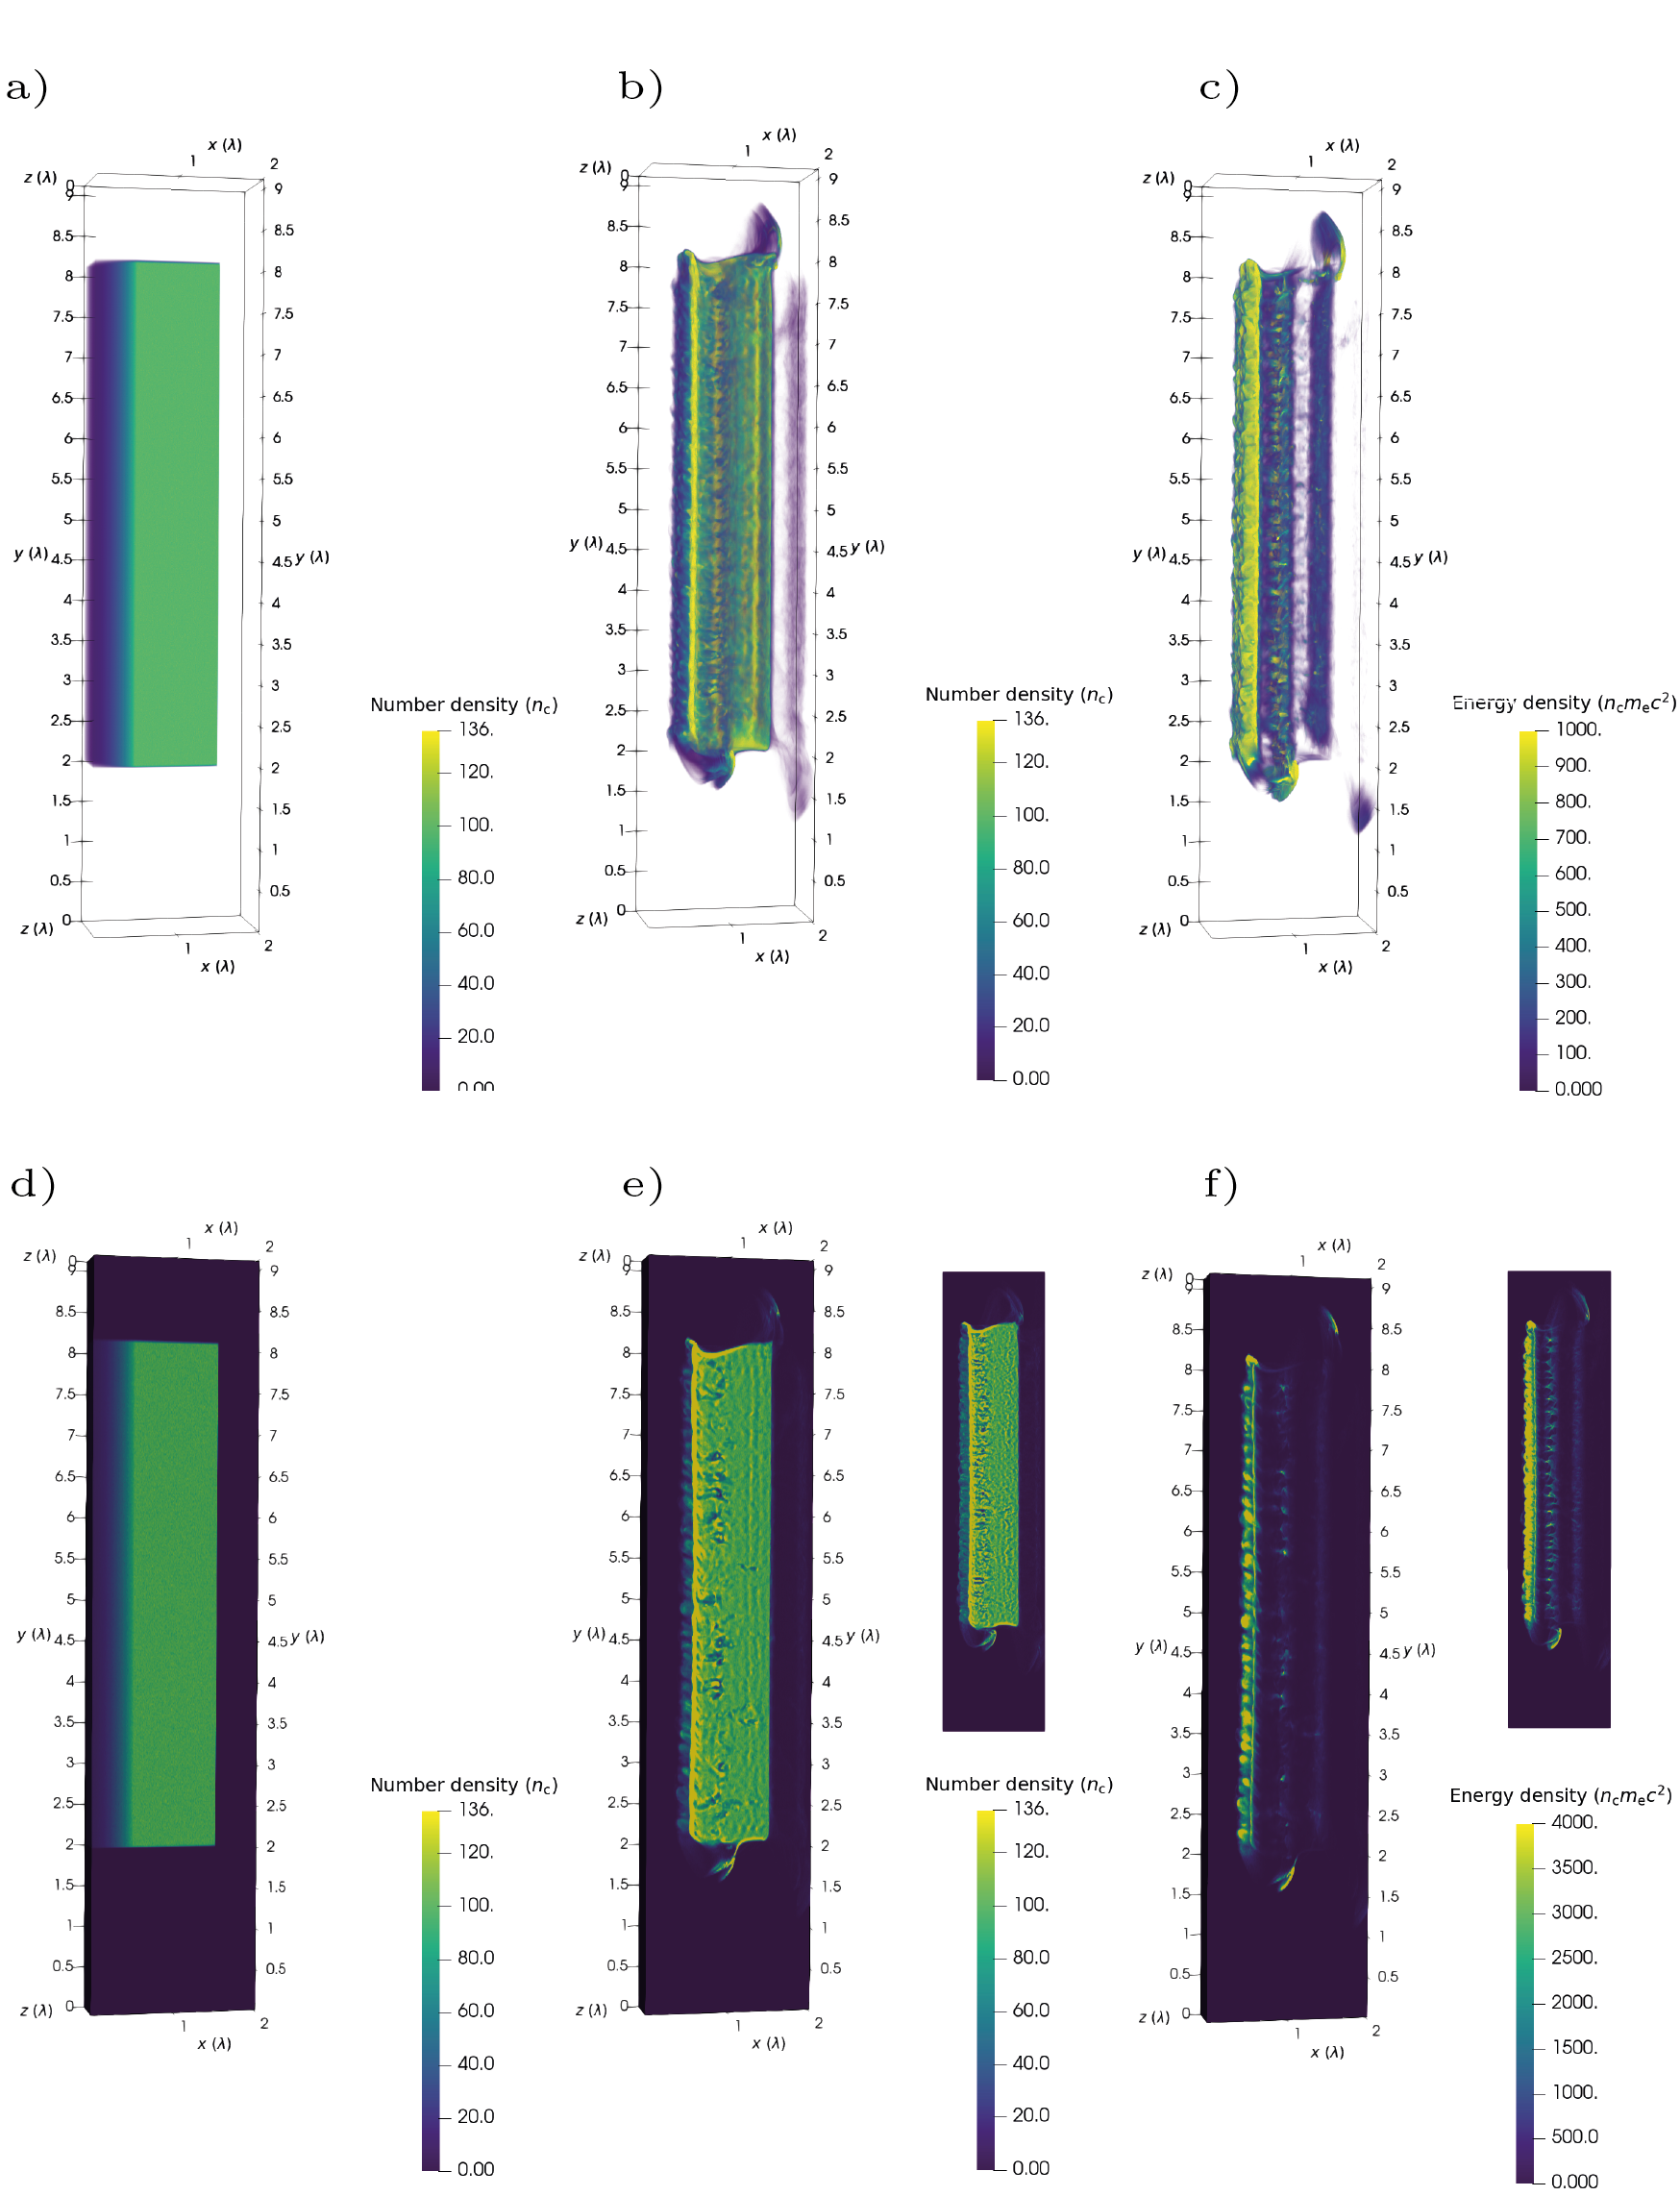
\includegraphics[width=1\linewidth]{../figures/zvp_3D}
	\caption{Simulation results from a 3D \ac{PIC} simulation of the \ac{ZVP} mechanism. a) The initialised electron number density. b) The electron number density several cycles later, the plasma bulk is intact, however there is evidence of instabilities and electron bunches propagating through and around the plasma. c) The electron kinetic energy density at the same timestep. Note that the scale has been clipped to enable observation of both electron bunches propagating through and around the plasma bulk. Significantly higher energy density, corresponding to a higher charge density and attosecond duration for the electron bunches propagating around the bulk. d-f) Plots clipped through $z=0$ for a-c) respectively for better clarity on the internal structure of the plasma bulk.}
	\label{fig:zvp3d}
\end{figure}


Note that the bounds for the plots of KE dens have been chosen to enable observation of both hot electron bunches through centre and around sides (those to the sides have dramatically higher energy densities - related in part due to the maintenance of the as duraction.)

Interesting result of the 3D sim: Can see bunch on front surface and laser clearly propagating behind it. Is this since in this new regime (ZVP dominating HHG) the thin bunch barely attenuates (ie reflects) the laser pulse when it is accelerating across the pseudo capacitor, hence the laser is still effectively able to compress the plasma surface and keep the process going. Meanwhile the reflected HHG light comes mostly from converting bunch KE into HHG.

\subsection{Typical ZVP electron bunch properties}
Then section of a typical bunch properties 
While much has been stated of the high energy and short duration of ZVP bunches in the previous work, the specific properties of such bunches has largely avoided interrogation.

\subsection{Parameter scan of electron bunch mean energy}

\subsection{Total electron bunch energy scaling}


Then Energy scalings

Then QED?
Then experiment?




\chapter{\label{ch:x-misc}Miscellaneous notes}

\minitoc

\section{To do}

\begin{enumerate}
	\item HYADES simulations
	\item Add more citations
	\item Similarity theory details in appendix
	\item Add details on CPA and OPCPA
	\item Simulation algorithms (details in appendix?)
	\item Velocity transformations derivation (appendix)
	\item Sources of error system
	\item Ponderomotive heating mechanisms
	\item Fix QED section
	\item Particle merging
	\item Radiating particles and relativistic larmor radius
	\item smieli performance plot
	\item A collisionless fully ionised plasma
	\item Basic derivation of the Schwinger limit
	\item Calculating collision frequency
	\item Feynmann diagrams
	\item Add some detail of vectorisation
\end{enumerate}

On the ZVP front
\begin{enumerate}
	\item Fix diagrams
	\item Go through discussions
	\item Add errrors plot
	\item Check out new sims
	\item Conclusion
	\item Shape of transverse momentum (more parabolic compared to linear and explanaition of bunch holding together), Shrp front edge then parabolic (or even exponential decay - it is defo expoenential)
	\item a0 convention, when max and when varying in time
	\item Editing
\end{enumerate}

\section{ORION experiment} 
The following derivation determines the polarisation of the ORION laser pulses in the experiment and the boostes frame quantities for the PIC simulations.

I will have a whole subsection devoted to the different frames of reference of relevance and then a second one about normalised units. What follows now is the derivation of the boosted frame in which the laser is incident normally relative to the lab frame where the laser is incident obliquely.

I will try to use a consistent convention for coordinate system as much as possible.

\subsection{Frames of reference}
Other frames of reference include, HB front surface at rest frame, ablating front frame, smilei frames. 

When writing out the pistoning equation in full in thesis, include analysis in Robinson 2009 to do it for multiple ion species.



I should go over this and use third year relativity notes to formalised and make more consistent.

While some of this section may seem trivial, it is frequently miscalculated in the literature, it therefore seems of great importance to provide a full derivation.

The following is inspired by \cite{bourdierObliqueIncidenceStrong1983}, here they give the formula for k and omega.

In \cite{bourdierDynamicsChargedParticle2001} they determine the normalised vector potential, if defined similarly in the new frame, then it is frame invariant. This fails to consider what about the fact that the vector potential is in reality more complex and is not simply the temporal integral of the electric field. Nonetheless it is still reasonable to define it so if what is of real importance (as is usually important) is in fact the fields and it is simply being used as a way to normalise the field intensity.

Consider a photon incident on a plasma block at angle $\theta$ as in figure \ref{fig:miscreferenceframesboosted1d}.
% TODO: \usepackage{graphicx} required
\begin{figure}
	\centering
	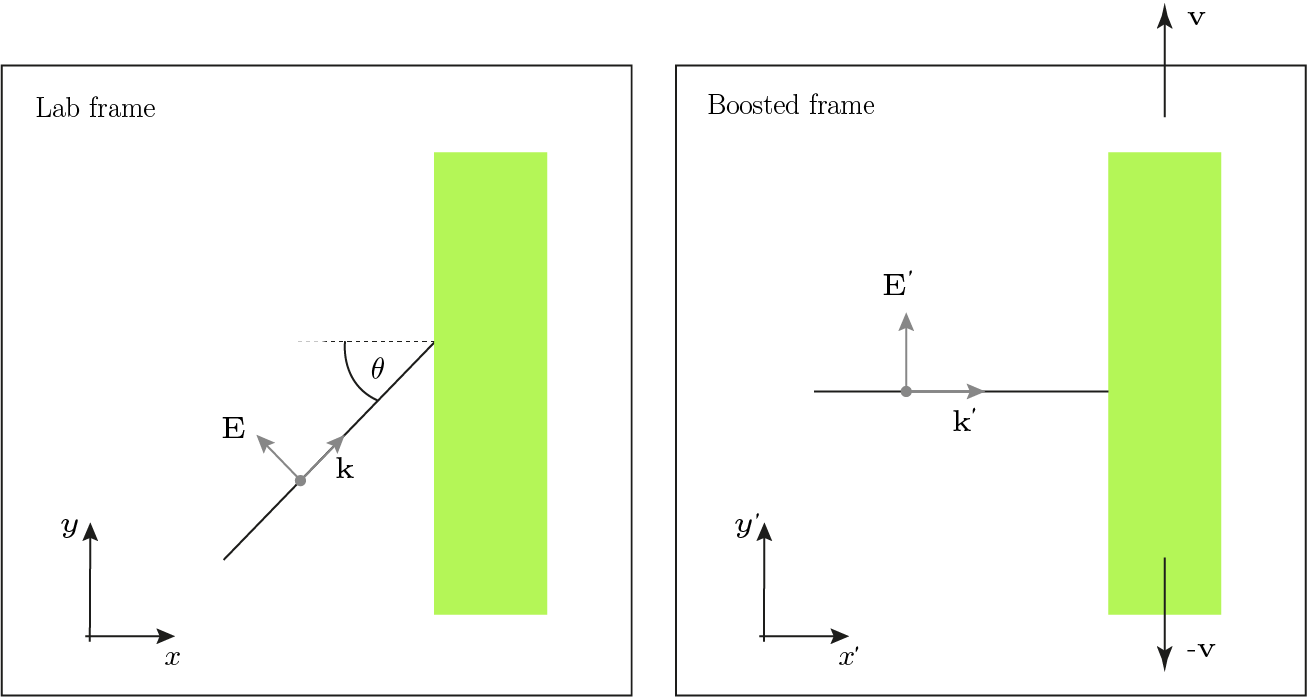
\includegraphics[width=1\linewidth]{figures/misc/misc_reference_frames_boosted_1D}
	\caption{}
	\label{fig:miscreferenceframesboosted1d}
\end{figure}
A boost is applied with velocity $\mathbf{v}$ to a frame such that the photon is normally incident on the now streaming plasma at velocity $-\mathbf{v}$. The velocity transformation for the photon's velocity, $\mathbf{u}$, parallel to the boost is
\begin{equation}
	\mathbf{u}'_\parallel = \frac{\mathbf{u}_\parallel - \mathbf{v}}{1-\mathbf{u}\cdot\mathbf{v}/c^2}.
\end{equation}
Setting  $\mathbf{u}'_\parallel = 0$, it is clear that
\begin{equation}
	\mathbf{v} = \mathbf{u}_\parallel = c\sin\theta \hat{\mathbf{y}}
\end{equation}
in this geometry and 
\begin{equation}
	\gamma_\mathbf{v} = \frac{1}{\sqrt{1-\mathbf{v}^2/c^2}}=\sec\theta.
\end{equation}
Noting that since Snell's law is frame invariant, the photon remains normal as it propagates into the skin depth of the plasma, a frame in which the interaction reduces to a 1D problem has been successfully found for all $\theta < \pi/2$. Those familiar with the topic may wonder how this is possible considering the `ripples' that are observed on the plasma surface for oblique incidence. The explanation for this is of course the relativity of simultaneity. It remains to determine how do all the relevant quantities transform as such a boost is applied. Starting with an easy one: the photon's wave four-vector is 
\begin{equation}
	\mathbf{K}^\mathrm{\mu} = \left(\frac{\omega}{c},\mathbf{k}\right)
\end{equation}
and thus the freqency transforms as
\begin{equation}
	\frac{\omega}{c} = \gamma_\mathbf{v}\left(\frac{\omega'}{c}-\frac{\mathbf{v}}{c}\cdot\mathbf{k'}\right).
\end{equation}
Since $\mathbf{v}\cdot\mathbf{k'} = 0$, 
\begin{equation}\label{eq:boost_omega}
	\omega' = \omega\cos\theta .
\end{equation}
As 
\begin{equation}
	n'_\mathrm{c} = \frac{m_\mathrm{e}(\omega')^2}{4\pi e^2},
\end{equation}
\begin{equation}\label{eq:boost_nc}
	n'_\mathrm{c} =n_\mathrm{c} \cos^2\theta ,
\end{equation}
while the plasma block will be Lorentz contracted along $\hat{\mathbf{y}}$, hence the number density of electrons will increase as,
\begin{equation}
	n'_\mathrm{e} = \frac{n'_\mathrm{e}}{\cos\theta},
\end{equation}
leading to the perhaps unexpected
\begin{equation}
	\bar{n}'_\mathrm{e} = \frac{\bar{n}_\mathrm{e}}{\cos^3\theta}.
\end{equation}
Time is dilated 
\begin{equation}
	t' = \frac{t}{\cos\theta}.
\end{equation}

Consider now the more general case (I should jsut simply replace my diagram with a 3D one that incorporates this initially) where the photon's electric field is rotated out of the $x$-$y$ plane, \textit{i.e.}
\begin{equation}
	\mathbf{E} = E_0(-\cos\phi\sin\theta,\cos\phi\cos\theta,\sin\phi)
\end{equation}
and correspondingly
\begin{equation}
	\mathbf{B} = \frac{\hat{\mathbf{k}} \times \mathbf{E}}{c}= \frac{E_0}{c}(\sin\phi\sin\theta,-\sin\phi\cos\theta,\cos\phi).
\end{equation}
The Lorentz transformations for electro-magnetic fields are
\begin{equation}
	\mathbf{E}'_\parallel = \mathbf{E}_\parallel,
\end{equation}
\begin{equation}
	\mathbf{B}'_\parallel = \mathbf{B}_\parallel,
\end{equation}
\begin{equation}
	\mathbf{E}'_\perp = \gamma_\mathbf{v}(\mathbf{E}_\perp + \mathbf{v} \times \mathbf{B}),
\end{equation}
\begin{equation}
	\mathbf{B}'_\perp = \gamma_\mathbf{v}(\mathbf{B}_\perp - \mathbf{v} \times \mathbf{E}/c^2).
\end{equation}
Using the above expressions for $\mathbf{E}_\perp$ and $\mathbf{E}_\parallel$ and transforming to the boosted frame,
\begin{equation}
	\mathbf{E}' = E_0\cos\theta (0,\cos\phi,\sin\phi).
\end{equation}
As anticipated for normal incidence there is no component of the E-field normal to the surface. Conveniently, the polarisation of the incident photon is unchanged despite having components both parallel and perpendicular to the transformation and 
\begin{equation}
	|\mathbf{E}'| = |\mathbf{E}|\cos\theta.
\end{equation}
The picture can now be completed. Since
\begin{equation}
	a_0' = \frac{e|\mathbf{E}'|}{m_\mathrm{e}e\omega'}
\end{equation}
it follows that
\begin{equation}
	a_0' = a_0,
\end{equation}
\begin{equation}
	S' = \frac{S}{\cos^3\theta}.
\end{equation}


\subsubsection{Four-potential transformation}
Consider a laser pulse obliquely incident, angle $\theta$, it has 4-vector potential $\mathbf{A}^\mu = (0, A\sin\theta,A\cos\theta,0)$, where $A = A_0\sin(\mathbf{k}\cdot\mathbf{x} - \omega t)$ and $\mathbf{k} = (k\cos\theta,k\sin\theta,0)$. Applying the lorentz transformation, in the frame where the laser pulse is normally incident,
\begin{equation}
	\mathbf{A}'^\mu = (-\gamma\beta A\cos\theta/c,  - A\sin\theta, \gamma A\cos\theta,0) = (-A\sin\theta, -A\sin\theta, A,0) 
\end{equation}
since $\beta = \sin\theta$ in the positive $y$ direction and $\gamma = 1/\cos\theta$.

Therefore,
\begin{equation}
	\mathbf{E}'/\cos(\mathbf{k}\cdot\mathbf{x} - \omega t) = --\sin\theta\cos\theta k A_0\hat{\mathbf{x}} --- \sin\theta\cos\theta \omega A_0\hat{\mathbf{x}} + A_0\omega\cos\theta = A_0\omega',
\end{equation}
since $\sin(\mathbf{k}\cdot\mathbf{x} - \omega t) = \sin(x'k\cos\theta-\omega t'\cos\theta)$
Note I have been sloppy here with factors of $c$.

Do it does look at though the vector potential amplitude is unchanged by the transformation but it is more subtle, it is useful to define an $a_0' = eE/m_\mathrm{e}\omega$ to normalise the electric field intensity but note that this cannot be converted into the actual vector potential, it is just a useful construct.

Also note that whatever the transverse vector potential is in the boosted normal incidence frame is simply whatever the amplitude of the vector potential is in the oblique incidence frame.

\subsection{ORION interaction geometry}
The ORION target chamber has its own defined geometry with the target located at the origin, described in figure \ref{fig:miscoriontargetchambergeometry}.
% TODO: \usepackage{graphicx} required
\begin{figure}
	\centering
	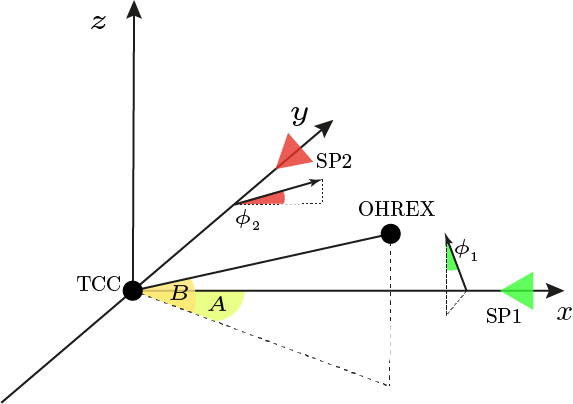
\includegraphics[width=0.5\linewidth]{figures/misc/misc_ORION_target_chamber_geometry}
	\caption{ORION target chamber geometry showing the location of the target (TCC) and OHREX spectrometer and the green (SP1) and infra-red (SP2) beamlines and their corresponding polarisations.}
	\label{fig:miscoriontargetchambergeometry}
\end{figure}
The polarisation angles are $\phi_1 = \qty{11.8}{\degree}$ and $\phi_2 = \qty{16.4}{\degree}$. Following reflection of the infra-red beam off the plasma mirror, both the green and infra-red lasers propagate in the -$\hat{\mathbf{x}}$-direction  towards the origin. The OHREX crystal is located at 
\begin{equation}
	\mathbf{r}_\mathrm{OHREX} = r_0(\cos B\cos A,-\cos B\sin A, \sin B),
\end{equation}
where $r_0 = \qty{2.4}{m}$, $A = \qty{26.82} {\degree} $ and $B = \qty{18.15}{\degree}$, setting the rotation angle of the target. This was achieved using the ORION Multi-Target-Mounts. Alignment was performed by Ed Gumbrell and no further details will be provided here on that process. 

The interaction plane is therefore defined by the vector
\begin{equation}
	\mathbf{n} = \frac{\mathbf{r}_\mathrm{OHREX}}{r_0} \times  \hat{\mathbf{x}} = (0,\sin B, \cos B\sin A).
\end{equation}
The cosine rule can be applied to determine the polarisation of the laser pulses in the interaction plane, for polarisation vector $\hat{\mathbf{E}}$,
\begin{equation}
	\frac{\mathbf{n}}{|\mathbf{n}|}\cdot\hat{\mathbf{E}} = \cos\theta,
\end{equation}
where $\theta$ defines the angle between the polarisation vector and the vector normal to the interaction plane. This corresponds to angles out of the interaction plane of 42.2 \degree for the SP1 beam (rotating anticlockwise out of the interaction plane when looking from TCC to parabola) and 19.6 \degree for the SP2 beam (rotating clockwise out of the interaction plane when looking from TCC to parabola). Again applying the cosine rule, the angle of incidence is 16\degree .


Next up: Polarisation on OHREX interaction plane.

The same method can be applied to determine the polarisation of the OHREX crystal interaction plane. The OHREX crystals have a nominal Bragg angle of 51.3\degree.

I still need to know the exact orientation of the OHREX but assuming it is vertical, the interaction plane is defined by
\begin{equation}
	\mathbf{n}_\mathrm{O} =  \frac{\mathbf{r}_\mathrm{OHREX}}{r_0} \times \hat{\mathbf{z}}= (-\sin A, -\cos A, 0),
\end{equation}
once it has been normalised.

Then again applying the cosine rule, this plane corresponds to angles out of the interaction plane of \qty{10.5}{\degree} for SP1 and \qty{58.9}{\degree} for SP2.

Is has been assumed that the non-linear RPM mechanism retains the polarisation of the incident laser pulse in the reflected harmonic beam.

Then since the OHREX crystal reflection is a linear process, we can decompose our incident beam into its polarisation constituents and consider what their combined intensity post reflection at the detector plane will be.

Also discuss the fabulous result that generally one can simply extract the results in the Smilei units and multiply by the relevant factors of the frame of interest and thus not worry too much about frame transformations.

Also check the boosted frame results against the bouchard thesis.


Once I have finished this section I must redo boosted section since I have made a mistake there and rethink a bit about optimum theta.

I must also at some point just state that a hat indicates a normalised vector.

%TODO Note that this section needs redoing, there is a new jupyter lab notebook for calculating values in ORION_analysis_sims/experiment_data_analysis on archer2 and called polarisations.ipynb


\subsection{Condition on validity of hole boring expression}
Robinson \textit{et al} \cite{robinsonHoleboringRadiationPressure2009} consider for what case is the expression they derive for hole boring valid. The case they are interested in is what happens if the energy available for an ion to gain from crossing the pseudo-capacitor is less than the kinetic energy associated with the hole boring velocity. Their analysis applies for non-relativistic hole boring velocities and circular polarised laser pulses. This theory is now updated for the ZVP mechanism (linear polarised and relativistic ion velocities).

The so-called `piston' which leads to ion hole boring is the pseudocapacitor field. In section \ref{sec:zvp_energies_derivation}, the development of that field is discussed quantitatively. The peak electric field is
\begin{equation}
	E_\mathrm{C} = E_\mathrm{L} = \sqrt{\frac{I}{\epsilon_0 c}}
\end{equation}
and the peak displacement of electrons is 
\begin{equation}
	\Delta x = \frac{\epsilon_0 E_\mathrm{C}}{en_\mathrm{e}}.
\end{equation}

Considering instead the relativistic kinetic energy gained by an ion were it to fully cross the pseudocapacitor, following equation \ref{eq:zvp_T},
\begin{equation}
	T_i = Z_i \times \frac{1}{2}m_\mathrm{e}c^2 \frac{a^2_0}{\bar{n}_\mathrm{e}} = \frac{IZ_i}{2cn_mathrm{e}}.
\end{equation}
(The equation above needs more thinking about)

Ions are reflected provided,
\begin{equation}
	T_i > \frac{1}{2}m_iv^2_\mathrm{HB}.
\end{equation}

Hmm ok so in Vincenti, they approximate electron mass as much less than ion mass and therefore neglect in the momentum calculation. It also looks like they have not done full relativistic calculation, so I cannot yet say I have that. But carrying on the derivation using Vincenti expression for simplicity:

The hole-boring velocity as calculated by Vincenti \textit{et al} \cite{vincentiOpticalPropertiesRelativistic2014} is
\begin{equation}
	\frac{v_\mathrm{HB} }{c}= \sqrt{\frac{R\cos\theta}{2}}
\end{equation}

So come back to this section, once I have fully written out the hole boring calcualtino in full, include also the multiple ion species stuff and this condition.

The upshot of this condition is something like: require no low charge to mass ratio ions (ie v heavy ions) and fully ionisation, these conditions are satisfied in this area of study.

To arrive at that result, useful parts include:
composite mass density $\rho = \sum_i m_i n_i$, $m_i = A_i/N_\mathrm{A}$ and $A_i \approx 2Z_i$ for most low mass ions relevant in these plasmas.




\section{Thinking about the ZVP calculation}
When I run sims on oblique incidence, this is another theorem that could be interesting to test.

Consider now that the surface moves inwards at speed $c$. In a time $\Delta t$, an energy $\sim B_\mathrm{L}^2\Delta t$ is incident on the surface. If at such a point, there exists a pseudocapacitor with electric field $E_\mathrm{C} \sim n_\mathrm{e}x_\mathrm{e}$, then the work done by pushing it inwards is $\sim E_\mathrm{C} n_\mathrm{e}x_\mathrm{e} \Delta x \ sim E_\mathrm{C}^2\Delta t$, since surface moving inwards at speed $c$. Thus by conservation of energy, the reflected field is $B_\mathrm{R}^2 = B_\mathrm{L}^2 - E_\mathrm{C}^2$. Note that at max displacement this cannot possibly be the case and we do see that the surface stops moving inwards, however this could be due to a reduction in the laser pulse intensity since the peak has passed. Thus this could be a reasonable approximation of the phenomena.

Then the force equilibrium expression in the boosted frame is
\begin{equation}
	-B_\mathrm{L} - \sqrt{B_\mathrm{L}^2 - E_\mathrm{C}^2} \pm B_\mathrm{i} + E_\mathrm{C}
\end{equation}
working this through one finds,
\begin{equation}
	x_\mathrm{p} = \frac{\cos^2\theta}{kS}\frac{2(1\pm \sin\theta)}{\sin^2\theta \pm 2\sin\theta +2}
\end{equation}
\begin{equation}
	T \sim \left(\frac{\cos^2\theta}{kS}\frac{2(1\pm \sin\theta)}{\sin^2\theta \pm 2\sin\theta +2}\right)
\end{equation}
And thus now predicting an optimum for electron energy at $\theta \approx 30$\degree. That is quite different. It also looks nicer so I would like this to be right.

Another thing I still need to do is gonoskov technique to get bunch thickness, also do ZVP calculation in the exponential preplasma.


\section{Things I may want to include or random notes}
Note that ZVP does not describe the peak energies in the bunches, then JxB applies, since there are always some electrons outside of the well defined sharp boundary when the density is not high enough to impose adiabaticity. 


%% APPENDICES %% 
% Starts lettered appendices, adds a heading in table of contents, and adds a
%    page that just says "Appendices" to signal the end of your main text.
\startappendices
% Add or remove any appendices you'd like here:
%\begin{savequote}[8cm]
%\textlatin{Cor animalium, fundamentum e\longs t vitæ, princeps omnium, Microco\longs mi Sol, a quo omnis vegetatio dependet, vigor omnis \& robur emanat.}
%
%The heart of animals is the foundation of their life, the sovereign of everything within them, the sun of their microcosm, that upon which all growth depends, from which all power proceeds.
%  \qauthor{--- William Harvey \cite{harvey_exercitatio_1628}}
%\end{savequote}

\chapter{\label{app:1-basics}General plasma physics}

\minitoc
% TODO: Add simulation parameters

\section{Lorentz transformations of electromagnetic fields}\label{sec:app_lorentzEM}
The Lorentz transformations for electromagnetic field components parallel, $\parallel$, and perpendicular, $\perp$, to a frame of reference boost of velocity $\mathbf{v}$ are \cite{steaneRelativityMadeRelatively2012}
\begin{equation}\label{eq:app-maxwell_transformation}
	\mathbf{E}'_\parallel = \mathbf{E}_\parallel,
\end{equation}
\begin{equation}
	\mathbf{B}'_\parallel = \mathbf{B}_\parallel,
\end{equation}
\begin{equation}
	\mathbf{E}'_\perp = \gamma_\mathbf{v}(\mathbf{E}_\perp + \mathbf{v} \times \mathbf{B}),
\end{equation}
\begin{equation}
	\mathbf{B}'_\perp = \gamma_\mathbf{v}(\mathbf{B}_\perp - \mathbf{v} \times \mathbf{E}/c^2).
\end{equation}

\section{The headlight effect}\label{sec:app_headlight}
The headlight effect describes the beaming of an isotropically emitting source travelling at some velocity relative to an observer. Consider the geometry of figure \ref{fig:zvp_ablatingfront} with the source (the laser pulse) travelling at an angle $2\theta$ to the observer (in this case, the ablating front). A photon with energy $E$ emitted from the rest frame of the source (the laboratory frame in this case) has a 4-momentum
\begin{equation}
	\mathbf{P}_\mu = \left(\frac{E}{c},\frac{E}{c}\cos{2\theta},\frac{E}{c}\sin{2\theta}\right).
\end{equation}
As the interaction geometry is confined to a 2D plane,  the $z$-component can be safely neglected. Applying the lorentz boost of equation \ref{eq:zvp_lorentz},
\begin{equation}
	\begin{split}
		\frac{E'}{c} = \gamma \left( \frac{E}{c} - \beta \frac{E}{c}\cos{2\theta}\right) \\
		\frac{E'}{c}\cos{2\theta'} = \gamma \left( \frac{E}{c}\cos{2\theta} - \beta \frac{E}{c}\right).
	\end{split}
\end{equation}
Solving these equations for the angle in the boosted frame,
\begin{equation}
	\cos{2\theta'} = \frac{\cos{2\theta} - \beta}{1-\beta\cos{2\theta}}.
\end{equation}

\section{\label{app:1-basics-transverse_emittance}Geometric transverse emittance}
A beam\footnote{In this section it is electron beams and not bunches that a referred to to demonstrate the generality of these concepts.} of particles is fully described by its six-dimensional particle phase space distribution
\begin{equation}
	\rho(\mathbf{x}, \mathbf{p}) = \rho(x,p_x,y,p_y,z,p_z),
\end{equation}
where $\mathbf{p} = p_x \hat{\mathbf{x}} +  p_y \hat{\mathbf{y}} +  p_z \hat{\mathbf{z}}$ is the canonical momentum \cite{mcdonaldMethodsEmittanceMeasurement1989}. Under the Hamilton formalism, for ideal conditions, the six-dimensional volume of the beam in this space, termed the \textit{emittance}, arises as a conserved quantity and is therefore a useful quantity to describe the beam quality. 
(something to do with it affecting the ability to focus the beam?? check the papers)
It is useful to rotate the coordinate system so as to align with the beam's propagation. The distribution can be written as
\begin{equation}
	\rho(\mathbf{x'}, \mathbf{p'})  = \rho(x_\mathrm{L},p_\mathrm{L},x_\mathrm{T},p_\mathrm{T},x_\mathrm{T'},p_\mathrm{T'}),
\end{equation}
where L is longitudinal to the beam's propagation direction, and T and T$'$ are two orthogonal directions transverse to the beam's propagation. Where discussed in this thesis, T$'$ will unanimously refer to the $z$-direction, that is, the additional direction in 3D simulations, all such simulations are designed such that the $z$-direction is transverse to the beam propagation direction.

Recording a six-dimensional phase space in experiment is impossible while in simulations it is almost prohibitively costly in terms of data storage. Hence, it is common practice to project the distribution onto three orthogonal sub-spaces corresponding to each spatial axis, L, T and T$'$ and compute the area on each. Note that since the electron beam is ultra-relativistic, all electrons propagate at approximately c and therefore it is the transverse and not the longitudinal emittance that describes the beam's quality. As a particle beam does not typically exist with well-defined borders, the area used to describe the emittance is restricted to an ellipse containing only the high-density core of the distribution. For a subspace $i$, where $i = $ T or T$'$, Floettmann \textit{et al} \cite{floettmannBasicFeaturesBeam2003} derive the \textit{transverse normalised emittance} as
\begin{equation}\label{eq:app_epsilon_n}
	\epsilon^i_\mathrm{n,rms} = \frac{1}{m_\mathrm{e}c} \sqrt{\langle x^2_i\rangle\langle p^2_i\rangle - \langle x_ip_i\rangle^2},
\end{equation}
where $\langle\rangle$ is the second central moment of the particle distribution,
\begin{equation}
	\langle ab \rangle = \frac{\int ab\rho(\mathbf{x}',\mathbf{p}')dV}{\int \rho (\mathbf{x}',\mathbf{p}')dV} - \frac{\int a\rho(\mathbf{x}',\mathbf{p}')dV\int a\rho(\mathbf{x}',\mathbf{p}')dV}{(\int \rho (\mathbf{x}',\mathbf{p}')dV)^2},
\end{equation}
here $dV = \Pi_jdx_jdp_j$ for $j = $L, T, T$'$.

When working with emittances, most frequently in the literature it is the \textit{transverse geometric emittance}, $\epsilon^i_\mathrm{rms}$ that is discussed. This is a natural consequence of it being more readily accessible in experiments \cite{mcdonaldMethodsEmittanceMeasurement1989}. The geometric and normalised emittances are related via
\begin{equation}
	\epsilon^i_\mathrm{rms} = \frac{\epsilon^i_\mathrm{rms}}{\gamma \beta_\mathrm{L}},
\end{equation}
where $\gamma = 1/\sqrt{1-\beta^2}$ refers to the beam's mean energy and $\beta_\mathrm{L} \approx c$ is the ultrarelativistic beam's longitudinal speed.

The Courant-Snyder invariant which describes the ellipse that corresponds to the emittance is\footnote{Regrettably $\beta$ and $\gamma$ are the standard notations for the Twiss parameters, at all other locations in this Thesis, these parameters will refer to the standard relativistic beta and gamma factors of objects respectively.}
\begin{equation}
	\epsilon^i_\mathrm{rms}  = \gamma x_i^2 + 2\alpha x x' \beta x_i'^2,
\end{equation}
here the coordinates are $x_i$ and $x'_i = p_i/p_\mathrm{L}$ \cite{wiedemannParticleAcceleratorPhysics2015}. The Twiss parameters are
\begin{equation}
	\alpha = - \frac{\langle x_i x'_i \rangle}{	\epsilon^i_\mathrm{rms} },
\end{equation}
\begin{equation}
	\beta = \frac{\langle x_i \rangle}{	\epsilon^i_\mathrm{rms} }
\end{equation}
and
\begin{equation}
	\gamma = \frac{\langle x_i'^2 \rangle}{	\epsilon^i_\mathrm{rms} }.
\end{equation}
Thus the shape of the ellipse and the divergence of the beam can be determined. The elliptical contour defining the emittance of an ideal Gaussian phase-space distribution is given in Figure \ref{fig:emittancenormal}.
\begin{figure}
	\centering
	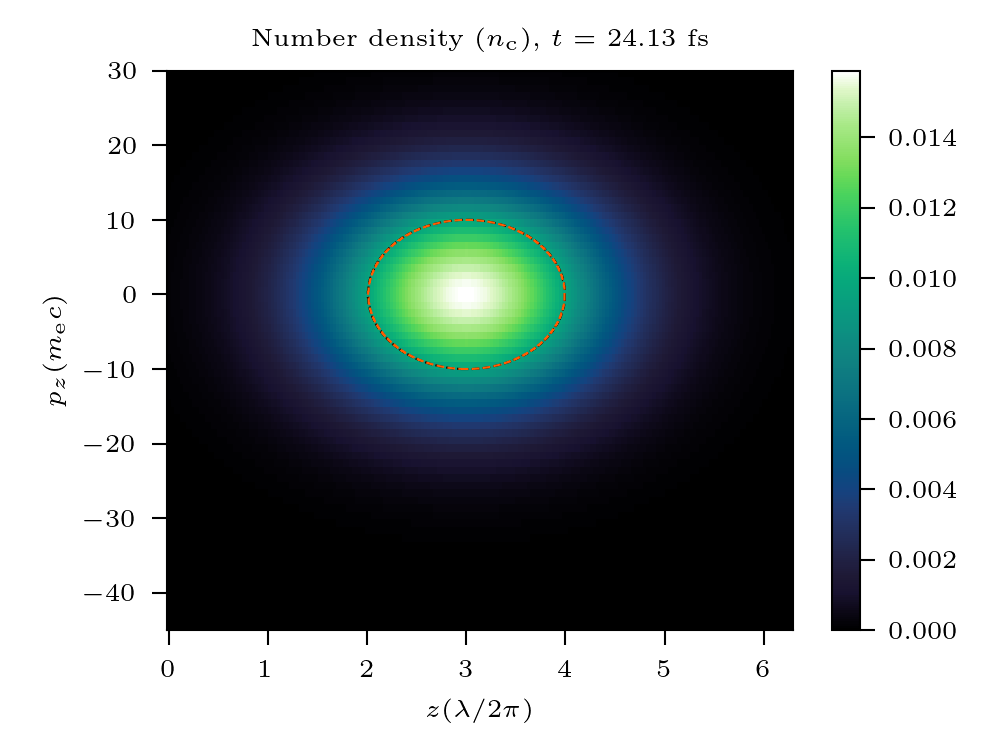
\includegraphics[width=0.7\linewidth]{figures/appendix/emittance_normal}
	\caption[Emittance calculation for an ideal Gaussian distribution in phase space.]{Emittance calculation for an ideal Gaussian distribution in phase space, $f_\mathrm{n}(z,p_z) = 1/(2\pi s_zs_{pz})\exp[-((z-m_z)^2/(2s_z^2) + (p_z-m_{pz})^2/(2s_{pz}^2))]$, centred at ($m_z$,$m_{pz}$) = (3,0) with standard deviations ($s_z$,$s_{pz}$) = (1,10).}
	\label{fig:emittancenormal}
\end{figure}
The contour is numerically calculated to contain \qty{39.4 \pm .1}{\%} of the particles, compared to 39.3 \% from theory. Here the discrepancy arises from the finite grid on which the distribution is defined.

\section{The Bourdier method}\label{sec:app-bourdier}
The Bourdier method enables the modelling of an obliquely incident laser pulse in 1D geometry \cite{bourdierObliqueIncidenceStrong1983}. While some of this section may seem trivial, it is frequently misquoted in the literature. It therefore seems of great importance to provide a full derivation.

Consider a photon incident on a plasma block at angle $\theta$ as in Figure \ref{fig:miscreferenceframesboosted1d}.
\begin{figure}
	\centering
	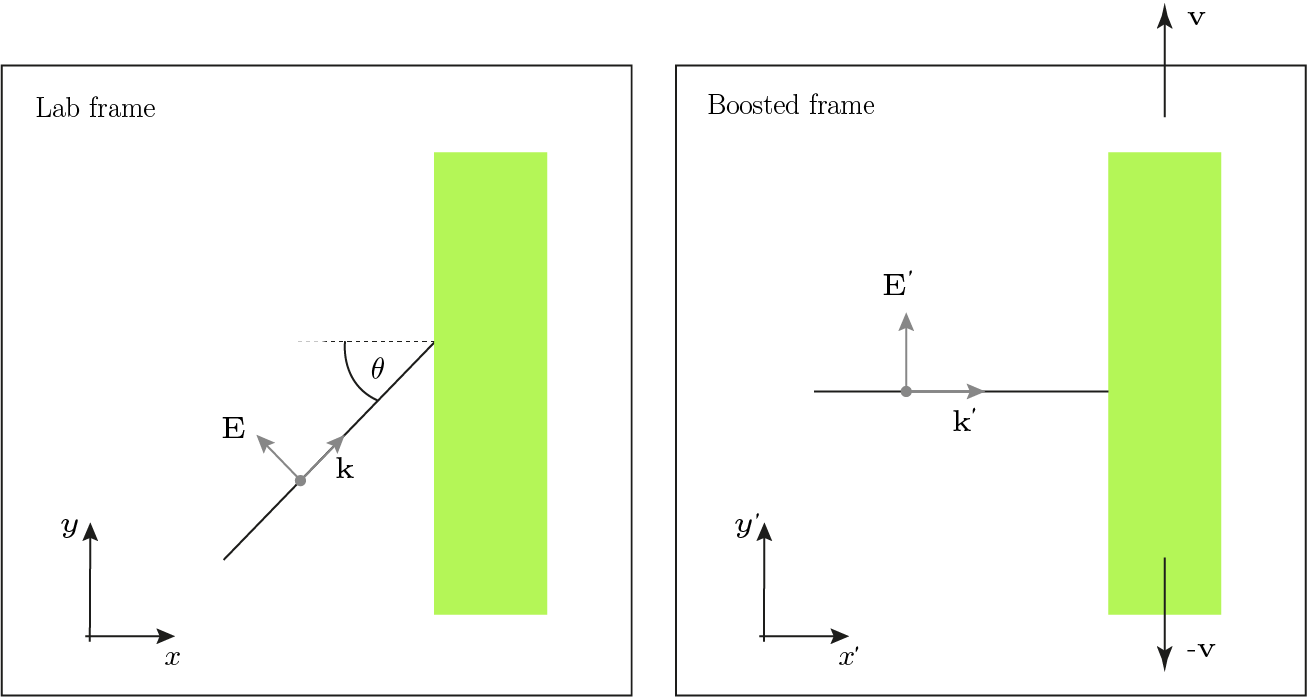
\includegraphics[width=1\linewidth]{figures/misc/misc_reference_frames_boosted_1D}
	\caption{}
	\label{fig:miscreferenceframesboosted1d}
\end{figure}
A boost is applied with velocity $\mathbf{v}$ to the laboratory frame such that the photon is normally incident on the now streaming plasma at velocity $-\mathbf{v}$. The velocity transformation for the photon's velocity, $\mathbf{u}$, parallel to the boost is
\begin{equation}
	\mathbf{u}'_\parallel = \frac{\mathbf{u}_\parallel - \mathbf{v}}{1-\mathbf{u}\cdot\mathbf{v}/c^2}.
\end{equation}
Setting  $\mathbf{u}'_\parallel = 0$, it is clear that
\begin{equation}
	\mathbf{v} = \mathbf{u}_\parallel = c\sin\theta \hat{\mathbf{y}}
\end{equation}
in this geometry and 
\begin{equation}
	\gamma_\mathbf{v} = \frac{1}{\sqrt{1-\mathbf{v}^2/c^2}}=\sec\theta.
\end{equation}
Since Snell's law is frame invariant, the photon remains normal as it propagates into the skin depth of the plasma, a frame in which the interaction reduces to a 1D problem has been successfully found for all $\theta < \pi/2$. Those familiar with the topic may wonder how this is possible considering the `ripples' that can be observed on the plasma surface for oblique incidence. The explanation for this is of course the relativity of simultaneity. 

It remains to determine how do all the relevant quantities transform as such a boost is applied. Starting with an simple one: the photon's wave four-vector is 
\begin{equation}
	\mathbf{K}^\mathrm{\mu} = \left(\frac{\omega}{c},\mathbf{k}\right)
\end{equation}
and thus the frequency transforms as
\begin{equation}
	\frac{\omega}{c} = \gamma_\mathbf{v}\left(\frac{\omega'}{c}-\frac{\mathbf{v}}{c}\cdot\mathbf{k'}\right).
\end{equation}
Since $\mathbf{v}\cdot\mathbf{k'} = 0$, 
\begin{equation}\label{eq:boost_omega}
	\omega' = \omega\cos\theta .
\end{equation}
As 
\begin{equation}
	n'_\mathrm{c} = \frac{m_\mathrm{e}(\omega')^2}{4\pi e^2},
\end{equation}
\begin{equation}\label{eq:boost_nc}
	n'_\mathrm{c} =n_\mathrm{c} \cos^2\theta ,
\end{equation}
while the plasma block will be Lorentz contracted along $\hat{\mathbf{y}}$. Hence, the number density of electrons will increase as
\begin{equation}
	n'_\mathrm{e} = \frac{n'_\mathrm{e}}{\cos\theta}
\end{equation}
leading to the perhaps unexpected
\begin{equation}
	\bar{n}'_\mathrm{e} = \frac{\bar{n}_\mathrm{e}}{\cos^3\theta}.
\end{equation}
Time is dilated 
\begin{equation}
	t' = \frac{t}{\cos\theta}.
\end{equation}

Consider now the more general case where the photon's electric field is rotated out of the $x$-$y$ plane, \textit{i.e.}
\begin{equation}
	\mathbf{E} = E_0(-\cos\phi\sin\theta,\cos\phi\cos\theta,\sin\phi)
\end{equation}
and correspondingly
\begin{equation}
	\mathbf{B} = \frac{\hat{\mathbf{k}} \times \mathbf{E}}{c}= \frac{E_0}{c}(\sin\phi\sin\theta,-\sin\phi\cos\theta,\cos\phi).
\end{equation}
The Lorentz transformations for electro-magnetic fields are
\begin{equation}
	\mathbf{E}'_\parallel = \mathbf{E}_\parallel,
\end{equation}
\begin{equation}
	\mathbf{B}'_\parallel = \mathbf{B}_\parallel,
\end{equation}
\begin{equation}
	\mathbf{E}'_\perp = \gamma_\mathbf{v}(\mathbf{E}_\perp + \mathbf{v} \times \mathbf{B}),
\end{equation}
\begin{equation}
	\mathbf{B}'_\perp = \gamma_\mathbf{v}(\mathbf{B}_\perp - \mathbf{v} \times \mathbf{E}/c^2).
\end{equation}
Using the above expressions for $\mathbf{E}_\perp$ and $\mathbf{E}_\parallel$ and transforming to the boosted frame,
\begin{equation}
	\mathbf{E}' = E_0\cos\theta (0,\cos\phi,\sin\phi).
\end{equation}
As anticipated for normal incidence there is no component of the E-field normal to the surface. Conveniently, the polarisation of the incident photon is unchanged despite having components both parallel and perpendicular to the transformation and 
\begin{equation}
	|\mathbf{E}'| = |\mathbf{E}|\cos\theta.
\end{equation}
The picture can now be completed. Since
\begin{equation}
	a_0' = \frac{e|\mathbf{E}'|}{m_\mathrm{e}e\omega'}
\end{equation}
it follows that \cite{bourdierDynamicsChargedParticle2001}
\begin{equation}
	a_0' = a_0,
\end{equation}
\begin{equation}
	S' = \frac{S}{\cos^3\theta}.
\end{equation}

Normalised Smilei units now come into their own in this new framework. In Smilei units, distances, times and vector potentials are unchanged by the interaction and can simply be extracted from the simulation in the required frame by multiplying by the frame of interest's reference quantity. Care must still be taken with densities.





%%%%% REFERENCES

% JEM: Quote for the top of references (just like a chapter quote if you're using them).  Comment to skip.
\begin{savequote}[8cm]
The first kind of intellectual and artistic personality belongs to the hedgehogs, the second to the foxes \dots
  \qauthor{--- Sir Isaiah Berlin \cite{berlin_hedgehog_2013}}
\end{savequote}

\setlength{\baselineskip}{0pt} % JEM: Single-space References

{\renewcommand*\MakeUppercase[1]{#1}%
\printbibliography[heading=bibintoc,title={\bibtitle}]}


\end{document}
